\documentclass
[
	12pt, %Schriftgröße
	a4paper, %Papierformat
	twoside, %einseitiger Druck, für zweiseitigen Druck weglassen
	openany, %neue Kapitel dürfen auch auf linker Seite beginnen (beidseitiger Druck), sonst openright (default)
	chapterprefix, %Kapitelüberschriften zu Beginn eines Kapitels anzeigen
	listof=totoc, %Verzeichnisse (Abbildungen/Tabellen) im Inhaltsverzeichnis aufführen
	%draft, %Entwurfsmodus: lässt Links und Abbildungen weg, zeigt übervolle Zeilen an, wird schneller gesetzt
]{scrbook}

\newcommand*{\universitaet}[1]{\def\universitaet{#1}}
\newcommand*{\fach}[1]{\def\fach{#1}}
\newcommand*{\arbeitsart}[1]{\def\arbeitsart{#1}}
\newcommand*{\titel}[1]{\def\titel{#1}}
\newcommand*{\autor}[1]{\def\autor{#1}}
\newcommand*{\gutachterEins}[1]{\def\gutachterEins{#1}}
\newcommand*{\gutachterZwei}[1]{\def\gutachterZwei{#1}}
\newcommand*{\gutachterDrei}[1]{\def\gutachterDrei{#1}}
\newcommand*{\abteilung}[1]{\def\abteilung{#1}}
\newcommand*{\department}[1]{\def\department{#1}}
\newcommand*{\ort}[1]{\def\ort{#1}}
\newcommand*{\datum}[1]{\def\datum{#1}}

%---------------------------------
%---Sprache, Schrift & Encoding---
%---------------------------------
\setlength {\marginparwidth }{2cm}
\usepackage[colorinlistoftodos]{todonotes}

\usepackage[ngerman]{babel} %neue deutsche Rechtschreibung
\usepackage[utf8]{inputenc} %alternativ: ansinew (windows), latin1, latin9 (Linux/UNIX/Mac)

%\usepackage[T1]{fontenc} %einkommentieren, wenn Buchstaben/Schriftbild schief aussehen!
%\usepackage{lmodern} %andere Schrift, sieht evtl. besser aus

%------------
%---Layout---
%------------

\usepackage
[
	left=3cm, %linker Seitenrand
	right=3cm, %rechter Seitenrand
	top=2.5cm, %oberer Seitenrand
	bottom=2.5cm, %unterer Seitenrand
]{geometry}
\usepackage[onehalfspacing]{setspace} %1,5-facher Zeilenabstand

%\usepackage{indentfirst} %rückt auch den ersten Absatz eines (Unter)abschnitts ein, so wie alle anderen Absätze auch

\usepackage
[
	headsepline, %Kopfzeile durch Querlinie abheben
%	footsepline, %Fußzeile durch Querlinie abheben
	draft=false, %Kopf-/Fußzeile auch im draft-Modus (siehe documentclass) anzeigen
]{scrlayer-scrpage}

\clearpairofpagestyles
\ihead[]{\headmark} %Kapitel-/Abschnittsname innen in der Kopfzeile, außer zu Beginn neuer Kapitel
%\chead[]{}
\ohead*[]{\pagemark} %Seitenzahl außen in der Kopfzeile, außer zu Beginn neuer Kapitel
%\ifoot[]{}
%\cfoot[]{}
\ofoot*[\pagemark]{} %Seitenzahl außen in die Fußzeile, aber nur zu Beginn neuer Kapitel

\renewcommand*\chapterformat{\chapapp~\thechapter} %Kapitelüberschriften in der Form Kapitel~<Nummer>
\newcommand{\source}[1]{\caption*{\hfill Quelle: {#1}} }

\DeclareTOCStyleEntry[numwidth=3em]{tocline}{figure} % Für Abbildungsverzeichnis
\DeclareTOCStyleEntry[numwidth=3em]{tocline}{table} % Für Tabellenverzeichnis

%-----------
%---Mathe---
%-----------

\usepackage{amsmath}
\usepackage{amsfonts}
\usepackage{amssymb}

%---------------
%---Sonstiges---
%---------------

\usepackage[square,sort,comma,numbers]{natbib} %ermöglicht die Verwendung von \citet{} und \citep{}
\bibliographystyle{alphaurl} %Geändert, vorher: dinat | Zitierstil: andere auch möglich, z.B. alphadin, plain, ...

\usepackage{caption}
\usepackage{subcaption}
\usepackage{graphicx}

\usepackage[german]{authblk}

\usepackage{enumerate}
\usepackage{paralist}

\usepackage{longtable}
\usepackage{multirow}
\usepackage{makecell}
\usepackage{blindtext}
\usepackage{ltablex}
\usepackage{float}
\usepackage{listings}
\usepackage{adjustbox}
\usepackage{booktabs}
\usepackage[utf8]{inputenc}
% \lstset{basicstyle=\ttfamily\footnotesize,breaklines=true}
\renewcommand{\lstlistlistingname}{Quellcodeverzeichnis}

\lstset{
language=java,
basicstyle=\small\sffamily,
numbers=left,
numberstyle=\tiny,
frame=tb,
columns=fullflexible,
showstringspaces=false
}

%------------------
%---Links & URLs---
%------------------

%hyperref möglichst als letztes package laden (es gibt aber Ausnahmen)!
\usepackage[hyphens]{url}
%\usepackage[draft]{hyperref} %falls Fehler beim Compilieren auftreten aufgrund von hyperlinks. Hinweis: Ist der draft Modus eingeschaltet, funktionieren KEINE Referanzen mehr.
\usepackage{hyperref} %für Referenzen, Verweise, Links, ...
\hypersetup{
     urlcolor=black,
}

\usepackage[nohyperlinks]{acronym} %Für Abkürzungen

\newcommand*\signature[2][6cm]{\vspace*{2cm}\parbox{#1}{\hrulefill\par#2}}


%-----------------------------
%---Variablen zum ausfüllen---
%-----------------------------

\universitaet{Carl von Ossietzky Universität Oldenburg}
\fach{Informatik} %Informatik, ...
\arbeitsart{Masterarbeit} 
\titel{Entwicklung von prädiktiven und reaktiven Lösungsansätzen für das MRCPSP auf Basis von Metaheuristiken}
\autor{René Kuchenbuch, B. Sc.}
\gutachterEins{apl. Prof. Dr.-Ing. Jürgen Sauer}
\gutachterZwei{Julius Möller, M. Sc.}
\abteilung{Abteilung Systemanalyse und -optimierung}
\department{Department für Informatik}
\ort{Oldenburg}
\datum{\today} 

%----------------
%---Titelseite---
%----------------

\setcounter{secnumdepth}{4}
\setcounter{tocdepth}{4}

\begin{document}

\frontmatter %römische Seitennummerierung für den Anfang

\makeatletter
\begin{titlepage}
\centering
\begin{figure}[htb]
  \centering
  \begin{subfigure}{0.5\textwidth}
    \centering
    
\includegraphics[scale=1.8]{assets/img/uni_ol_logo.png}
    \end{subfigure}%
    \begin{subfigure}{0.5\textwidth}
      \centering
      
\includegraphics[scale=0.35]{assets/img/abteilungslogo.jpg}
    \end{subfigure}
\end{figure}

{\scshape\Large\universitaet\par}
\vspace{1cm}
{\scshape\normalsize\fach\par}
{\scshape\normalsize\arbeitsart\par}

\vfill

\hrule
\vspace{1cm}
{\LARGE\bfseries\titel\par}
\vspace{1cm}
\hrule

\vfill

\begin{minipage}[t]{0.5\textwidth}
  \begin{flushleft}
    {\normalsize\itshape vorgelegt von:\par}
    {\normalsize Autor: \autor\par}
    {\normalsize Studiengang: Informatik (M. Sc.) \par}
    {\normalsize Matr. Nr.: 5896997}
  \end{flushleft}
\end{minipage}
\begin{minipage}[t]{0.4\textwidth}
  \begin{flushright}
    {\normalsize\itshape Betreuender Gutachter:\par}
    {\normalsize\gutachterEins}
    \hbox to 3cm{}%

    {\normalsize\itshape Zweiter Gutachter:\par}
    {\normalsize\gutachterZwei}
  \end{flushright}
\end{minipage}

\vfill

{\normalsize\abteilung\par}
{\normalsize\department\par}
\vspace{1cm}
{\normalsize\ort{}, \datum\par}
\end{titlepage}
\makeatother

%---------------
%---Disclaimer---
%---------------

\input{pages/X1_Sonstiges/X3_Disclaimer}

%---------------
%---Abstracts---
%---------------

\chapter*{Abstract (deutsch)}
\thispagestyle{empty}
Das \acf{mrcpsp} stellt ein NP-vollständiges Optimierungsproblem dar, welches sich mit der Erzeugung von Projektplänen mit Ressourcenbeschränkungen befasst. Unsicherheiten, wie z. B. Verspätungen führen dazu, dass ein Projektplan nicht mehr in geplanter Zeit vollendet werden kann. \\

Das Ziel der Masterarbeit befasst sich zunächst mit der Suche von Basiszeitplänen für Projekte mit Hilfe von Metaheuristiken, welche die Projektdauer minimieren sollen. Anschließend gilt es prädiktive und reaktive Verfahren zu selektieren um die einhergehenden Verspätungen durch Unsicherheiten zu minimieren. \glqq Welche Auswirkungen haben prädiktive und reaktive Ansätze für das MRCPSP auf Basis von metaheuristischen Algorithmen bei der Erstellung von Zeitplänen in Bezug auf die Projektdauer bei Verspätungen?\grqq{} stellt die Forschungsfrage der Thesis. \\

Diese Forschungsfrage wurde über eine quantitative Studie mit Hilfe eines zu implementierenden Framework beantwortet. Hierfür werden unterschiedliche Metaheuristiken konzipiert und implementiert. Als prädiktives Verfahren wurde die Robustheitsoptimierung und als reaktives Verfahren die Reparatur eines Zeitplans über eine Kostenfunktion zum Unsicherheitszeitpunkt ausgewählt. Über das Durchlaufen der pro-, prä- und reaktiven Verfahren auf eine gemeinsame Benchmark-Basis und auf eine Vielzahl an zufällig generierten Unsicherheitsszenarien konnten Daten für die quantitative Analyse erhoben werden. \\

Die Daten für \acf{mrcpsp} zeigten, dass beide Verfahren Verspätungen durch Aktivitätsstörungen signifikant minimieren, wobei das prädiktive Verfahren insbesondere für kleinere und das reaktive Verfahren für komplexere Unsicherheitsszenarien geeignet ist. 

\chapter*{Abstract (english)}
\thispagestyle{empty}
The \acf{mrcpsp} represents an NP-complete optimization problem dealing with the generation of project plans with resource constraints. Uncertainties, such as delays, cause a project plan to fail to complete in planned time. \\

The goal of the master thesis is first to find baseline schedules for projects using metaheuristics, which should minimize the project duration. Subsequently, predictive and reactive methods have to be selected in order to minimize the associated delays due to uncertainties. \glqq What is the impact of predictive and reactive approaches for MRCPSP based on metaheuristic algorithms in generating schedules in terms of project duration in the presence of delays?\grqq{} poses the research question of the thesis. \\

This research question was answered via a quantitative study using a framework that needed to be implemented. For this purpose, different metaheuristics are designed and implemented. Robustness optimization was selected as the predictive procedure and repair of a schedule via a cost function at the uncertainty time as the reactive procedure. By running the proactive, preactive and reactive procedures on a common benchmark basis and on a variety of randomly generated uncertainty scenarios, data for quantitative analysis could be obtained. \\

The data of the \acs{mrcpsp} showed that both methods significantly minimize delays due to activity perturbations, with the predictive method being particularly suitable for smaller uncertainty scenarios and the reactive method for more complex scenarios. 

%-------------------
%---Verzeichnisse---
%-------------------

\setcounter{page}{0}
\tableofcontents

\listoffigures
\listoftables
\lstlistoflistings
 
\chapter{Abkürzungsverzeichnis}

\begin{acronym}
\acro{rcpsp}[RCPSP]{Resource-Constrained Project Scheduling Problem}
\acro{mrcpsp}[MRCPSP]{Multi-Mode Resource-Constrained Project Scheduling Problem}
\acro{jsp}[JSP]{Job-Shop Problem}
\acro{sgs}[SGS]{Schedule Generation Scheme}
\acro{ssgs}[S-SGS]{Serial Schedule Generation Scheme}
\acro{psgs}[P-SGS]{Parallel Schedule Generation Scheme}
\acro{EST}[EST]{Earliest Starting Time}
\acro{EFT}[EFT]{Earliest Finishing Time}
\acro{LST}[LST]{Latest Starting Time}
\acro{LFT}[LFT]{Latest Finishing Time}
\acro{RS}[RS]{Random Sampling}
\acro{BRS}[BRS]{Biased Random Sampling}
\acro{RBRS}[RBRS]{Regret Based Biased Random Sampling}
\acro{LS}[LS]{Local Search}
\acro{TS}[TS]{Tabu Search}
\acro{SA}[SA]{Simulated Annealing}
\acro{GA}[GA]{Genetic Algorithm}
\acro{POJO}[POJO]{Plain Old Java Object}

\end{acronym} 

%---------------
%---Hauptteil---
%---------------

\mainmatter

\chapter{Einleitung} \label{ch:Einleitung}

Dieses Kapitel der Einführung beginnt zunächst mit dem Abschnitt \ref{sec:Motivation}, welcher das Thema der Masterarbeit motiviert. Im Folgeabschnitt werden die anzustrebenden Ziele der Masterarbeit einschließlich der Forschungsfrage und die dazugehörigen Unterfragen vorgestellt. Der Aufbau der vorliegenden Arbeit wird anschließend im Abschnitt \ref{sec:Aufbau} erläutert.

\section{Motivation} \label{sec:Motivation}

\glqq Plans are worthless, but planning is everything!\grqq{} \cite[S. 235]{eisenhower_dwight_1958} Dwight D. Eisenhower vom 14. November 1957. In dem Zitat vom 34. Präsidenten der USA steckt viel Bedeutung, denn diese Aussage kann dahingehend interpretiert werden, dass in Plänen Ereignisse und Eventualitäten nicht stets berücksichtigt werden. Zu den häufigen Fehlern innerhalb des Projektmanagements gehören Fehlentscheidungen, unklare Abhängigkeiten, Ressourcenknappheiten und vieles weitere \cite[vgl.][S. 74]{nelson_it_2007}. Die Folgen von solchen Fehlern sind nicht zuletzt Verspätungen innerhalb des Zeitplans.  \\

Die ressourcenbeschränkte Projektplanung ist ein Feld aus dem Bereich Operation Management und befasst sich mit der Planung von Projekten mit Ressourcen. Ein Projekt besteht aus einzelnen Aktivitäten, welche wiederum Ressourcen zur Vollendung benötigen. Ein Projekt kann beispielsweise die Entwicklung eines neuen Produktes sein, das Bauen eines Gebäudes, aber auch schon das Backen eines Kuchens. Projekte mit Ressourcenbeschränkungen sind bereits zudem in vielen Unternehmen allgegenwärtig. \cite[vgl.][S. 1 f.]{kellenbrink_ressourcenbeschrankte_2014} \\

Zeitpläne ohne Ressourcenbeschränkungen können über Vor- und Rückwärtskal-kulationen erstellt werden \cite[vgl.][S. 9 f.]{kellenbrink_ressourcenbeschrankte_2014}. Jedoch stellen die Beschränkungen bei der ressourcenbeschränkten Projektplanung ein Problem dar, da die Ressourcen innerhalb der Aktivitätsausführung durchgehend zur Verfügung stehen müssen, womit andere Verfahren, wie (Meta-)Heuristiken benötigt werden, um gültige Zeitpläne zu erstellen \cite[vgl.][S. 11]{kellenbrink_ressourcenbeschrankte_2014}. Dies stellt das ressourcenbeschränkte Projektplanungsproblem (RCPSP) dar \cite[vgl.][S. 11]{kellenbrink_ressourcenbeschrankte_2014}, welches als ein NP-hartes Optimierungsproblem angesehen wird \cite[vgl.][S. 2]{kolisch_heuristic_1998}. Im Mittelpunkt der Masterarbeit steht eine Problemerweiterung des RCPSP, nämlich das Multimodus ressourcenbeschränkte Projektplanungsproblem (MRCPSP) welches Aktivitäten über eine von mehreren zur Verfügung stehenden Alternativen durchlaufen werden muss \cite[vgl.][S. 596]{wuliang_improved_2014}. \\

Der Umgang mit Unsicherheiten, sei es aufgrund einer Fehlplanung, tatsächlicher Ressourcenknappheiten, Krankheiten innerhalb des Personals oder weiteren Gründen stellt ebenfalls einen wesentlicher Faktor der Masterarbeit dar. Hierfür existieren verschiedene Verfahren, wie die proaktive, prädiktive oder reaktive Planung. Bei der proaktiven Planung werden Unsicherheiten ignoriert. Der prädiktive Ansatz nutzt weitere Kennziffern, wie die Robustheit eines Zeitplans, welche es zu maximieren gilt, um so Verspätungen durch Unsicherheiten zu verringern. Beim reaktiven Ansatz wird zum Zeitpunkt einer Unsicherheit reagiert, um so den Zeitplan zu reparieren oder einen neuen Zeitplan zu erstellen. \cite[vgl.][S. 404 f.]{brcic_resource_2012} \\

Zum Zeitpunkt der Masterarbeit bietet das Multi-Mode Ressource Constrained Project Scheduling Problem (MRCPSP) mit dem Umgang von Unsicherheiten weiterhin ein hohes Forschungspotential. Ein direkter Vergleich von Verfahren für den Umgang mit Unsicherheiten wurde für das MRCPSP noch nicht gezogen. Die Kombination von Metaheuristiken mit den pro-, prä-, reaktiven Methoden gilt es zudem ebenfalls zu evaluieren. 
\section{Problemstellung} \label{sec:Ziele}

Das Problem der Unsicherheiten gilt es für das \ac{mrcpsp} zu lösen, um so die einhergehenden Verspätungen so gering wie möglich zu halten. Im Rahmen der Masterarbeit wird daher die folgende Forschungsfrage aufgestellt: Welche Auswirkungen haben prädiktive und reaktive Ansätze für das MRCPSP auf Basis von metaheuristischen Algorithmen bei der Erstellung von Zeitplänen in Bezug auf die Projektdauer bei Verspätungen? \\

Die Forschungsfrage wird mithilfe weiterer Unterfragen gestützt. Welche prädiktiven und reaktiven Ansätze können für das MRCPSP in Kombination mit metaheuristischen Algorithmen angewandt werden? Lässt sich ein Vergleich zwischen prädiktiven und reaktiven Ansätzen auf das Ergebnis in Bezug zur Projektdauer ziehen? Welchen Einfluss haben hierbei Metaheuristiken zur Findung von \glqq guten\grqq{} Lösungen? \\

Um die Unterfragen beantworten zu können müssen die proaktiven, prädiktiven und reaktiven Verfahren auf Benchmarks mit Unsicherheitsszenarien angewandt werden. Diese Benchmarks müssen zunächst für das MRCPSP selektiert werden. Zudem gilt es die Unsicherheitsszenarien innerhalb der Benchmarks zu konzipieren und zu integrieren. Um geeignete Lösungen für das Problem zu finden sollen Metaheuristiken eingesetzt werden. Die Auswahl und die Integrierung, aber auch deren Evaluierung der Metaheuristiken über einen Vergleich der gefundenen Projektdauern sind ebenfalls wesentlicher Bestandteil dieser Arbeit. 
\section{Aufbau der Arbeit} \label{sec:Aufbau}

Zu Beginn der Arbeit wurde bereits das Thema der Masterarbeit motiviert und die Ziele innerhalb der Problemstellung definiert. Die folgenden Kapitel der Arbeit befassen sich mit den folgenden Inhalten:
\begin{description}
    \item[Kapitel 2] In dem Kapitel gilt es die theoretischen Grundlagen des (Multi-Mode) \acl{rcpsp} zu erläutern. Sowohl das Grundproblem als auch die Multi-Mode Problemerweiterung werden zunächst formal definiert. Zudem sollen heuristische Lösungsansätze für das \acs{mrcpsp} vorgestellt werden. Des Weiteren werden in dem Kapitel die theoretischen Grundlagen von einer Auswahl an Metaheuristiken vorgestellt. Zuletzt wird in dem Kapitel der aktuelle Stand der Forschung präsentiert, in welcher das Thema der Masterarbeit eingeordnet wird. \\ 
    \item[Kapitel 3] Das darauffolgende Kapitel befasst sich mit der Konzeption des MRCPSP-Framework. Hierbei wird im ersten Abschnitt gemäß der Problemstellung basierend auf dem Stand der Forschung ein Konzeptüberblick gegeben. Relevante Teilkomponenten des Konzepts werden im weiteren Verlauf des Kapitels behandelt. \\
    \item[Kapitel 4] Dieses Kapitel basiert auf dem im vorherigen Kapitel vorgestellten Konzept und geht auf die konkrete Umsetzung des MRCPSP-Framework ein. Einleitend wird zunächst die Struktur des Frameworks vorgestellt. Im Anschluss werden einzelne Teilkomponenten erläutert, welche für die Beantwortung der Forschungsfragen relevant sind. \\
    \item[Kapitel 5] Wesentlicher Bestandteil des Kapitels ist der quantitative Vergleich der entwickelten pre-, prä- und reaktiven Verfahren und Metaheuristiken gemäß der Problemstellung. \\ 
    \item[Kapitel 6] Das abschließende Kapitel \ref{ch:Zusammenfassung}, bestehend aus dem Fazit und dem Ausblick, beantwortet die Forschungsfrage und dessen Unterfragen anhand der Evaluation und fasst die Ergebnisse der Arbeit zusammen. Themen und Problemstellungen für weiterführende Arbeiten sind dem Ausblick zu entnehmen. \\ 
\end{description}

\chapter{Grundlagen} \label{ch:Grundlagen}

Dieses Kapitel dient zur Einführung der Schlüsselthemen der Masterthesis. Wesentliches Thema der Arbeit stellt das Optimierungsproblem (Multi-Mode) Resource-Constrained Project Scheduling Problem. Dieses (M)\ac{rcpsp} wird zunächst im Abschnitt \ref{sec:MRCPSP} erläutert. Metaheuristiken stellen eine generische Möglichkeit zur Lösung von Optimierungsproblemen dar. Abschnitt \ref{sec:Metaheuristiken} zeigt die Funktionsweise von verschiedenen Metaheuristiken auf. 

\section{(Multi-Mode) Resource-Constrained Project Scheduling Problem} \label{sec:MRCPSP}

Eines der am meisten verbreiteten Optimierungsprobleme stellt das Resource Constrained Project Scheduling Problem dar. Dieses Problem findet insbesondere bei der Projektplanung, aber auch in vielen Bereichen der Gegenwart einen realistischen Bezug. Das Problem bezieht sich auf das Finden von optimalen Schedules (dt. Zeitplänen) von festgelegten Projektablaufplänen, wobei die Aktivitäten erneuerbare Ressourcenanforderungen (z B. Maschinen oder menschliche Arbeitskraft) aufweisen. Optimale Schedules können nicht ohne Weiteres bestimmt werden, folglich müssen für einen gegebenen Projektplan alle Möglichkeiten durchiteriert werden. Dies stellt durch die Komplexität des Lösungsraums ein $\mathcal{NP}$-hartes Problem dar \cite[vgl.][S. 2]{kolisch_heuristic_1998}. Das \ac{rcpsp}-Basisproblem wird im Abschnitt \ref{subsec:MRCPSP_RCPSP} erläutert. \\

Das RCPSP sieht bei Aktivitäten nur eine Art der Ausführung vor. Zudem berück-sichtigt das Grundproblem keine nicht-erneuerbaren Ressourcen, wie z. B. Geldmengen oder Verbrauchsgüter, welche insbesondere in der Praxis und in Projekten wesentliche Bestandteile sind. Diese Aspekte werden in einer Problemerweiterung, nämlich dem Multi-Mode Resource-Constrained Project Scheduling Problem berücksichtigt \cite[vgl.][S. 596 f.]{wuliang_improved_2014}, welche im Abschnitt \ref{subsec:MRCPSP_MM} beleuchtet werden. \\

Um zunächst mögliche, wenn auch nicht optimale Lösungen zu erzeugen, wird unter anderem das Verfahren \ac{ssgs} eingesetzt. Dieses ermöglicht das Aufbauen von Schedules über das inkrementelle Erweitern von partiellen Schedules \cite[vgl.][S. 3]{kolisch_heuristic_1998}. \ac{ssgs} findet bei Heuristiken, aber auch in Metaheuristiken Verwendung \cite[vgl.][S. 3]{kolisch_heuristic_1998}. Beleuchtet wird das Konzept einschließlich der gängigen Heuristiken im Abschnitt \ref{subsec:SGS}. \\

In der Realität sind Unsicherheiten in Zeitplänen nicht abwegig. Diese können beispielsweise in Form von Verspätungen, aber auch über erhöhten Ressourcenverbrauch auftreten. Diese Thematik samt Möglichkeiten zum Umgang des Problems werden im Abschnitt \ref{subsec:MRCPSP_Unsicherheiten} erläutert. 


\subsection{Resource-Constrained Project Scheduling Problem} \label{subsec:MRCPSP_RCPSP}

% Einfach

Eines der am meisten behandelten Optimierungsprobleme stellt das \ac{rcpsp} dar. Das grundlegende \ac{rcpsp} behandelt das Finden von Schedules (dt. Zeitplänen) bei einem gegebenen Projektplan. Ein Projekt besteht aus einer Menge von Aktivitäten $J = \{ 0, ..., j, j + 1 \}$, wobei es sich $J_0$ und $J_{j+1}$ um Dummy-Aktivitäten handeln, welche den Projektstart bzw. das Projektende repräsentieren. Aktivitäten können untereinander in Beziehung stehen, sodass eine Aktivität $j \in J$ erst gestartet werden kann, wenn alle seine Vorgänger $P(j) \in 2^J$ fertiggestellt wurden. Diese besitzen im Grundproblem zudem eine feste Dauer $d_j \in \mathbb{N}_0$ und Ressourcenanforderungen $r_{j,k} \in \mathbb{N}_0$. Bei den Ressourcen wird zwischen erneuerbaren Ressourcenarten $K = \{1, ..., R\}$ unterschieden. Alle Ressourcenarten stehen innerhalb eines Projektes nur in limitierter Anzahl $R_{k} \in \mathbb{N}$ zur Verfügung, welche während der Projektausführung über die Aktivitäten aufgeteilt werden müssen. Für die Projektstart- und Ende-Aktivitäten gelten zudem $\forall \, k \in K: r_{j,k} = 0$ und $d_j = 0$. Diese Restriktion zeigt auf, dass keine Ressourcen- und Zeitanforderungen für die Aktivitäten gegeben sind. Zudem dürfen Aktivitäten nicht bei der Ausführung unterbrochen werden. \cite[vgl.][S. 1 ff.]{kolisch_heuristic_1998}. \\

Das Ziel des \ac{rcpsp} liegt darin, den Zeitplan mit der minimalsten Makespan (zu dt. Projektausführungsdauer) zu bestimmen. Formal wird die Zielfunktion des \ac{rcpsp} von \cite[S. 1]{kolisch_heuristic_1998} vergleichsweise wie folgt beschrieben:
\begin{align}
    \min \, F_{n+1} = \min \, C_{max} & \qquad \textit{es muss gelten:} \label{align:rcpsp_goal} \\
    \forall j \in J, h \in P_j:\, & F_h \leq F_j - d_j \label{align:rcpsp_constraint1} \\
    \forall k \in K, t \geq 0:\, & \sum_{j \in A(t)} r_{j,k} \leq R_k  \label{align:rcpsp_constraint2}
\end{align}
Die Menge der zum Zeitpunkt $t$ ausgeführten Aktivitäten wird über $A(t)$ angegeben. $F_j$ entspricht der Endzeit einer Aktivität $j \in J$. Eine Aktivität kann erst gestartet werden, wenn alle unmittelbaren Vorgänger abgeschlossen wurden (vgl. Formel \ref{align:rcpsp_constraint1}). Formel \ref{align:rcpsp_constraint2} gewährleistet, dass die Kapazitäten von den erneuerbaren Ressourcen zu jedem Zeitpunkt nicht überschritten werden dürfen. 

\begin{figure}[H]
    \centering
    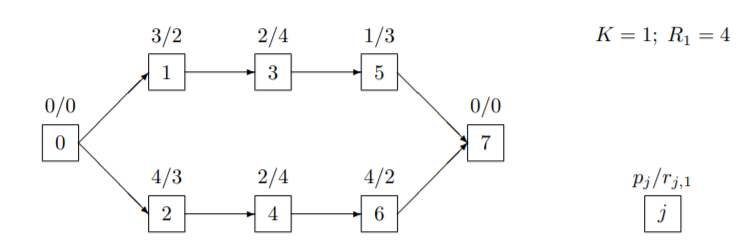
\includegraphics[width=1\textwidth]{assets/img/02_Grundlagen/ExampleProjectRCPSP_Plan.png}
    \caption{Graphen-Darstellung eines \ac{rcpsp} Beispiel-Projektplans mit $|J| = 8$ Aktivitäten} 
    \label{img:example_rcpsp}
    \source{\cite[][S. 2]{kolisch_heuristic_1998}}
\end{figure}

Abbildung \ref{img:example_rcpsp} stellt einen beispielhaften Projektplan mit $|J| = 8$ Aktivitäten als Knoten samt deren Ressourcen- und Zeitanforderungen dar. Diese stehen oberhalb der Knoten in der Schreibweise $d_j / r_{r,i}$. $J_0$ und $J_7$ entsprechen den Dummyknoten, welche keine Ressourcen- und Zeitanforderungen aufweisen. Die Kanten zeigen Beziehungen zu den Nachfolgeaktivitäten auf. Zudem steht eine erneuerbare Ressourcenart mit einer Kapazität von 4 Mengeneinheiten ($R_1 = 4$) zur Verfügung. 

\begin{figure}[H]
    \centering
    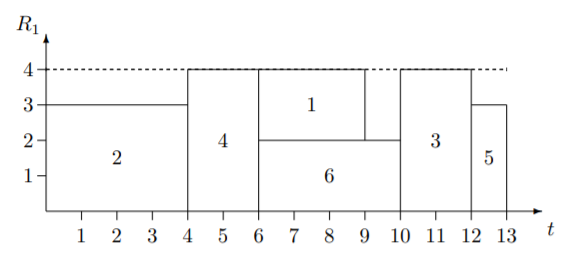
\includegraphics[width=0.8\textwidth]{assets/img/02_Grundlagen/ExampleProjectRCPSP_Schedule.png}
    \caption{Möglicher Zeitplan zum \ac{rcpsp} Beispiel-Projektplan} 
    \label{img:example_rcpsp_schedule}
    \source{\cite[][S. 2]{kolisch_heuristic_1998}}
\end{figure}
Ein möglicher Zeitplan zu dem Beispiel-Projektplan lässt sich in der Abbildung \ref{img:example_rcpsp_schedule} darstellen. Hierbei werden die Ressourcenanforderungen der Aktivitäten mit Berücksichtigung der Abhängigkeiten auf der Zeitachse gemäß deren Dauer zugeordnet. Die gestrichelte, horizontale Linie entspricht der maximalen Kapazität für die Ressource $K_1$, welche $R_1 = 4$ gleichkommt. Diese darf bei der Zeitplanung nicht überschritten werden. Der Makespan (dt. Zykluszeit) $C_{max} = 13$ des Zeitplans lässt sich über der Belegung der erneuerbaren Ressourcenarten über den Endzeitpunkt der letzten Aktivität $J_{j+1}$ ablesen. \\

Das \ac{rcpsp} wird als eine generalisierte Form des \ac{jsp} angesehen, welches als $\mathcal{NP}$-hartes Problem  klassifiziert wurde \cite[vgl.][S. 2]{kolisch_heuristic_1998}. Konkret bedeutet dies, dass das Finden des besten Zeitplans nur bei einem kleinen Lösungs-raum deterministisch über Bruteforcing möglich ist. Bei komplexeren Lösungsräumen sind jedoch zu viele Möglichkeiten vorhanden, als dass in absehbarer Zeit alle Kombinationen betrachtet werden können. \\
% Nicht-erneuerbare Ressourcen stellen zudem ein weiteres Problem dar, denn ungültige Lösungen können auftreten wenn zu einem Zeitpunkt keine nicht-erneuerbaren Ressourcen mehr zur Verfügung stehen. \\
\\
Für das zugrunde liegende Problem wurden (Meta-)Heuristiken und weitere intelligente Verfahren eingeführt, welche zur Findung von adäquaten Zeitplänen beim \ac{rcpsp} eingesetzt werden können \cite[vgl.][S. 2]{kolisch_heuristic_1998}. Der Fokus dieser Masterarbeit liegt bei den Metaheuristiken, welche im Abschnitt \ref{sec:Metaheuristiken} eingeführt werden.

\subsection{Multi-Mode Problemerweiterung} \label{subsec:MRCPSP_MM}

Das \ac{mrcpsp} basiert grundlegend auf dem \ac{rcpsp} und stellt somit eine Erweiterung des Basisproblems dar. \\

% Einfach

Im \ac{mrcpsp} steht für jede Aktivität $j \in J$ eine Menge von Modi $m \in M_j = \{ 1, ..., m_j \}$ zur Verfügung. Hierbei muss eine Aktivität in einem verfügbaren Modus $m \in M_j$ ausgeführt werden. Folglich liegen die Zeit- und Ressourcenanforderungen nicht  direkt bei den Aktivitäten, sondern bei den Modi. Die Zeitanforderung einer Aktivität $j \in J$ im Modus $m \in M_j$ wird über $d_{j,m}$ angegeben. Bei den verfügbaren Ressourcenarten kommen neben den erneuerbaren Ressourcenarten $K = \{1, ..., R\}$ auch nicht-erneuerbare Ressourcenarten $L = \{1, ..., C\}$ hinzu, welche über die Modi der Aktivitäten konsumiert werden. Die Menge an nicht-erneuerbaren Ressourcen stehen wie die erneuerbaren Ressourcen nur in limitierter Anzahl $C_l \in \mathbb{N}$ zur Verfügung. Die Ressourcenanforderungen einer Aktivität $j \in J$ im Modus $m \in M_j$ wird bei erneuerbaren Ressourcenarten über $r_{j,m,k}$ und bei nicht-erneuerbaren Ressourcenarten über $c_{j,m,l}$ angegeben. \cite[vgl.][S. 596 ff.]{wuliang_improved_2014} \\ 

Das Ziel des \ac{mrcpsp} ist identisch mit dem des \ac{rcpsp} und befasst sich ebenfalls mit dem Finden eines Zeitplans mit der minimalsten Projektausführungsdauer. Aufgrund der Problemerweiterung gegenüber dem \ac{rcpsp} sind zudem Anpassungen in der Zielfunktion erforderlich, welche \cite[vgl.][S. 597]{wuliang_improved_2014} aufführt: 
\begin{align}
    \min \, F_{n+1} = \min \, C_{max} & \qquad \textit{es muss gelten:} \label{align:mrcpsp_goal} \\
    \forall j \in J:\, & \sum_{m \in M_j} x_{j,m} = 1 \label{align:mrcpsp_constraint1}\\
    \forall j \in J, h \in P_j:\, & F_h \leq  F_j - \sum_{m \in M_j} x_{j,m} \cdot d_{j,m} \label{align:mrcpsp_constraint2} \\
    \forall k \in K, t \geq 0:\, & \sum_{j \in A(t)} \sum_{m \in M_j} x_{j,m} \cdot r_{j,k} \leq R_k  \label{align:mrcpsp_constraint3}
    \\
    \forall l \in C, t \geq 0:\, & \sum_{j \in J} \sum_{m \in M_j} x_{j,m} \cdot c_{j,l} \leq C_l  \label{align:mrcpsp_constraint4} 
\end{align}
$x_{j,m}$ stellt hierbei eine Entscheidungsvariable dar, die angibt, ob ein Modus $m \in M$ für die Aktivität $j \in M$ selektiert wurde. Sofern dies der Fall ist, entspricht $x_{j,m} = 1$, andernfalls $x_{j,m} = 0$. Die Beschränkung in \ref{align:mrcpsp_constraint1} nutzt diese Entscheidungsvariable, um sicherzustellen, dass für jede Aktivität immer ein Modus ausgewählt wurde. Die Beschränkung aus  \ref{align:mrcpsp_constraint2} stellt die Erweiterung aus \ref{align:rcpsp_constraint1} dar und soll weiterhin sicherstellen, dass die Abhängigkeitsbeziehungen zwischen den Aktivitäten für alle ausgewählten Modis eingehalten werden. \ref{align:mrcpsp_constraint3} berücksichtigt ebenfalls nun die Modusauswahl und stellt sicher, dass die Kapazität an erneuerbaren Ressourcen zu keinem Zeitpunkt überschritten werden darf. Die Beschränkung aus \ref{align:mrcpsp_constraint4} stellt sicher, dass zu keinem Zeitpunkt mehr nicht-erneuerbare Ressourcen konsumiert werden, als zur Verfügung stehen. \\

\begin{figure}[H]
    \centering
    \noindent\makebox[\textwidth]{%
    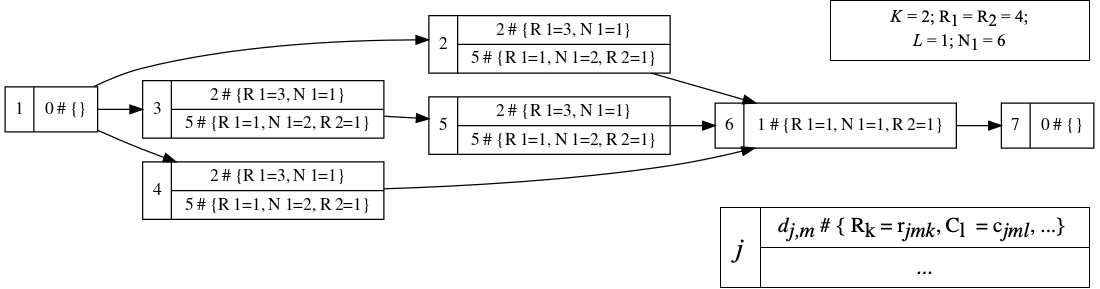
\includegraphics[width=1.1\textwidth]{assets/img/02_Grundlagen/ExampleProjectMRCPSP_Plan.png}
    }
    \caption{Graphen-Darstellung eines \ac{mrcpsp} Beispiel-Projektplans mit $|J| = 7$ Aktivitäten} 
    \label{img:example_mrcpsp}
    \source{Eigene Darstellung}
\end{figure}

Abbildung \ref{img:example_mrcpsp} zeigt eine grafische Darstellung eines \ac{mrcpsp} Beispielprojektes mit 7 Aktivitäten dar, wobei $J_0$ und $J_7$ die Dummy-Knoten entsprechen. Innerhalb der Aktivitätsknoten befinden sich zudem die zugehörigen ausführbaren Modi mit deren Zeit- und Ressourcenanforderungen. Die Aktivitäten $J_2 \, ... \, J_4$ können jeweils in zwei verschiedenen Versionen ausgeführt werden, sofern die Beschränkungen eingehalten werden. \\

\begin{figure}[H]
    \centering
    \noindent\makebox[\textwidth]{%
    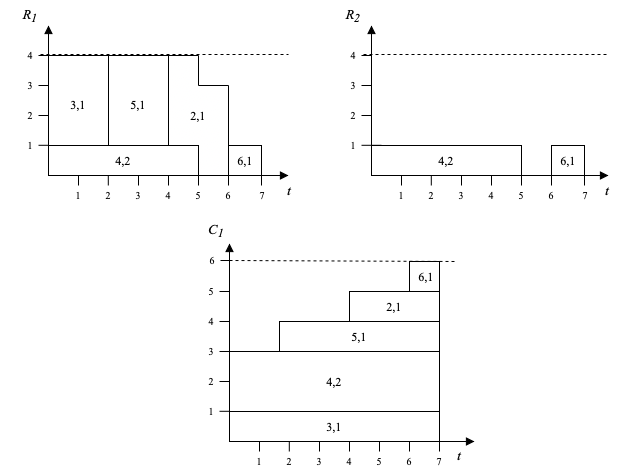
\includegraphics[width=1.1\textwidth]{assets/img/02_Grundlagen/ExampleProjectMRCPSP_Schedule.png}
    }
    \caption{Möglicher Zeitplan zum \ac{mrcpsp} Beispiel-Projektplan} 
    \label{img:example_mrcpsp_schedule}
    \source{Eigene Darstellung}
\end{figure}

Abbildung \ref{img:example_mrcpsp_schedule} zeigt für den \ac{mrcpsp} Beispiel-Projektplan eine optimale Belegung aller Ressourcenarten auf. In der Grafik wurden für alle Aktivitäten auch die zugehörigen Modi gekennzeichnet. Der Makespan für diesen (optimalen) Zeitplan liegt bei $C_{max} = 7$. Dadurch, dass sich nicht-erneuerbare Ressourcen $C_l$ nicht regenerieren, wird dieses Verhalten bei der Ressourcenbelegungsabbildung dahingehend berücksichtigt, dass jede gestartete Aktivität bis zum Projektende andauert. Es lässt sich erkennen, dass für das Beispiel am Projektende keine nicht-erneuerbaren Ressourcen mehr zur Verfügung stehen und folglich das Ausführen von weiteren Aktivitäten über den zweiten Modus zu invaliden Schedules führen würde. Der Verbrauch von nicht-erneuerbaren Ressourcen wäre im zweiten Modus bei allen Aktivitäten im Beispiel-Projektplan höher als bei dem ersten Modus und folglich würde die Grenze $C_l$ überschritten werden. \\
Aufgrund der nicht-erneuerbaren Ressourcenanforderungen und der Möglichkeit, Aktivitäten über verschiedene Modis auszuführen bewies \cite[S. 3 f.]{kolisch_local_1997}, dass sich das \ac{mrcpsp} nicht um ein $\mathcal{NP}$-hartes, sondern sogar um ein $\mathcal{NP}$-vollständiges Problem handelt. Dies ist dann der Fall, wenn mehr als zwei nicht-erneuerbare Ressourcenarten $|L| \geq 2$ und nicht-Dummy Aktivitäten in mehr als zwei Modi $\exists j \in J \, / \, \{ J_0, J_{j+1} \}: |M_j| \geq 2$ ausgeführt werden können \cite[vgl.][S. 3 f.]{kolisch_local_1997}. Durch die Auswahl der Modi wird direkt der Verbrauch an nicht-erneuerbaren Ressourcen beeinflusst. Die nicht-erneuerbaren Ressourcenanforderungen können nach Selektion der Modi die verfügbare Kapazität $C_l$ überschreiten, was ein Schedule gemäß Bedingung \ref{align:mrcpsp_constraint4} ungültig macht. \\

Heuristiken basierend auf prioritätsbasierten Regeln stellen für die Berechnung von Schedules auch beim \ac{mrcpsp} eine wichtige Technik für das Finden von adäquaten, wenn aber nicht optimalen Lösungen dar. Diese werden im Abschnitt \ref{subsec:SGS} genauer beleuchtet. Bei komplexen Projekten mit mehr als 20 Aktivitäten kommen Heuristiken an ihre Grenzen. Folglich werden Metaheuristiken eingesetzt, welche mittels lokaler Suche versuchen die optimale Lösung zu finden. Viele Metaheuristiken benötigen initiale Lösungen, wofür Heuristiken jedoch eine gute Basis darstellen. \cite[vgl.][S. 69 f.]{lova_multi-mode_2006} 
\subsection{Serial Schedule Generation Scheme} \label{subsec:SGS}

\acp{sgs} stellen für das (M)\ac{rcpsp} wesentliche Techniken zur Erzeugung von Zeitplänen dar. Die am häufigsten in der Literatur verwendeten \acp{sgs} sind \acfp{ssgs} und \acfp{psgs}. Das Prinzip eines \ac{sgs} liegt darin,  vollständige Zeitpläne inkrementell über partielle Zeitpläne aufzubauen. Ein partieller Schedule entspricht einem Zeitplan, welcher unvollständig ist und nicht alle Aktivitäten berücksichtigt, sondern nur eine Teilmenge von Aktivitäten. \cite[vgl.][S. 3 f.]{kolisch_heuristic_1998}\\

Die beiden \ac{sgs} Varianten unterscheiden sich bei der Inkrementierungsweise voneinander. Beim \ac{ssgs} werden $n$ Phasen durchlaufen, wobei in jeder Phase eine Aktivität selektiert wird. Bei dem \ac{psgs} werden bis zu $n$ Phasen durchlaufen. Zu jedem Aktivitätsendzeitpunkt wird überprüft, welche Aktivitäten ausgewählt werden können. Während das \ac{ssgs} aktivitätsinkremental funktioniert, agiert das \ac{psgs} zeitinkremental. \cite[vgl.][S. 3 f.]{kolisch_heuristic_1998}\\

Im Rahmen der Masterthesis wird vermehrt das \ac{mrcpsp} behandelt, welches in Kombination mit dem \acf{psgs} nicht immer eine optimale Lösung darstellt \cite[vgl.][S. 911 f.]{alcaraz_solving_2003} \cite[vgl.][S. 5 f.]{kolisch_heuristic_1998} . Folglich beschränkt sich diese Arbeit auf das \ac{ssgs}. 

\begin{lstlisting}[caption={\ac{ssgs}-Algorithmus (Quelle: \cite[S. 3]{kolisch_heuristic_1998}}), label=lst:sgsalgorithm, mathescape=true, inputencoding={utf8}, extendedchars=false, escapeinside=``]
Init: $F_0$, $S_0 = $ {0},
for g = 1 to n do
    Berechne $\mathcal{D}_g, \mathcal{F}_g, \tilde{\mathcal{R}}_k(t) \, (k \in \mathcal{K}; t \in \mathcal{F}_g)$ 
    W`ä`hle ein $j \in \mathcal{D}$ aus
    $EFT_j$ = $\max_{h \in \mathcal{P}_j} \{ F_h \} + p_j$
    $F_j$ = $\min \{ t \in [EFT_j - p_j, LFT_j - p_j] \cap \mathcal{F}_g | r_{j,k} \leq R_k(\tau), k \in \mathcal{K}, \tau \in [t, t + p_j [\cap \mathcal{F}_g\} + p_j $
    $\mathcal{S}_g$ = $\mathcal{S}_{g - 1} \cup \{ j \}$
$F_{n+1}$ = $\max_{h \in \mathcal{P}_{n+1}} \{ F_h \}$  
\end{lstlisting}

Listing \ref{lst:sgsalgorithm} stellt den \ac{ssgs}-Algorithmus aus dem Manuskript von \cite{kolisch_heuristic_1998} dar. Hierbei wird in jeder Phase $g$ die Mengen $\mathcal{S}_g$ und $\mathcal{D}_g$ berechnet. Die Menge $\mathcal{S}_g$ beinhaltet bereits berücksichtigte Aktivitäten, während $\mathcal{D}_g$ die selektierbaren Aktivitäten für die Phase $g$ beinhaltet. Die Menge $\mathcal{F}_g$ beinhaltet zu $\mathcal{S}_g$ die Endzeiten der einzelnen Aktivitäten. $\tilde{\mathcal{R}}_k(t)$ gibt die Anzahl noch verfügbarer erneuerbarer Ressourcen für die Ressourcenart $k$ zum Zeitpunkt $t$ an. \cite[vgl.][S. 3 f.]{kolisch_heuristic_1998}\\

Abbildung \ref{img:example_ssgs_application} zeigt auf, wie \ac{ssgs} auf einen Projektplan angewendet werden kann, um eine mögliche Lösung für das \ac{rcpsp} zu erhalten. Die Auswahl der Aktivität $j$ aus $\mathcal{D}_g$ erfolgte in dem Beispiel willkürlich. 

\begin{figure}[H]
    \centering
    \noindent\makebox[\textwidth]{%
    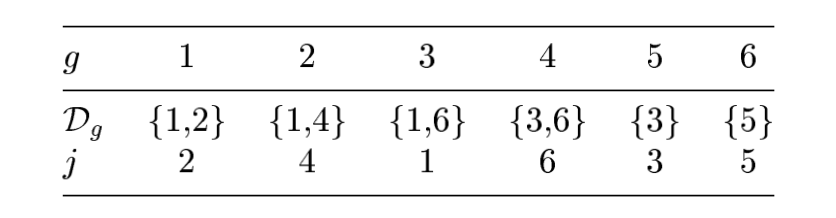
\includegraphics[width=0.6\textwidth]{assets/img/02_Grundlagen/ExampleSSGS.png}
    }
    \caption{\acs{ssgs}-Anwendung auf den RCPSP Beispiel-Projektplan von Abbildung \ref{img:example_rcpsp} zur Erstellung des Zeitplans aus Abbildung \ref{img:example_rcpsp_schedule}}
    \label{img:example_ssgs_application}
    \source{\cite[vgl.][S. 3]{kolisch_heuristic_1998}}
\end{figure}

Aus dem Listing \ref{lst:sgsalgorithm} heraus lassen sich weitere Kennziffern von Aktivitäten innerhalb eines Projektplans erkennen. Im Algorithmus wurden \ac{EFT} und \ac{LFT} verwendet. Diese und \ac{EST} und \ac{LST} sind wesentlich für viele prioritätsbasierte Aktivitätsregeln (vgl. Abschnitt \ref{subsec:SGS_Aktivitaeten}) und für die Robustheitsberechnungen (vgl. Abschnitt \ref{subsec:Praediktive_Methoden}) und werden in der Tabelle \ref{tab:cmr_kennziffern} eingeführt. \\

\begin{table}[H]
\centering
\begin{adjustbox}{width=0.9\columnwidth,center}
\begin{tabular}{|l|l|l|}
\hline
Abk. & Beschreibung \cite[vgl.][S. 126]{burke_project_1999} & Formel \cite[vgl.][S. 127 ff.]{burke_project_1999} \\ \hline
EST  & \begin{tabular}[c]{@{}l@{}}Earliest Starting Time\\ (dt. frühster Startzeitpunkt)\\ stellt den frühstmöglichen Start-\\ zeitpunkt einer Aktivität $j$ dar. \end{tabular}  & $EST_j = \max_{h \in P(j)} \{ EFT(h) \}$ \\ \hline
EFT  & \begin{tabular}[c]{@{}l@{}}Earliest Finishing Time\\ (dt. frühster Endzeitpunkt) \\ stellt den frühstmöglichen End-\\ zeitpunkt einer Aktivität $j$ dar. \end{tabular} & $EFT_j = EST_j + d_j $\\ \hline
LST  & \begin{tabular}[c]{@{}l@{}}Latest Starting Time\\ (dt. spätester Startzeitpunkt)\\ stellt den spätesten Startzeit-\\ punkt einer Aktivität $j$ dar, ohne \\ dass das Projekt in Verzug kommt. \end{tabular} & $LST_j = LFT_j - d_j$ \\ \hline
LFT  & \begin{tabular}[c]{@{}l@{}}Latest Finishing Time\\ (dt. spätester Endzeitpunkt)\\ stellt den spätesten Endzeit-\\ punkt einer Aktivität $j$ dar,\\ ohne dass das Projekt in \\ Verzug kommt. \end{tabular}  & $LFT_j = \min_{h \in P(j)} \{ LST(h) \}$ \\ \hline
\end{tabular}
\end{adjustbox}
\caption{Kennziffern der kritischen Pfadmethode}
\source{In Anlehnung an \cite{burke_project_1999}}
\label{tab:cmr_kennziffern}
\end{table}

\subsubsection{Aktivitäts- und Moduslisten} \label{subsec:SGS_Darstellung}  
Aktivitäts- und Moduslisten sind wesentliche Techniken zur Repräsentation von Lösungen für das (M)\ac{rcpsp}. Insbesondere Metaheuristiken nutzen diese Art der Repräsentation, um aus den Listen Zeitpläne zu transferieren \cite[vgl.][S. 10]{rezaeian_using_2015}, \cite[vgl.][S. 602]{wuliang_improved_2014}, \cite[vgl.][S. 2370]{li_solving_2013}. \\

Zeitpläne im \ac{rcpsp} lassen sich über Aktivitätslisten  $\lambda = \langle j_1, j_2, ..., j_n \rangle$ darstellen. Die Reihenfolge der Aktivitäten entspricht die der Planungsreihenfolge. Folglich müssen die Abhängigkeiten der Aktivitäten zueinander innerhalb der Aktivitätsliste $\lambda$ eingehalten werden. Im Beispiel der Abbildung \ref{img:example_rcpsp_schedule} entspricht die Aktivitätsliste $\lambda = \langle 2, 4, 1, 6, 3, 5 \rangle$. \cite[vgl.][S. 3 f.]{kolisch_heuristic_1998} \\

Für das \ac{mrcpsp} müssen zudem Modi der zugehörigen Aktivitäten berücksichtigt werden. Hierfür werden zusätzlich zu den Aktivitätslisten auch Moduslisten eingesetzt. Eine Modusliste $\mu = \langle m_1, m_2, ..., m_n \rangle$ berücksichtigt ebenfalls die Planungsreihenfolge. Die Länge der Modusliste entspricht der Länge der Aktivitätsliste $|\mu| \equiv |\lambda|$. Folglich können über Aktivitäts- und Moduslisten die Aktivitäten und Modi über die Positionierung zugeordnet werden \cite[vgl.][S. 908]{sebt_efficient_2015}. Für das Beispiel aus Abbildung \ref{img:example_mrcpsp_schedule} entspricht die Aktivitäts- und Modusliste das Tupel $(\lambda, \mu) = (\langle 1, 3, 4, 5, 2, 6, 7 \rangle, \langle 1, 1, 2, 1, 1, 1, 1 \rangle)$. Abbildung \ref{img:ActivityModeListExample} illustriert dieses Beispiel. \\

\begin{figure}[H]
    \centering
    \noindent\makebox[\textwidth]{%
    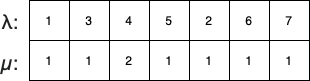
\includegraphics[width=0.45\textwidth]{assets/img/02_Grundlagen/ActivityModeListExample.png}
    }
    \caption{Darstellung der Aktivitäts- und Modusliste $(\lambda, \mu)$ für das MRCPSP Beispiel-Projektplan} 
    \label{img:ActivityModeListExample}
    \source{Eigene Darstellung}
\end{figure}

Eine Lösung für das \ac{mrcpsp} entspricht dem Tupel $I = (\lambda, \mu)$. Für jeden Projektplan existiert mindestens eine optimale Lösung mit der kürzesten Projektdauer $I^* = (\lambda^*, \mu^*)$ \cite[vgl.][S. 4]{kolisch_heuristic_1998}. Das Ziel der (Meta-)Heuristiken liegt darin, die optimale Lösung $I^*$ zu finden oder dieser zumindest sehr nahezukommen. Hierfür müssen Aktivitäts- und Moduslisten ausgewählt, evaluiert und anschließend weitergesucht werden. Abschnitt \ref{subsec:SGS_Aktivitaeten} befasst sich mit Heuristiken zum Finden von Aktivitätslisten, Abschnitt \ref{subsec:SGS_Modi} mit dem Finden von Moduslisten. 

\subsubsection{Prioritätsbasierte Regeln für Aktivitäten} \label{subsec:SGS_Aktivitaeten}

Das \acl{ssgs} stellt eine bedeutende Technik zur Erzeugung von Aktivitätslisten dar. Hierbei wird in jeder Phase $g$ eine Aktivität $j$ aus den möglichen Aktivitäten $\mathcal{D}_g$ ausgewählt. Die Auswahl der Aktivität $j \in \mathcal{D}_g$ gilt es mittels prioritätsbasierten Regeln zu bestimmen. \cite[vgl.][S. 5]{kolisch_heuristic_1998}\\

Prioritätsbasierte Regeln bestehen aus zwei Komponenten, nämlich einer Prioritätswertfunktion $v(j)$ und einem Auswahlparameter $extr$. Die Prioritätswertfunk-tion für Aktivitäten ist über $v: \mathcal{D}_g \rightarrow \mathbb{R}_0$ gemappt und wird über die Prioritätsregeln definiert. Die Funktion gibt für eine mögliche Aktivität $j \in \mathcal{D}_g$ den entsprechenden Prioritätswert gemäß der Regel an. Der Auswahlparameter $extr \in \{ \text{MIN}, \text{MAX} \}$ bestimmt das Extremum. In jeder Phase wird eine Aktivität ausgewählt, die mit dem zugehörigen Prioritätswert dem Extremum aller möglichen Aktivitäten entspricht. Sofern mehrere Aktivitäten dem Extremwert entsprechen, muss eine weitere Heuristik eingeführt werden, wie die Auswahl über die geringste Aktivitätsnummer. \cite[vgl.][S. 6 f.]{schirmer_parameterized_1997}

% Beispiel Auswahl über Prioritätswert

\begin{table}[H]
\centering
\begin{tabular}{r|lll}
Abkürzung & Name & \multicolumn{1}{c}{\begin{tabular}[c]{@{}c@{}}Prioritätsregel-\\funktion $v(j)$\end{tabular}} & \multicolumn{1}{c}{\begin{tabular}[c]{@{}c@{}}Auswahl-\\parameter $extr$\end{tabular}} \\ \hline
GRPW & Greatest Rank Positional Weight & $d_j + \sum_{i \in S(j)} d_i $ & MAX \\
LFT & Latest Finish Time & $LFT_j $ & MIN \\
LST & Latest Start Time & $LST_j $ & MIN \\
MSLK & Minimum Slack & $LFT_j - EFT_j$ & MIN \\
MTS & Most Total Successors & $|S(j)| $ & MAX \\
\end{tabular}
\caption{Prioritätsregeln für Aktivitäten}
\label{tab:ActivityRules}
\source{\cite[vgl.][S. 6]{kolisch_heuristic_1998}}
\end{table}

Die in Tabelle \ref{tab:ActivityRules} aufgeführten etabilierten Regeln werden genutzt, um anhand der Prioritätsregelfunktion $v(j)$ gemäß Auswahlparameter $extr$ die zugehörige Aktivität $j$ auszuwählen. Tabelle \ref{tab:ActivityRulesExample} zeigt ein Beispiel bei Anwendung einer beliebigen Prioritätsregelfunktion $v(j)$ auf. Sofern der Auswahlparameter $extr = \text{MAX}$ entspricht, wird in der Phase $g$ die Aktivität 3 ausgewählt, bei $extr = \text{MIN}$ die Aktivität 2.  
 
\begin{table}[H]
\centering
\begin{tabular}{r|c|c|c|c}
$j \in \mathcal{D}_g$ & 1 & 2 & 3  & 4 \\ \hline
$v(j)$ & 5 & 3 & 12 & 4
\end{tabular}
\caption{Beispiele von Prioritätswerten von den möglichen Aktivitäten $j \in \mathcal{D}_g$ einer Phase $g$}
\label{tab:ActivityRulesExample}
\source{Eigene Darstellung}
\end{table}


\subsubsection{Selektionsregeln für Modi} \label{subsec:SGS_Modi}
Um beim \ac{mrcpsp} Zeitpläne zu erzeugen, müssen neben den Aktivitätslisten auch Moduslisten generiert werden. Des Weiteren besteht beim \ac{mrcpsp} die Problematik, dass bei Anwendung der Prioritätsregeln für eine Aktivität mehrere Modi mit unterschiedlichen Ressourcen- und Zeitanforderungen zur Verfügung stehen. Folglich werden Selektionsregeln für Modi benötigt, welche analog zu den Prioritätsregeln für Aktivitäten funktionieren. \\


\begin{table}[H]
\centering
\resizebox{\textwidth}{!}{%
\begin{tabular}{r|lll}
Abkürzung & Name & \multicolumn{1}{c}{\begin{tabular}[c]{@{}c@{}}Selektionsregel-\\funktion $s(j, m)$\end{tabular}} & \multicolumn{1}{c}{\begin{tabular}[c]{@{}c@{}}Auswahl-\\parameter $extr$\end{tabular}} \\ \hline
LPSRD & Least Product Sum of Res. and Dur. & $\sum_{l=1}^{|L|} (c_{j,m,l} \cdot d_{j,m})$ & MIN \\
LRP & Least Resource Proportion & $\max (\frac{r_{j,m,k}}{|K|})$ & MIN \\
LRS & Least Sum of Non-renewable Resource & $\sum_{l=1}^{|L|}  \frac{c_{j,m,l}}{R^v_k}$ & MIN \\
LTRU & Least Total Resource Usage & $\sum_{l=1}^{|L|} c_{j,m,l}$ & MIN \\
SFM & Shortest Feasible Mode & $d_{j,m}$ & MIN \\

\end{tabular}
}%
\caption{Selektionsregeln für Modi}
\label{tab:ModeRules}
\source{\cite[vgl.][S. 5046]{chen_entropy-based_2014}}
\end{table}

Die in Tabelle \ref{tab:ModeRules} aufgeführten etabilierten Regeln werden genutzt, um anhand der Selektionsregelfunktion $s(j, m)$ gemäß Auswahlparameter $extr$ den zugehörigen Modus $m \in M_j$ einer Aktivität $j$ auszuwählen. Tabelle $\ref{tab:ModesRulesExample}$ zeigt ein Beispiel bei Anwendung einer beliebigen Prioritätsregelfunktion $v(j)$ und Selektionsregelfunktion $s(j, m)$ auf. Um die Aktivitätsregelfunktion anwenden zu können, müssen vorher die Modi selektiert werden \cite[vgl.][S. 5046]{chen_entropy-based_2014}. Die Selektion der Modi und Aktivitäten geschieht im Beispiel über $extr = \text{MAX}$. Für alle möglichen Aktivitäten der Phase $j \in \mathcal{D}_g$ wird somit der erste Modus ausgewählt. Im Anschluss können die Aktivitäten über die Prioritätsregeln ausgewählt werden (vgl. Abschnitt \ref{subsec:SGS_Aktivitaeten}). 


\begin{table}[H]
\centering

\begin{tabular}{r|cc|cc|cc|cc}
$j \in \mathcal{D}_g$  & \multicolumn{2}{c|}{1} & \multicolumn{2}{c|}{2} & \multicolumn{2}{c|}{3} & \multicolumn{2}{c}{4} \\ \hline
$m \in M_j$ & \multicolumn{1}{c|}{1} & 2 & \multicolumn{1}{c|}{1} & 2 & \multicolumn{1}{c|}{1} & 2 & \multicolumn{1}{c|}{1} & 2 \\ \hline
$s(j, m)$                 & \multicolumn{1}{c|}{5} & 3 & \multicolumn{1}{c|}{2} & 1 & \multicolumn{1}{c|}{5} & 4 & \multicolumn{1}{c|}{7} & 7 \\ \hline
$v(j)$                      & \multicolumn{2}{c|}{5} & \multicolumn{2}{c|}{3} & \multicolumn{2}{c|}{12} & \multicolumn{2}{c}{2} 
\end{tabular}%

\caption{Beispiele von Prioritäts- und Selektionswerten von den möglichen Aktivitäten $j \in \mathcal{D}_g$ und Modis der Aktivitäten einer Phase $g$}
\label{tab:ModesRulesExample}
\source{Eigene Darstellung}
\end{table}

\subsubsection{Sampling als Multi Pass Methode} \label{subsec:SGS_RBBRS}

Das Anwenden der Aktivitäts- und Modusregeln führt innerhalb eines \ac{ssgs} zu einem einzigen Zeitplan und wird somit als eine Single Pass Methode klassifiziert \cite[vgl.][S. 6]{kolisch_heuristic_1998}. Das Anwenden dieser Heuristiken führt bei gleichbleibendem Input zudem immer zu identischen Ergebnissen und sind folglich deterministisch \cite[vgl.][S. 4]{schirmer_parameterized_1997}. Dennoch besteht das Interesse eine breitere Menge an möglichen Zeitplänen zu untersuchen, um durchaus bessere Ergebnisse als das direkte Anwenden der Regeln zu erhalten.\\

Unter Multi Pass Methoden werden wiederum Verfahren bezeichnet, die in der Lage sind, mehrere Zeitpläne zu generieren. Hierunter fallen Verfahren, wie das Anwenden von mehreren Regeln, aber auch das Sampling. Für jede mögliche Aktivität einer Phase $j \in \mathcal{D}_g$ und deren jeweiligen Modi $m \in M_j$ ist hierbei ein Wahrscheinlichkeitswert gemäß Funktion $p(x) \in [0, 1]$ vorgesehen, welche für die Entscheidungsmenge aufkommuliert stets 1 ergeben muss. Aus der Entscheidungsmenge wird im Anschluss gemäß der Wahrscheinlichkeit die Aktivität bzw. der Modus ausgewählt. Die Wahrscheinlichkeitsfunktion $p(x)$ wird anhand von Sampling Methoden definiert. \cite[vgl.][S. 7 f.]{kolisch_heuristic_1998} Aufgrund der Einfachheit beziehen sich die Formeln der folgenden vorgestellten Sampling Methoden nur auf die Aktivitätsauswahl. Diese lassen sich jedoch ohne weiteres auch auf die Modusauswahl ableiten. \\

Die einfachste Sampling Methode ist \ac{RS}. Hierbei ist die Wahrscheinlichkeit $p(x)$ innerhalb der Entscheidungsmenge gleichverteilt $p(j) = \dfrac{1}{|\mathcal{D}_g|}$. \cite[vgl.][S. 7]{kolisch_heuristic_1998} Hierbei werden Prioritäts- und Selektionregeln ignoriert und gänzlich zufällige Zeitpläne erzielt. \\

Eine weitere Sampling Methode ist \ac{BRS}. Die Wahrscheinlichkeit $p(x)$ hängt hierbei direkt von der Prioritäts- und Selektionsregel ab $p(j) = \dfrac{v(j)}{\sum_{i \in \mathcal{D}_g} v(i)}$. \cite[vgl.][S. 7]{kolisch_heuristic_1998} \\

Über \ac{RBRS} ist es zudem möglich, die Wahrscheinlichkeit $p(x)$ über einen Regretwert (dt. Reuewert) zu beeinflussen \cite[vgl.][S. 12]{schirmer_parameterized_1997}. Dies führt dazu, dass die Aktivitäts- und Moduslisten gemäß der Prioritäts- und Selektionsregeln mehr oder weniger variieren können. Die Wahrscheinlichkeit $p(x)$ lässt sich über die folgenden Funktionen gemäß \cite[vgl.][S. 12]{schirmer_parameterized_1997} definieren: 
\begin{align}
    v'(j) &= 
    \left\{\begin{array}{ll} 
        \max_{i \in \mathcal{D}_n}(v(i)) - v(j) & \text{wenn extr = min} \\
        v(j) - \min_{i \in \mathcal{D}_n}(v(i)) & \text{wenn extr = max} \\
     \end{array}\right.  \\
    v''(j) &= (v'(j) + \epsilon)^\alpha  \\
    p(j) &= \frac{v''(j)}{\sum_{i \in D_n} v''(i)}
\end{align}

$v'(j)$ und $v''(j)$ stellen die Regrets dar. Beim \ac{RBRS} werden die Regrets zudem mit $\epsilon = \mathbb{R}_{>0}$ und $\alpha = \mathbb{R}_{\geq0}$ parametrisiert. $\epsilon$ garantiert, dass $v''(j) \neq 0$. Dies ist relevant, um innerhalb der Wahrscheinlichkeitsfunktion $p(x)$ Divisionen durch 0 zu vermeiden. $\alpha$ regelt den Einfluss der Prioritäts- und Selektionsregelfunktion auf den Wahrscheinlichkeitswert. Bei einem hohen Wert verstärkt sich der Einfluss, bei einem niedrigen Wert verringert sich dieser. Bei $\alpha = 0$ ist die Prioritäts- und Selektionsregelfunktion irrelevant und folglich sind die Wahrscheinlichkeiten innerhalb der Entscheidungsmenge gleichverteilt, identisch zum \ac{RS}. Bei $\alpha = \infty$ sind die Wahrscheinlichkeiten so angeordnet, dass die Aktivität oder der Modus deterministisch ausgewählt werden kann, identisch zur Single Pass Methode. \cite[vgl.][S. 12 f.]{schirmer_parameterized_1997} \\

Die Funktionsweise der vorgestellten Multi Pass Samplingverfahren lassen sich in Tabelle \ref{tab:ExampleSampling} aufbauend auf dem Beispiel aus Abschnitt \ref{subsec:SGS_Aktivitaeten} verdeutlichen. Für dieses Beispiel liegt der Extremwert für die zu betrachtende Prioritätsregel bei $extr = \text{MAX}$. Sofern \ac{RBRS} als Sampling-Methode ausgewählt wurde, so wird z. B. die Aktivität 3 mit einer 80 prozentigen Wahrscheinlichkeit selektiert. Wenn $\alpha = \infty$, dann wird das Ergebnis gemäß der regelbasierten Single Pass Methode deterministisch ausgewählt.  




\begin{table}[H]
\centering
\begin{tabular}{r|l|l|l|l}
$j \in \mathcal{D}_g$                      & \multicolumn{1}{c|}{1} & \multicolumn{1}{c|}{2} & \multicolumn{1}{c|}{3}  & \multicolumn{1}{c}{4} \\ \hline
$v(j)$                                     & \multicolumn{1}{c|}{5} & \multicolumn{1}{c|}{3} & \multicolumn{1}{c|}{12} & \multicolumn{1}{c}{4} \\ \Xhline{2\arrayrulewidth}
\acf{RS} & 0.25                   & 0.25                   & 0.25                    & 0.25                  \\ \hline
\acf{BRS}& 0,21                   & 0,13                   & 0,50                    & 0,16                  \\ \hline
\acf{RBRS} & 0,10                   & 0,03                   & 0,80                    & 0,07                  \\ \hline
\ac{RBRS} mit $\alpha = 0$                      & 0.25                   & 0.25                   & 0.25                    & 0.25                  \\ \hline
\ac{RBRS} mit $\alpha = \infty$                      & 0.00                   & 0.00                   & 1.00                    & 0.00                 
\end{tabular}
\caption{Selektionswahrscheinlichkeiten $p(j)$ für die vorgestellten Sampling-Verfahren mit $|\mathcal{D}_g| = 4$ und $extr = \text{MAX}$ }
\label{tab:ExampleSampling}
\source{In Anlehnung an \cite[vgl.][S. 8]{kolisch_heuristic_1998}}
\end{table}

\subsection{Unsicherheiten} \label{subsec:MRCPSP_Unsicherheiten}

Insbesondere in der Realität ist es möglich, dass Unsicherheiten auftreten können. Dies kann der Fall sein, wenn Events, wie der Ausfall von Maschinen, die Erkrankung von Mitarbeitern, die Fehleinschätzung bei der Planung usw. auftreten \cite[vgl.][S. 64 ff.]{deblaere_reactive_2011}. Durch Verspätungen können Projekte in Verzug kommen und somit die geplante Makespan $C_{max}$ überschreiten. Dies ist suboptimal und stellt eine Herausforderung bei der Erzeugung von Zeitplänen dar. Mit solchen Unsicherheiten gilt es auf abstrakter Ebene innerhalb des (M)RCPSP umzugehen. \\

Es können verschiedene Arten von Unsicherheiten betrachtet werden. Die in der Literatur am häufigsten aufzufindenden Unsicherheitsarten sind Verspätungen von Aktivitäten und erneuerbaren Ressourcen, die nicht zu jedem Zeitpunkt konstant vorliegen. \cite[vgl.][S. 64 ff.]{deblaere_reactive_2011} \\

Störungen der Aktivitätsdauer treten auf, wenn die tatsächliche Dauer einer Aktivität größer ist, als die geplante Dauer $d_j$. Die Differenz zwischen geplanter und tatsächlicher Dauer wird über $\Delta_j \in \mathbb{N}$ ausgedrückt. \cite[vgl.][S. 65]{deblaere_reactive_2011} Dies wird in Abbildung \ref{img:example_mrcpsp_schedule_activitydisturbance} anhand des MRCPSP Beispiel-Zeitplans aus Abschnitt \ref{subsec:MRCPSP_MM} bei der Aktivität 4 mit $\Delta_4$ = 1 deutlich. Zudem lässt sich erkennen, dass der geplante Makespan gegenüber dem initialen Zeitplan (Abbildung \ref{img:example_mrcpsp_schedule}) trotz der Störung nicht in Vorzug kommt, da die Verspätung über den Puffer von einer Zeiteinheit und einer verfügbaren Ressource $R_1$ und mehreren Ressourcen $R_2$ vor Durchlauf der Folgeaktivität bedient werden konnte. 

\begin{figure}[H]
    \centering
    \noindent\makebox[\textwidth]{%
    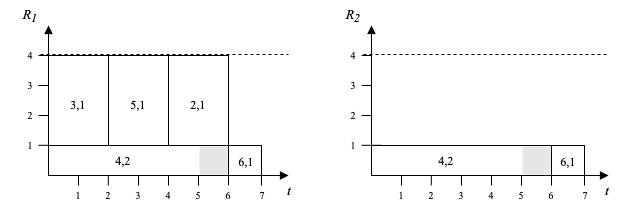
\includegraphics[width=1\textwidth]{assets/img/02_Grundlagen/ExampleProjectMRCPSP_ScheduleDelay.drawio.png}
    }
    \caption{MRCPSP Beispiel-Zeitplan mit einer Aktivitätsstörung von $\Delta_4$ = 1} 
    \label{img:example_mrcpsp_schedule_activitydisturbance}
    \source{Eigene Darstellung}
\end{figure}

Eine weitere Art von Unsicherheiten stellen Störungen bei den erneuerbaren Ressourcen dar. Bei dieser Störungsart besteht die Annahme, dass die Anzahl der verfügbaren Ressourcen einer Ressourcenart $R_k$ zu einem Zeitpunkt $t$ über die Differenz $\Delta^\rho_k \in \mathbb{N}$ reduziert wird. Über $t + \delta_t$ wird angegeben, ab welchem Zeitpunkt die erneuerbaren Ressourcenarten wieder komplett zur Verfügung stehen \cite[vgl.][S. 65 f.]{deblaere_reactive_2011}. Abbildung \ref{img:example_mrcpsp_schedule_resourcedisturbance} verdeutlicht die erneuerbaren Ressourcenstörungen. Im Zeitintervall $[4, 7]$ befindet sich eine erneuerbare Ressourcenstörung $\Delta^\rho_1 = 1$. Aktivität 2 kann somit nicht planmäßig ab Zeiteinheit 4 gestartet werden, da durch die Störung nicht genügend erneuerbare Ressourcen für den ausgewählten Modus vorhanden sind. Somit muss entweder ein anderer Modus ausgewählt werden oder solange mit dem Start von Aktivität 2 gewartet werden, bis die erneuerbaren Ressourcen für die komplette Laufzeit der Aktivität wieder zur Verfügung stehen. Der Start der Ausführung wäre bei dem selektierten Modus ab $t = 5$ der Fall, da durch das Fertigstellen von Aktivität 4 eine erneuerbare Ressource $R_1$ freigegeben wird und somit die erforderliche Anzahl von Ressourcen ($r_{2,1,1} = 3$) zur Verfügung stehen. Dadurch kommt jedoch bei Aktivität 6 ein Startverzug von einer Zeiteinheit. Durch diese Störung erhöht sich der Makespan des Zeitplans aus Abbildung \ref{img:example_mrcpsp_schedule_resourcedisturbance} ($C_{max} = 8$) gegenüber dem Zeitplan aus Abbildung \ref{img:example_mrcpsp_schedule} ($C_{max} = 7$) um eine Zeiteinheit.

\begin{figure}[H]
    \centering
    \noindent\makebox[\textwidth]{%
    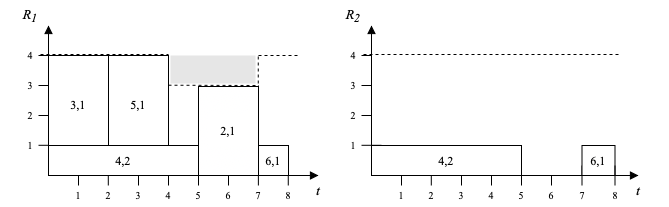
\includegraphics[width=1\textwidth]{assets/img/02_Grundlagen/ExampleProjectMRCPSP_ScheduleResourceDelay.drawio.png}
    }
    \caption{MRCPSP Beispiel-Zeitplan mit einer (erneuerbaren) Ressourcenstörung ab $t$ = 4 von $\Delta_1^\rho$ = 1, welche ab $t + \delta_t = 7$ normalisiert wird} 
    \label{img:example_mrcpsp_schedule_resourcedisturbance}
    \source{Eigene Darstellung}
\end{figure}

Das Ziel des (M)RCPSP besteht darin, den Zeitplan mit der geringsten Projektausführungsdauer zu finden. Der Umgang mit Unsicherheiten stellt zudem eine Herausforderung dar. \cite{brcic_resource_2012} beleuchtete in einer Erhebung einige Möglichkeiten zum Umgang des Unsicherheitsproblems für die stochastische Version des RCPSP. \\

Die naivste Herangehensweise mit Unsicherheiten umzugehen ist es diese bei der Zeitplanerstellung zu ignorieren. Diese Methode wird von \cite{brcic_resource_2012} als prädiktiv bezeichnet. Das Ignorieren von Unsicherheiten kann jedoch dazu führen, dass der Zeitplan durch Verspätungen stärker in Verzug kommt als bei anderen Herangehensweisen. \cite[vgl.][S. 404]{brcic_resource_2012} \\

Die proaktive Herangehensweise behandelt das Problem der Unsicherheiten, indem eine weitere Zielfunktion, nämlich die Robustheit eingeführt wird \cite[vgl.][S. 404]{brcic_resource_2012}. Die Robustheit gibt an, dass der Zeitplan mit geringfügigen Veränderungen (z. B. die der Unsicherheitszenarien) von Aktivitäten umgehen kann \cite[vgl.][S. 246]{khemakhem_efficient_2013}. \\

Die dritte Herangehensweise stellt die reaktiven Methoden dar. Diese reagieren direkt zum Zeitpunkt der Unsicherheit. Hierbei besteht die Möglichkeit, den Zeitplan ab der Unsicherheitsstelle zu reparieren oder gänzlich ab der Stelle der Unsicherheit einen neuen Zeitplan zu erstellen \cite[vgl.][S. 404 f.]{brcic_resource_2012}.  \\

In der Literatur werden prädiktive Verfahren auch als proaktive Verfahren bezeichnet und umgekehrt \cite[vgl.][S. 246]{khemakhem_efficient_2013}. Im Rahmen der Masterarbeit werden folglich die eingangs vorgestellten proaktiven Verfahren nun als prädiktive Verfahren behandelt, welche z. B. die Robustheit optimieren. Die eingangs vorgestellten prädiktiven Verfahren werden somit als proaktive Verfahren angesehen, welche z. B. Unsicherheiten ignorieren. Im Abschnitt  \ref{subsec:Praediktive_Methoden} werden die prädiktiven Methoden, repräsentierend durch die Robustheit,s konkreter vorgestellt. Die reaktiven Methoden, repräsentierend durch das Erzeugen von neuen Zeitplänen zu den Unsicherheitszeitpunkten, werden im Abschnitt \ref{subsec:Reaktive_Methoden} vorgestellt.

\subsubsection{Prädiktive Methoden}
\label{subsec:Praediktive_Methoden}

Eine Möglichkeit mit Unsicherheiten umzugehen stellt das vorausschauende Erstellen von Zeitplänen dar. Hierbei wird neben der Minimierung der Projektdauer $C_{max}$ eine weitere Zielfunktion eingeführt, nämlich die Maximierung der Robustheit $\Omega$. Die Robustheit gilt als die Maßeinheit, wie gut mit kleinen Änderungen innerhalb eines Zeitplans umgegangen werden kann, ohne dass die Projektdauer durch die Verspätung ansteigt \cite[vgl.][S. 246]{khemakhem_efficient_2013} \cite[vgl.][S. 177]{al-fawzan_bi-objective_2005}. \\

Eine mögliche Messung von Robustheit kann über die Summe aller freien Puffer der Aktivitäten definiert werden. Unter einem freien Puffer $s_j$ werden die Zeiteinheiten verstanden, die eingesetzt werden können, damit die unmittelbare Folgeaktivität nicht verzögert wird. Die Einhaltung der Ressourcenbeschränkung muss im Puffer dennoch berücksichtigt werden. Folglich ist die Robustheit über $\Omega = \sum_{j=1}^n s_j$ definiert. \cite[vgl.][S. 177]{al-fawzan_bi-objective_2005} \\

Der freie Puffer lässt sich über die frühsten und spätesten Start- bzw. Endzeitpunkte berechnen $s_j = LST_j - EST_j \Leftrightarrow s_j = LFT_j - EFT_j$. Während $EST_j$ und $EFT_j$ sich über den erstellten Zeitplan ablesen lassen, müssen $LST_j$ und $LFT_j$ über die Backward Recursive Prodecure berechnet werden \cite[vgl.][S. 181]{al-fawzan_bi-objective_2005}. \\

Bei dem \ac{rcpsp} Beispiel-Zeitplan $S^1$ aus Abbildung \ref{img:example_rcpsp_schedule} liegt die Robustheit bei $\Omega^1 = \sum_{j=1}^n s_j = 1$, da der einzige freie Puffer bei Aktivität $j_1$ liegt. Bei einer Verspätung von $\Delta_1 = 1$ würde es zu keiner Verspätung der Projektdauer $C_{max}$ kommen, da der Puffer genutzt werden kann. Sofern es bei einer anderen Aktivität zu einer Verspätung kommt, wird sich die Projektdauer $C_{max}$ verzögern. Ähnlich sieht es bei dem \ac{mrcpsp} Beispiel-Zeitplan $S^2$ aus Abbildung \ref{img:example_mrcpsp_schedule} aus, welcher ebenfalls einen Wert von $\Omega^2 = \sum_{j=1}^n s_j = s_4 = 1$ aufweist. Bei Nutzung des Puffers liegt nach dem Verspätungsszenario $\Delta_4 = 1$ die Robustheit bei $\Omega^{2'} = 0$ (vgl. Abbildung \ref{img:example_mrcpsp_schedule_activitydisturbance}). \\

Ein Zeitplan mit der gleichen Projektdauer $C_{max}$ kann unterschiedliche Robustheitswerte aufweisen und ist folglich für Unsicherheitsszenarien mehr oder weniger geeignet \cite[vgl.][S. 178]{al-fawzan_bi-objective_2005}. Beim prädiktiven Ansatz gilt es bei Zeitplänen mit identischer Projektdauer den mit dem höchsten Robustheitswert auszuwählen. \\

Die Robustheit lässt sich nicht nur über die Summe aller freien Puffer eines Zeitplans definieren. \cite{khemakhem_efficient_2013} vergleicht in seiner Publikation eine Menge von Robustmessungsfunktionen für das RCPSP und stellt das Prinzip der weighted slack functions (dt. gewichtete Pufferfunktionen) vor. Die Slack Function (dt. Pufferfunktion) stellt zum Beispiel die Summe der freien Puffer oder auch einen binärer Puffer dar \cite[vgl.][S. 253 f.]{khemakhem_efficient_2013}. Der Puffer kann anschließend über ein Weight (dt. Gewicht) multipliziert wird. Folglich wirkt sich ein Puffer für dominierende Aktivitäten stärker gegenüber einfachen Aktivitäten aus. Ein Weight kann die Anzahl von notwendigen Ressourcen, direkten oder totalen Nachfolgern einer Aktivität uvw. darstellen \cite[vgl.][S. 254 ff.]{khemakhem_efficient_2013}. Das Kombinieren von mehreren Weights ist ebenfalls möglich \cite[vgl.][S. 254 ff.]{khemakhem_efficient_2013}. \\

Tabelle \ref{tab:SlackFunctions} beinhaltet einen Ausschnitt von Slack Functions, welche von \cite{khemakhem_efficient_2013} vorgestellt wurden. Die Slack Functions können über die ebenfalls von \cite{khemakhem_efficient_2013} vorgestellten Weights aus Tabelle \ref{tab:Weights} gewichtet werden. \\

\begin{table}[H]
\centering
\resizebox{\textwidth}{!}{%
\begin{tabular}{r|l|l}
Slack Function & Beschreibung & Definition \\ \hline
$SF1$ & Summe von freien Puffern & $\sum_{j=1}^n s_j$ \\ \hline
$SF2$ & Summe von binären Puffern & $\sum_{j=1}^n \alpha$ mit $\alpha = \left\{\begin{array}{ll} 
        1 & \text{wenn $s_j > 0$} \\
        0 & \text{sonst} \\
     \end{array}\right. $ \\ \hline
$SF3$ & \begin{tabular}[c]{@{}l@{}}Minimum zwischen freien Puffer und \\ Bruchteil der Aktivitätsdauer $d_j$\end{tabular} &          $\sum_{j=1}^n \min (s_j, frac * d_j) $ mit $frac \in (0, 1) $  \\ \hline
$SF4$ & Funktion zum Verringern des freien Puffers & $\sum_{i=1}^{s_j} e^{-i}$ \\ \hline
... & ... & ...       
\end{tabular}
}%

\caption{Definitionen von Slack Functions zur Robustheitsmessung}
\label{tab:SlackFunctions}
\source{In Anlehnung an \cite[S. 254]{khemakhem_efficient_2013}}
\end{table}

\begin{table}[H]
\centering
\resizebox{0.7\textwidth}{!}{%
\begin{tabular}{r|l|l}
Weight & Beschreibung & Definition \\ \hline
$W1$ & Anzahl der direkten Nachfolger & $NDS_j$ \\ \hline
$W2$ & Anzahl der benötigten Ressourcen & $\sum_{k=1}^{K} r_{i,k}$ \\ \hline
$W3$ & Kombination von $W1$ und $W2$ & $NDS_j *  \sum_{k=1}^{K} r_{i,k}$\\ \hline
$W4$ & Anzahl der totalen Nachfolger & $NS_j$\\ \hline
... & ... & ...       
\end{tabular}
}%

\caption{Definitionen von Weights für die Gewichtung der Slacks innerhalb der Slack Functions zur Robustsheitmessung}
\label{tab:Weights}
\source{In Anlehnung an \cite[S. 255]{khemakhem_efficient_2013}}
\end{table}

Durch das Auswählen unterschiedlicher Slack Functions und Weights können eine Vielzahl von Robustheitsfunktionen hergeleitet werden. Eine Robustheitsfunktion $\Omega$, welche die Slack Function $SF2$ mit dem Weight $W1$ vorsieht, würde gemäß \cite{khemakhem_efficient_2013} wie folgt definiert sein: $\Omega^{SF2}_{W1} = \sum_{j=1}^n \alpha * NDS_j$. 

\subsubsection{Reaktive Methoden} \label{subsec:Reaktive_Methoden}

Unter reaktiven Methoden werden Verfahren verstanden, welche zum Zeitpunkt der Unsicherheit direkt reagieren, um so Verspätungen innerhalb der Projektdauer $C_{max}$ zu minimieren. \cite[vgl.][S. 404 f.]{brcic_resource_2012}. \\

Ein reaktiver Ansatz besteht darin, einen bestehenden Zeitplan zu einem Unsicherheitszeitpunkt zu reparieren. Hierbei werden zwischen proaktiven-reaktiven und prädiktiven-reaktiven Verfahren unterschieden. Diese Klassifizierung hängt von dem Baseline Schedule (zu dt. Basiszeitplan) ab, welcher initial festzulegen ist. Bei einem proaktiven-reaktiven Verfahren wird ein optimaler Zeitplan anhand der minimalen Projektdauer $C_{max}$ ausgewählt, während beim prädiktiven-reaktiven Verfahren ein optimaler Zeitplan sowohl anhand der minimalen Projektdauer $C_{max}$, als auch an einem weiteren Kriterium, wie die maximale Robustheit $\Omega$ ausgewählt wird \cite[vgl.][S. 404 f.]{brcic_resource_2012}. \\

Beim Reparieren gilt es zum Unsicherheitszeitpunkt neue Zeitpläne zu finden, welche zum einen gültig sind und zum anderen nah an dem Basiszeitplan liegen. Für das Finden von solchen Zeitplänen ist die Zielfunktion $\mathcal{C} = \sum_{i \in N} w_i | s_i' - s_i| + \sum_{i \in N} c_{im'_i}$ vorgesehen, welche die Rescheduling Kosten darstellen die es zu minimieren gilt. Hierbei stellen $s_i$ die Startzeitpunkte der Aktivitäten des Basiszeitplans und $s_i'$ die Startzeitpunkte für die Aktivitäten innerhalb des reparierenden Zeitplans dar. $w_i$ sind Inflexibilitätsgewichte, welche die Intensität von Aktivitätsstartabweichungen bestimmen. Im zweiten Teil der Zielfunktionen werden die Moduswechselkosten $c_{im'_i}$ aller Aktivitäten aufaddiert. Diese betragen $c_{im'_i} = 0$, wenn der Modus für eine Aktivität zum Basiszeitplan nicht gewechselt wird. Die Inflexibilitätsgewichte $w_i$ und die Moduswechselkosten $c_{im'_i}$ können im Vorfeld für einen Projektplan bestimmt werden. Mit diesen Werten ist es in der Praxis somit möglich, eher komplexere Änderungen dahingehend zu bestrafen, sodass diese für Folgezeitpläne weniger selektiert werden. \cite[vgl.][S. 5 f.]{deblaere_exact_2008}\\

% Das Reparieren kann über das Erstellen von neuen Zeitplänen zum Zeitpunkt der Unsicherheit sichergestellt werden. Hierbei werden die vorher durchlaufenen Aktivitäten und Modi \glqq{}eingefroren\grqq{}, da diese sich in der Vergangenheit nicht mehr ändern lassen. Die Folgeaktivitäten- und Modi werden anschließend ausgewechselt, so dass die Projektdauer $C_{max}$ minimal bleibt. Der Nachteil liegt darin, dass dieses Verfahren durch die NP-Vollständigkeit zwischen den Unsicherheiten zeitintensiv ist und zudem signifikante Änderungen zwischen dem Basiszeitplan und dem geänderten Zeitplan auftreten können. \cite[vgl.][S. 405]{brcic_resource_2012}. \\

Eine weitere Kategorie von reaktiven Methoden stellen die dynamischen Scheduling Methoden dar. Diese basieren nicht auf einem Basiszeitplan und erstellen Zeitpläne zur Laufzeit mithilfe von Regeln. \cite[S. 404]{brcic_resource_2012} Diese Masterthesis beschränkt sich im Rahmen der reaktiven Verfahren mit dem Reparieren von Zeitplänen anhand eines Basisplans. 
\section{Metaheuristiken} \label{sec:Metaheuristiken}
Optimierungsprobleme lassen sich im Grundlegenden in zwei Kategorien klassifizieren, nämlich in diskrete und kontinuierliche Optimierungsprobleme. Bei dem diskreten Fall existiert zur Lösungsfindung kein Wissen über einen exakten polynomialen Algorithmus und somit handelt es sich hierbei um ein NP-hartes Problem. Beim kontinuierlichen Fall existiert kein Wissen über einen Algorithmus zur Findung des globalen Optimums, welche die bestmögliche Lösung innerhalb eines endlichen Lösungsraums darstellt. \cite[vgl.][S. 2]{siarry_metaheuristics_2016}\\

Heuristiken können in diskreten Optimierungsproblemen eingesetzt werden, um passable Lösungen zu identifizieren, z. B. über Aktivititätsregeln beim \ac{rcpsp} (vgl. Abschnitt \ref{subsec:SGS_Aktivitaeten}). Diese Heuristiken sind dennoch kein Garant für das Finden vom globalen Optimum. Zudem sind Heuristiken für jeweils ein konkretes Problem entwickelt worden und können nicht auf andere Optimierungsprobleme angewandt werden \cite[vgl.][S. 2]{siarry_metaheuristics_2016}. \\


\begin{figure}[H]
    \centering
    \noindent\makebox[\textwidth]{%
    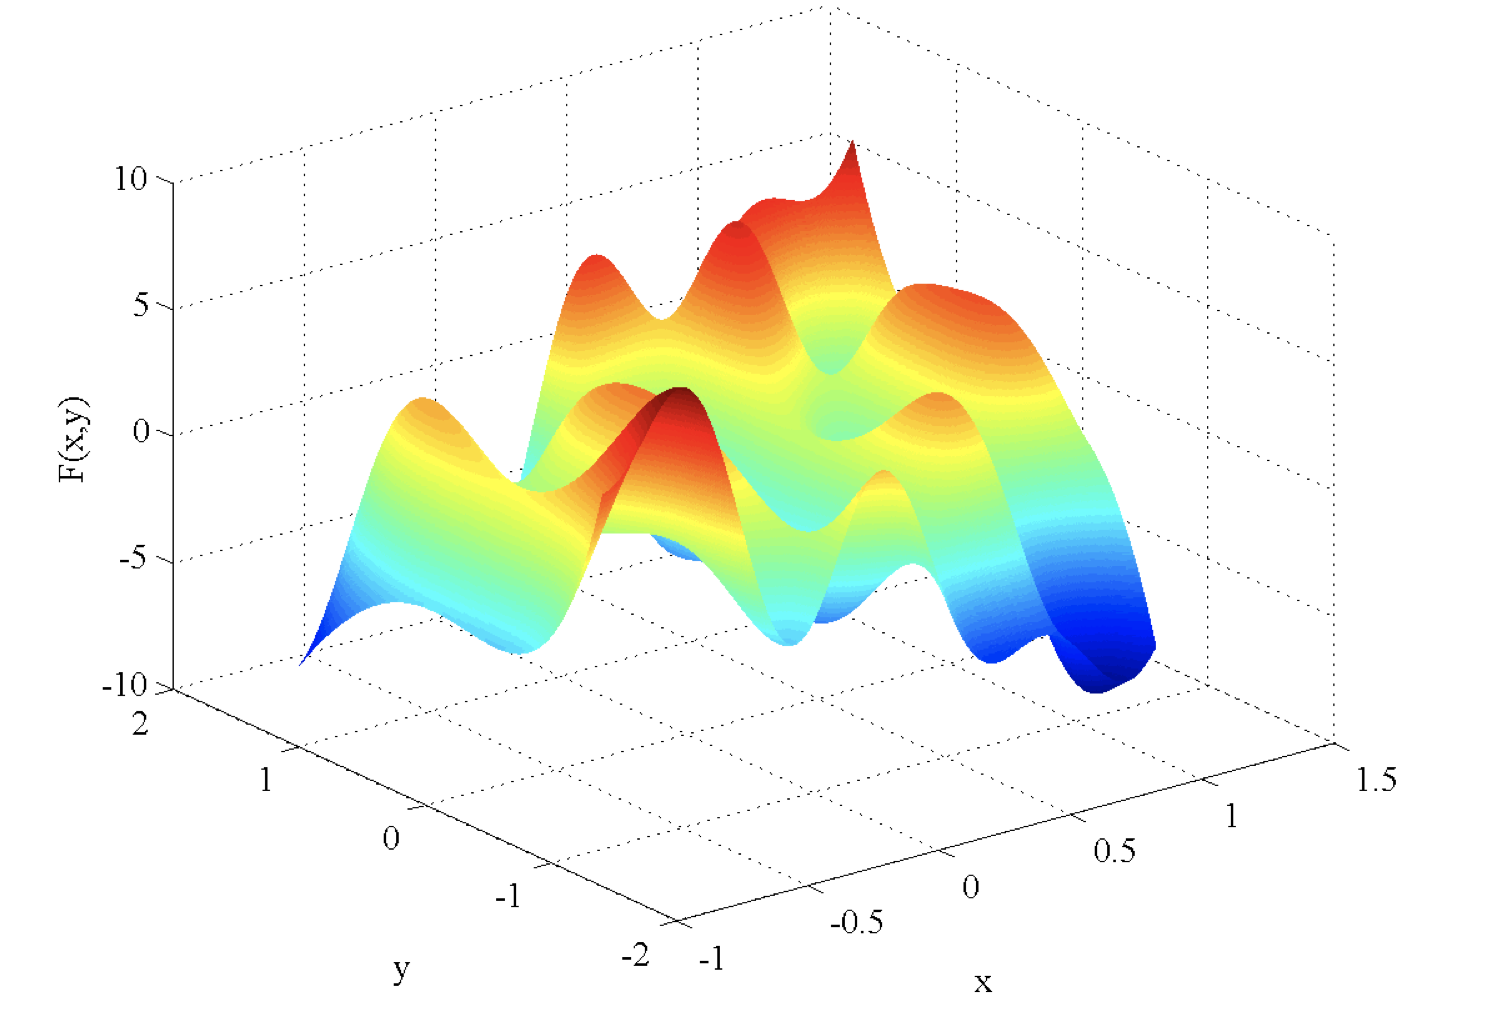
\includegraphics[width=0.9\textwidth]{assets/img/02_Grundlagen/ExampleSearchspace.png}
    }
    \caption{Beispielhafte Darstellung eines kontinuierlichen Such- oder Optimierungsraums einer Zielfunktion $f(x, y)$ mit zwei Variablen $x, y$. } 
    \label{img:example_searchspace}
    \source{\cite[S. 627]{kashtiban_solving_2016}}
\end{figure}

Abbildung \ref{img:example_searchspace} stellt einen kontinuierlichen Suchraum einer beliebigen Funktion $f(x, y)$ mit zwei Variablen dar. Das Ziel zur Lösung eines Optimierungsproblems besteht darin, die Definitionen der Variablen zu bestimmen, für welche die Costs (dt. Kosten) gemäß der Cost Function (dt. Kostenfunktion) am minimalsten bzw. maximalsten ist. In der Abbildung ist eine Vielzahl von lokalen Optima zu erkennen. Listing \ref{lst:localsearch} beschreibt einen \ac{LS}-Algorithmus, welcher anhand einer initialen Lösung (z. B. durch das Anwenden von Heuristiken generiert) über eine Anzahl an Iterationen oder einer Zeitvorgabe iterativ die nächstbeste Lösung innerhalb einer Nachbarschaft $N(s)$ auswählt. Das Problem hinter dieser Suchlogik besteht darin, dass dadurch ein lokales Optimum erreicht wird, welches nicht mehr über den Algorithmus verlassen werden kann.  \cite[vgl.][S. 3]{mills_survey_2004}

\begin{lstlisting}[caption={{Local Search (LS)}}, label=lst:localsearch, mathescape=truexinputencoding={utf8}, extendedchars=false, escapeinside=``]
Create an initial solution $s$ inside the search space;
while stopping criteria not satisfied do
    Select best solution $s' \in N(s)$;
    $s \leftarrow s'$; 
end
return the best solution;
\end{lstlisting}

Innerhalb eines hyperdimensionalen Lösungsraums, wie dies beim \ac{rcpsp} der Fall ist, kann die Anwendung von der naiven lokalen Suche abhängig vom Szenario zu unbefriedigenden Ergebnissen führen. Die Ergebnisse können mehr oder weniger stark vom globalen Optimum abweichen. \\

Als Teilbereich der künstlichen Intelligenzen stellen Metaheuristiken die Werkzeuge zur intelligenten Suche von Lösungen innerhalb von Such- und Optimierungsproblemen dar. Das Ziel von Metaheuristiken gegenüber der lokalen Suche liegt darin, dass lokale Optima vermieden oder verlassen werden können, um so das globale Optimum eines Lösungsraums zu finden. \cite[vgl.][S. 3]{mills_survey_2004} \\

Der Vorteil von Metaheuristiken gegenüber Heuristiken liegt darin, dass diese für alle Arten von diskreten Optimierungsproblemen generisch einsetzbar sind. Das Umgehen mit dem Phänomen der kombinatorischen Explosion innerhalb eines Optimierungsproblems, die Vermeidung der Nutzung von Gradientenberechnungen über die Zielfunktion, die Anlehnung an Naturwissenschaften orientierten Ansätzen, welche in der Physik, Biologie oder Ethologie vorzufinden sind, stellen weitere Vorteile und Merkmale von Metaheuristiken dar. Nachteile von Metaheuristiken sind jedoch die Bestimmung der Hyperparameter innerhalb der Algorithmen und die möglicherweise längere Berechnungsdauer. \cite[vgl.][S. 2 f.]{mills_survey_2004} \\

Dieser Abschnitt befasst sich mit der Einführung von populären Metaheuristiken für diskrete Optimierungsprobleme. Zuerst wird die Tabu Search im Abschnitt \ref{subsec:Grundlagen_TabuSearch} vorgestellt. Eine in der Metallurgie inspirierte Metaheuristik stellt Simulated Annealing (dt. simuliertes Abkühlen) dar, welche im Abschnitt \ref{subsec:Grundlagen_SimulatedAnnealing} eingeführt wird. Evolutionäre Algorithmen, konkret die genetischen Algorithmen, stellen eine aus der Biologie orientierte Metaheuristik dar. Diese werden im Abschnitt \ref{subsec:Grundlagen_EvolutionäreAlgorithmen} behandelt.


\subsection{Tabu Search} \label{subsec:Grundlagen_TabuSearch}

Die Tabu Search (zu dt. Tabu-Suche) wurde von Fred Glover im Jahre 1986 vorgeschlagen \cite[vgl.][S. 37]{gendreau_handbook_2019} und gilt als eine Erweiterung der \acf{LS}, welche bereits im übergeordneten Abschnitt eingeführt wurde. Der Vorteil der \acf{TS} gegenüber der \ac{LS} ist der Umgang mit lokalen Optima über das Nutzen einer Tabu-Liste. Hierbei werden Lösungen innerhalb einer Nachbarschaft ausgeschlossen, die sich bereits in der Tabu-Liste befinden. Die lokale Suche samt Einhaltung einer Tabu-Liste als Kurzzeitgedächtnis stellt die Basisversion der \ac{TS} dar. \cite[vgl.][S. 40]{gendreau_handbook_2019} \\

Beim Erreichen eines lokalen Optimums findet innerhalb der \ac{LS} in jeder Iteration ein repetitiver Wechsel zweier Lösungen statt. Durch diese Wechselschleife bis zur Terminierung des Algorithmus wird das lokale Optimum nicht mehr verlassen. \cite[vgl.][S. 40]{gendreau_handbook_2019} 

\begin{lstlisting}[caption={Tabu Search (Quelle: \cite[vgl.][S. 42 ff.]{gendreau_handbook_2019}}), label=lst:tabusearch, mathescape=truexinputencoding={utf8}, extendedchars=false, escapeinside=``]
Create an initial solution $s$ inside the search space;
Init tabu list $TL \leftarrow \emptyset$;
while stopping criteria not satisfied do
    Select best solution $s' \in N(s) \setminus TL$;
    $s \leftarrow s'$; 
    Add $s'$ to the tabu list $TL$;
    If tabu list $TL$ is full, remove oldest entry;
end
return the best solution;
\end{lstlisting}

Listing \ref{lst:tabusearch} beschreibt den Algorithmus der Tabu-Suche. Eine Tabu-Liste $TS$ stellt das Kurzzeitgedächtnis dar, welches nur eine feste Anzahl an Einträgen beinhalten kann und im initialen Zustand zunächst leer ist. Die Größe der Tabu-Liste $|TS]$ stellt ein Hyperparameter dar, welcher somit bei der Implementierung zu definieren ist. In jeder Iteration wird die ausgewählte Lösung, welche der besten Lösung einer Nachbarschaft entspricht, in die Tabu-Liste an erster Stelle hinzugefügt. Bestehende Einträge werden folglich um eine Stelle in der Liste weiterpropagiert. Einträge aus der Tabu-Liste dürfen nicht mehr aus einer Nachbarschaft $N(s)$ ausgewählt werden. Sofern die Tabu-Liste voll ist, wird das älteste Element entfernt und darf somit wieder ausgewählt werden. Durch das Ausschließen der Listeneinträge ist ein repetitiver Wechsel zweier Lösungen, wie es bei der \ac{LS} der Fall ist, je nach Größe der Tabu-Liste vermeidbar. Zudem wird der Suchraum um einen größeren Bereich erkundet und lokale Optima können verlassen werden. \cite[vgl.][S. 42 ff.]{gendreau_handbook_2019} \\

Sowohl in der lokalen Suche als auch in der Tabu-Suche ist eine Nachbarschaftsfunktion vorgesehen. Die Nachbarschaftsfunktion $N(s)$ stellt eine Submenge von Lösungen eines Suchraums dar. Diese beinhaltet Lösungen, welche von einer Ausgangslösung $s$ mit einem Move $m$ (dt. Schritt) erreichbar sind. Ein Move $m$ wird als eine charakterisierte Modifikation an einer Lösung bezeichnet. \cite[vgl.][S. 56]{siarry_metaheuristics_2016} \\

Beispielhaft visualisiert Abbildung \ref{img:example_neighbourhood} den Lösungsraum einschließlich der Nachbarschaftsbeziehungen von allen Permutationen von vier Elementen. Die Nachbarschaftsbeziehungen unterscheiden sich je nach Optimierungsproblem und müssen folglich für jedes Problem gesondert selektiert werden \cite[vgl.][S. 57 f.]{siarry_metaheuristics_2016}. Gemäß des Beispiels in der Abbildung wäre die Nachbarschaft für die Lösung 1234 über $N(1234) = \{ 1324, 1432, 2134 \}$ definiert, da nur ein Move notwendig ist, um diese Lösungen zu erreichen.  

\begin{figure}[H]
    \centering
    \noindent\makebox[\textwidth]{%
    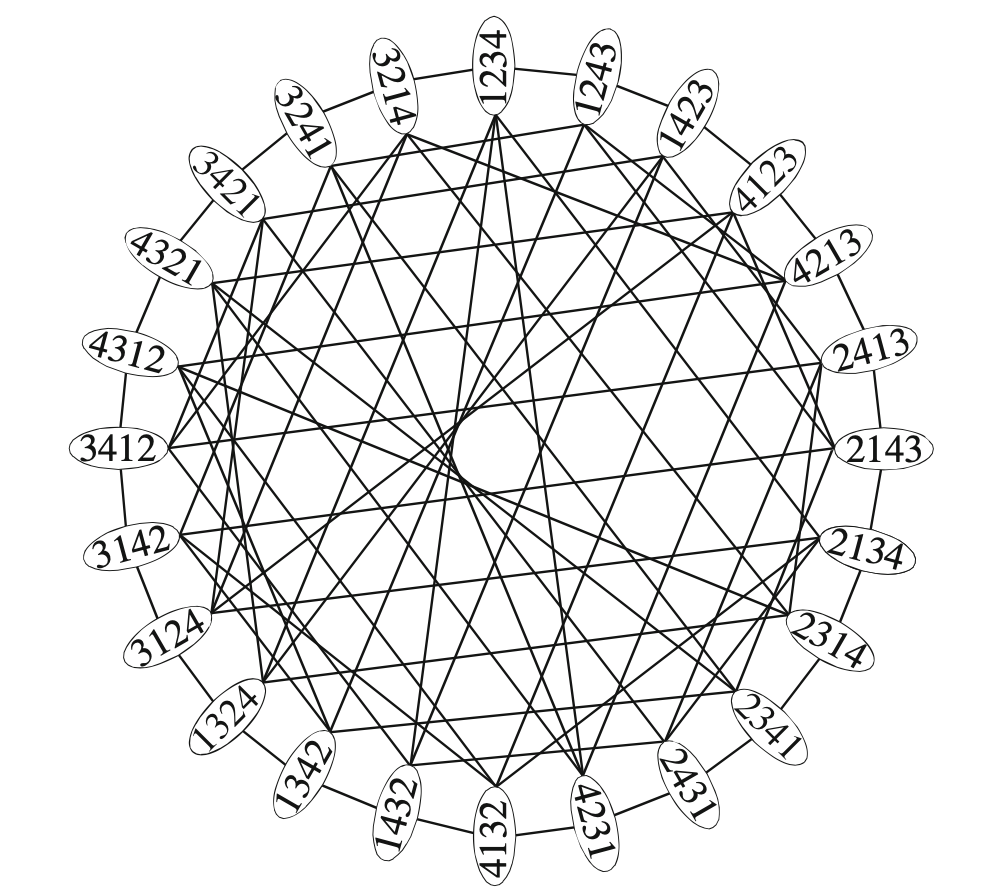
\includegraphics[width=0.74\textwidth]{assets/img/02_Grundlagen/Neighbourhood.png}
    }
    \caption{Nachbarschaftsbeziehungen einer Menge von Permutationen aus vier Elementen in Knotenform} 
    \label{img:example_neighbourhood}
    \source{\cite[][S. 57]{siarry_metaheuristics_2016} }
\end{figure}

Bei der Tabu-Suche stehen wie auch bei anderen Metaheuristiken, unterschiedliche Möglichkeiten zur Terminierung der Algorithmen zur Verfügung. Ein Algorithmus kann nach einer festen Anzahl an Iterationen oder CPU-Zeit beendet werden. Ein Algorithmus kann zudem auch nach einer bestimmten Anzahl an Iterationen, wo keine Verbesserung der Zielfunktion vorzufinden ist, terminiert werden. Eine weitere Möglichkeit ist, dass ein Algorithmus solange durchiteriert wird, bis ein definierter Schwellwert erreicht wurde. \cite[vgl.][S. 44]{gendreau_handbook_2019} 

\subsection{Simulated Annealing} \label{subsec:Grundlagen_SimulatedAnnealing}

Eine an der Physik, nämlich an der Metallurgie, orientierte Metaheuristik stellt \acf{SA} (dt. simuliertes Abkühlen) dar und wurde von den 3 IBM Wissenschaftlern Kirkpatrick, Gelatt und Vecchi im Jahre 1992 vorgeschlagen und im Jahr 1993 veröffentlicht. \cite[vgl.][S. 19]{siarry_metaheuristics_2016} \\

Für einen gegebenen Körper gilt es, nachdem dem Körper eine sehr hohe Temperatur zugeführt wurde, einen energetisch günstigen Zustand zu erreichen. Durch das Erhöhen der Temperatur zu einem sehr hohen Punkt wird die Struktur des Körpers zunächst geschmolzen. Der Körper befindet sich somit in einer flüssigen Phase, in welcher die Partikel des Körpers zufällig verteilt sind. Der Körper wird über das Abkühlen gemäß eines besonderen Temperaturschemas wieder in eine stabile Phase zurückgeführt und erreicht somit einen energetisch günstigen Zustand. Sowohl die initiale Temperatur als auch die Kühlungszeit müssen eine entsprechende Höhe aufweisen, da ansonsten ein metastabiler Zustand erreicht wird, in welcher die Energie nicht minimal ist. Der Prozess wird Härtung genannt, wenn die Temperaturabnahme nicht stetig ist und durch eine abrupte Abkühlung beeinflusst wird. Die Funktionsweisen und die Unterschiede zwischen dem Härtungs- und dem Abkühlungsprozess lassen sich über die Abbildung \ref{img:simulatedannealing_realworld} visualisieren. \cite[vgl.][S. 2 f.]{gendreau_handbook_2019} 

\begin{figure}[H]
    \centering
    \noindent\makebox[\textwidth]{%
    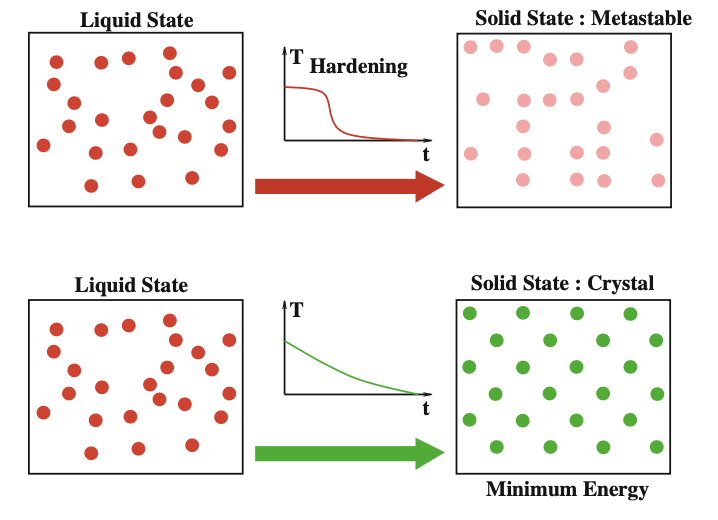
\includegraphics[width=0.48\textwidth]{assets/img/02_Grundlagen/SimulatedAnnealing_RealWorld.png}
    }
    \caption{Funktionsweise der Abkühlungs- und Härtungsprozesse} 
    \label{img:simulatedannealing_realworld}
    \source{\cite[][S. 3]{gendreau_handbook_2019} }
\end{figure}

Zwischen einem Optimierungsproblem und dem physikalischen System lassen sich Analogien ziehen. In der Physik wird die freie Energie betrachtet, bei dem Optimierungsproblem die Zielfunktion. Die Positionierung der Partikel stellt die Analogie zu den Parametern eines Problems dar. Das Ziel innerhalb eines physikalischen System liegt darin, dass ein energiearmer Zustand erreicht wird. Dies trifft ebenfalls bei Optimierungsproblemen zu, bei welchen Konfigurationen gesucht werden, welche als \glqq gut\grqq{} klassifiziert werden können oder im besten Fall am optimalsten sind. \cite[vgl.][S. 20]{siarry_metaheuristics_2016} 

\begin{lstlisting}[caption={Simulated Annealing (Quelle: \cite[vgl.][S. 714]{hosseinabadi_novel_2017}}), label=lst:simulatedannealing, mathescape=truexinputencoding={utf8}, extendedchars=false, escapeinside=``]
Create an initial solution $s$ inside the search space;
Select initial temperatur $T_0$;
Select rate of temperature decrease $\alpha \in [0.80, 0.99]$;
$T \leftarrow T_0$;  
while stopping criteria not satisfied do
    Select random solution $s' \in N(s)$;
    if f(s') < f(s)
        $s \leftarrow s'$;
    else
        $\Delta \leftarrow f(s') < f(s)$; 
        if random(0, 1) $< \exp(- \dfrac{\Delta}{T}$)
            $s \leftarrow s'$;
    $T \leftarrow T * \alpha$;
end
return the best solution;
\end{lstlisting}

Innerhalb des Algorithmus aus Listing \ref{lst:simulatedannealing} wird zunächst eine initiale Temperatur $T_0$ ausgewählt. Die Senkung anhand eines Temperaturschemas wird über eine Temperatursenkungsrate $\alpha \in [0.80, 0.99]$ realisiert. Wie auch bei der \ac{LS} wird eine initiale Lösung $s$ benötigt, welche zufällig oder über Heuristiken erzeugt werden können. Die initiale Lösung und Temperatur entsprechen dem flüssigen Zustand im Abkühlungsprozess. Nach jeder Iteration innerhalb des Algorithmus wird die Temperatur mit der Temperatursenkungsrate multipliziert $T \leftarrow T * \alpha$, was nach jeder Iteration zu einer Senkung der Temperatur führt. Um die Analogie zur Verfestigung zu realisieren, nutzt der Algorithmus die Nachbarschaftsfunktion, um so eine zufällige Lösung $s'$ auszuwählen. Über die Nutzung einer Akzeptanzfunktion gemäß Formel \ref{align:sa_acceptance} \cite[vgl.][S. 6]{gendreau_handbook_2019} und das Generieren einer zufälligen Zahl $r \in [0, 1]$ wird die Akzeptanz der Lösung $s'$ bestimmt. Sofern $r \leq P(s, s')$ gilt, wird die aktuelle Lösung überschrieben $s \leftarrow s'$. Das Annehmen von verschlechternden Lösungen im Algorithmus trägt maßgeblich zur Erkundung des Suchraums bei. Die Akzeptanz von schlechteren Lösungen sinkt über die Iterationen, da die ebenfalls sinkende Temperatur maßgebend zum Akzeptanzwert ist. Eine sinkende Temperatur impliziert, dass die Partikel innerhalb eines physikalischen Systems sich weniger stark bewegen. Gänzlich werden bei einer Temperatur $T \approx 0$ schlechtere Lösungen abgelehnt, was dazu führt, dass der Algorithmus lediglich als lokale Suche agiert. Es werden dann nur Lösungen angenommen, wenn die selektierte Lösung aus der Nachbarschaft besser als die aktuelle ist. \cite[vgl.][S. 5 f.]{gendreau_handbook_2019} \cite[vgl.][S. 21 f.]{siarry_metaheuristics_2016} 

\begin{align}
P(s, s') = \left\{\begin{array}{ll} 
        1 & \text{wenn $f(s') < f(s)$} \\
        e^{\Big(\dfrac{f(s) - f(s')}{T}\Big)} & \text{sonst} \\
     \end{array}\right. \label{align:sa_acceptance}
\end{align}

Wie bei der \ac{TS} stehen beim \ac{SA} unterschiedliche Stopkriterien zur Verfügung. Der Algorithmus von \cite[][S. 6 f.]{gendreau_handbook_2019} iteriert solange, bis die Temperatur bei $T \approx 0$ liegt. Der Algorithmus von \cite[][S. 714]{hosseinabadi_novel_2017} nutzt zusätzlich eine feste Anzahl an Iterationen, die durchlaufen werden müssen. Alternativ können die aus dem Abschnitt \ref{subsec:Grundlagen_TabuSearch} für die \ac{TS} vorgestellten Kriterien verwendet werden. Ein weitere Besonderheit stellt die Verwendung einer Boltzmann Konstante $k_B$ dar, welche zur Gewichtung der Temperatur in der Annahmefunktion beiträgt \cite[vgl.][S. 21]{siarry_metaheuristics_2016}. Durch die Verwendung einer Boltzmann Konstante $k_B$ lässt sich die Relevanz der Temperatur bei der Akzeptanzfunktion verändern.  

\input{pages/02_Grundlagen/023_EvolutionäreAlgorithmen}
\section{Stand der Forschung} \label{sec:StandForschung}
% Berücksichtigung weiterer Robustness Verfahren ("Eine Evaluierung weiterer Robustheitsfunktionen für das MRCPSP stehen noch aus. ")

% Weitere Problemerweiterungen
% Paper: http://archive.ceciis.foi.hr/app/public/conferences/1/papers2012/iis7.pdf

% Zusammenhang zwischen Metaheuristiken und (M)RCPSP


Der Einsatz von Metaheuristiken für das (M)\ac{rcpsp} stellt keineswegs einen unerforschter Bereich dar. Bereits 1998 verglichen \cite{kolisch_heuristic_1998} die Leistungen der Metaheuristiken für das Finden von optimalen Zeitplänen im Bezug auf die Projektdauer. Hierbei wurden unterschiedlich implementierte Metaheuristiken wie die \acl{TS}, \acl{SA} und \acl{GA} von Wissenschaftlern für das \ac{rcpsp} quantitativ verglichen \cite[vgl.][S. 17 f.]{kolisch_heuristic_1998}.\\

Für die Multi-Mode Problemerweiterung wurden ebenfalls bereits eine Vielzahl an Metaheuristiken entworfen. Allein für die genetischen Algorithmen existiert eine Vielzahl von wissenschaftlichen Veröffentlichungen, wie der im Jahre 2003 publizierte Artikel von \cite{alcaraz_solving_2003}. Weitere Artikel stellen beispielsweise die im Jahr 2013 veröffentlichte Arbeit von \cite{li_solving_2013} oder 2015 von \cite{sebt_efficient_2015} dar. Diese Arbeiten beziehen sich alle auf das \ac{mrcpsp}, aber unterscheiden sich unter anderem stark ihren Repräsentationsformen, Crossover-, Mutations- und Selektionsoperatoren oder die Wahl der Hyperparameter. Abseits von den genetischen Algorithmen wurde unter anderem 2001 von \cite{jozefowska_simulated_2001} ein Simulated Annealing-Algorithmus für das \ac{mrcpsp} implementiert. Innerhalb eines Papers zum reaktiven Scheduling wurde 2011 von \cite{deblaere_reactive_2011} ein Tabu Search-Algorithmus umgesetzt. \\

Das Thema der Unsicherheiten und der prädiktive Umgang wurde 2005 von \cite{al-fawzan_bi-objective_2005} in einem Artikel behandelt. In Kombination mit einer multi-objective Tabu Search gilt es die Projektdauer zu minimieren und zugleich die Robustheit zu maximieren. Durch die Maximierung der Robustheit können Pläne im Vornherein gefunden und die Projektverspätungen durch eine erhöhte Puffergröße minimiert werden \cite[vgl.][S. 177 f.]{al-fawzan_bi-objective_2005}. \\

Abseits der Maximierung der Summe aller Aktivitätspuffer existiert eine Vielzahl an Robustheitsfunktionen. 2013 wurden im Artikel von \cite{khemakhem_efficient_2013} bestehende und neue Robustheitsmessungen für das \ac{rcpsp} verglichen. \\

Die Verspätungen durch Unsicherheiten können zudem reaktiv gemindert werden. 2011 nutzte \cite{deblaere_reactive_2011} als reaktives Verfahren für das \ac{mrcpsp} unter anderem baumbasierte Suchtechniken, um so die Reschedule Costs bei den Unsicherheitszeitpunkten zu minimieren \cite[vgl.][S. 66]{deblaere_reactive_2011}. \\

2012 wurde in einer Erhebung von \cite{brcic_resource_2012} sowohl proaktive, prädiktive als auch für die reaktive Verfahren sowohl für das \ac{rcpsp} als auch die stochastische Version S\ac{rcpsp} aufgeführt. Im Fazit der Erhebung wurde anhand Daten verschiedener Publikationen hervorgehoben, dass im Bezug zum Basisproblem proaktive Verfahren besser für quantifizierbare Unsicherheiten und reaktive Verfahren geeigneter für weitaus größere Unsicherheiten sind. \\

Diese Masterarbeit baut auf den Ausblick von \cite[S. 405 f.]{brcic_resource_2012} auf und betrachtet Unsicherheiten für das \ac{mrcpsp}, was eine generalisierte Variante des \ac{rcpsp} darstellt. Die zitierte Erhebung baut auf quantitative Daten einzelner Publikationen auf, welche unterschiedliche Unsicherheitsszenarien und Verfahren zur Lösung des \ac{mrcpsp} aufweisen. Es gilt somit festzustellen, wie sich die Verfahren aus den pro-, prä- und reaktiven Methoden quantitativ auf eine gemeinsame Basis von Unsicherheitsszenarien und Metaheuristiken auswirken. Zudem kann evaluiert werden, wie sich die Leistung der unterschiedlichen Metaheuristiken nach Anwenden der Unsicherheitsszenarien auf die Projektdauer bei den einzelnen Verfahren auswirken. Die aufgeführten Themen liefern zum Zeitpunkt der Thesis noch Forschungsbedarf, was die Existenz der Forschungsfrage und dessen Unterfragen aus Abschnitt \ref{sec:Ziele} begründen soll. 
%  Ebenfalls im Ausblick von \cite[S. 405 f.]{brcic_resource_2012} vorzufinden gilt es noch die Robustheitsoptimierung innerhalb der reaktiven Verfahren zu evaluieren.

% Forschungslücke
% - Quantitativ mit gleichen Unsicherheitsszenarien / Solvervarianten, da dies in der Arbeit kritisiert wurde
% - MRCPSP anstelle von RCPSP
% - Impact von Metaheuristiken 


\chapter{Konzept des MRCPSP-Frameworks} \label{ch:Konzept}

Dieses Kapitel befasst sich mit der Konzeption eines MRCPSP-Frameworks, welches zur Beantwortung der Forschungsfrage und dessen Unterfragen maßgeblich ist. Hierfür wird im Abschnitt \ref{sec:Konzeptüberblick} zunächst ein Überblick der Anforderungen gegeben, welche zu implementieren sind. Basierend auf den Anforderungen werden im selben Abschnitt die Teilaspekte des Frameworks hergeleitet. Konzeptionsentscheidungen, wie die Auswahl der Verfahren für den Umgang von Unsicherheitsentscheidungen (Abschnitt \ref{sec:AuswahlVerfahrenUnsicherheiten}) und die Auswahl der Metaheuristiken (Abschnitt \ref{sec:AuswahlMetaheuristischenAlgorithmen}) werden ebenfalls im Kapitel behandelt. Um Vergleiche auf eine gemeinsame Datenbasis zu realisieren, befasst sich Abschnitt \ref{sec:Benchmarkdatensatz} mit der Auswahl des Benchmarkdatensatzes. Die Konzeption von Unsicherheitsszenarien wird im Abschnitt \ref{sec:Unsicherheitsszenarien} behandelt. 

% \section{Problemstellung} \label{sec:Problemstellung}

\input{pages/03_Konzept/02_Konzeptüberblick}
\section{Auswahl der Verfahren zur Lösung von Unsicherheiten} \label{sec:AuswahlVerfahrenUnsicherheiten}

Bereits im Abschnitt \ref{subsec:MRCPSP_Unsicherheiten} wurden Verfahren zur Lösung von Unsicherheiten vorgestellt. Aufgrund der zeitlichen Restriktionen dieser Arbeit werden jeweils ein konkretes Verfahren aus den Kategorien der pro-, prä-, und reaktiven Methoden verglichen. Ziel der Verfahren besteht darin, die verursachten Verspätungen der Unsicherheiten so gering wie möglich zu halten. Folgende Verfahren stehen repräsentativ für ihre jeweiligen Kategorien:

\begin{description}
\item[Proaktiv] Bei proaktiven Verfahren werden die Unsicherheiten ignoriert. Zeitpläne werden somit nur nach der minimalen Makespan $C_{max}$ selektiert. Dieses Verfahren dient im Rahmen der Masterarbeit als ein Referenzwert. Verfahren, die Unsicherheiten berücksichtigen, sollten bessere Ergebnisse als die proaktive Herangehensweise liefern. 

\item[Prädiktiv] Als prädiktive Herangehensweise wird neben der Minimierung der Makespan $C_{max}$ die Robustheit $\Omega$ von Zeitplänen maximiert. Es existieren für das \ac{rcpsp} eine Vielzahl an Robustheitsmessungsfunktionen (vgl. Abschnitt \ref{subsec:Praediktive_Methoden}). Innerhalb eines Experimentes werden unterschiedliche Robustheitsmessungen verglichen, um so aus den unterschiedlichen Robustheitsmessungsfunktion die bestmögliche Variante für den direkten Vergleich der anderen Verfahren auszuwählen.  

\item[Reaktiv] Bei den reaktiven Verfahren wird zum Zeitpunkt der Unsicherheit reagiert. Diese Arbeit befasst sich im Rahmen der reaktiven Verfahren mit der Reparatur von Zeitplänen zum Unsicherheitszeitpunkt. Die Kostenfunktion $\mathcal{C}$ wird über eine gesonderte Implementierung des Tabu-Search-Algorithmus minimiert, um so ähnliche Zeitpläne zum Basiszeitplan zu erhalten. In Anlehnung an die Arbeit von \cite{deblaere_exact_2008} werden die Inflexiblilitätsgewichte über eine Binomialverteilung und Moduswechselkosten über eine Gleichverteilung zufällig generiert, wobei die Dummy-Endaktivität mit einem Gewicht von $w_n = 10 * |E(\mathcal{B}(n, p))|$ versehen ist. Der Erwartungswert der Binomialverteilung wird über einen Koeffizienten multipliziert, um so Verspätungen durch Unsicherheitsszenarien stärker zu bestrafen.

\end{description}

\newpage

\section{Auswahl der metaheuristischen Algorithmen} \label{sec:AuswahlMetaheuristischenAlgorithmen}

Im Abschnitt \ref{sec:Metaheuristiken} wurden Metaheuristiken für Optimierungsprobleme im Generellen vorgestellt. Für das (M)\ac{rcpsp} wurde bereits eine Vielzahl an Metaheuristiken konzipiert und miteinander verglichen \cite[vgl. ][S. 16 ff.]{kolisch_heuristic_1998}. Wie im vorherigen Abschnitt \ref{sec:AuswahlVerfahrenUnsicherheiten} beschrieben, kann in dieser Arbeit aufgrund zeitlicher Restriktionen nur eine Auswahl an Metaheuristiken implementiert und verglichen werden. \\

Die implementierten Metaheuristken müssen in der Lage sein, mehreren Zielfunktionen herrzuwerden. Bei dem prädiktiven Verfahren soll neben der Minimierung der Makespan $C_{max}$ die Robustheit $\Omega$ maximiert werden. Viele Multi-Objective Metaheuristiken nutzen daher Pareto-Prinzipien, um optimale Fronten zwischen mehreren Zielfunktionen zu definieren. Abbildung \ref{img:paretofront} zeigt eine beispielhafte Pareto-Front zweier Zielfunktionen auf. Während es bspw. $f_1$ zu maximieren gilt, soll $f_2$ minimiert werden. Dreiecke und Kreuze innerhalb der Grafik stellen schlechtere Kompromisse zweier Funktionen dar, da diese von anderen Lösungen, nämlich den Kreisen dominiert werden. \cite[vgl.][S. 285 ff.]{talbi_multi-objective_2012} \\

Im Rahmen der Arbeit werden die Zielfunktionen der Metaheuristiken strikt priorisiert. Die Makespan $C_{max}$ gilt als die primäre Zielfunktion, welches bei einem direkten Vergleich von mehreren Lösungen zunächst die bessere Lösung gemäß der minimalen Makespan selektiert. Die sekundäre Zielfunktion, welche die Robustheit $\Omega$ eines Plans darstellt kommt nur in Betracht, wenn mehrere Lösungen mit identischer Makespan verglichen werden. Hierbei wird die Lösung ausgewählt, welche die maximale Robustheit aufweist. 

\begin{figure}[H]
    \centering
    \noindent\makebox[\textwidth]{%
    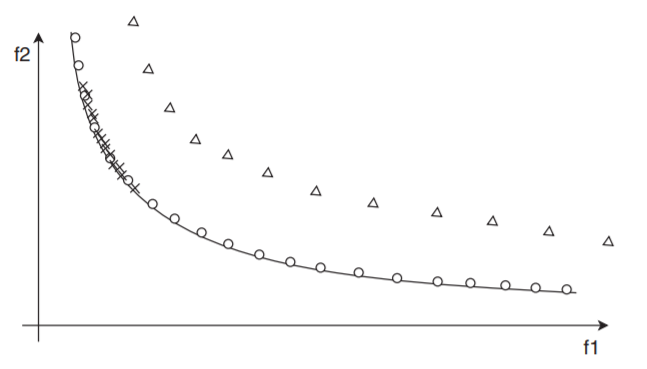
\includegraphics[width=0.75\textwidth]{assets/img/03_Konzept/Pareto.png}
    }
    \caption{Beispiel einer Pareto-Front zweier Zielfunktionen $f_1$ und $f_2$} 
    \label{img:paretofront}
    \source{\cite[vgl.][S. 286]{talbi_multi-objective_2012}}
\end{figure}

Die ausgewählten Metaheuristken entsprechen zum Zeitpunkt der Thesis den State-of-the-Art Lösungsverfahren für das \ac{mrcpsp}. Es werden die im Kapitel \ref{sec:Metaheuristiken} vorgestellten Metaheuristiken, angelehnt an den bestehenden Publikationen für das (M)\ac{rcpsp} gemäß der Problemstellung implementiert und verglichen. Des Weiteren werden die Metaheuristiken mit einem Random Solver und dem Hill Climbing-Algorithmus verglichen, welcher der naive lokale Suche entspricht:

\begin{description}
\item[Random Solver] Der Random Solver entspricht einer naiven Variante und erstellt ohne Heuristiken über das \ac{ssgs} zufällige Aktivitäts- und Modilisten. Der Random Solver dient für die Evaluation als eine Referenz, um die Ergebnisse der Metaheuriken besser vergleichen und interpretieren zu können. 

\item[Hill Climbing / \acf{LS}] Der generische \ac{LS}-Algorithmus gilt als eine weitere Referenz zwischen dem Random Solver und den Metaheuristiken. Iterativ wird über die Nachbarschaftsfunktion einer bestehenden Lösung die nächstbeste ausgewählt (vgl. Kapitel \ref{sec:Metaheuristiken}).  

\item[\acf{TS}] Die \ac{TS} wurde in unterschiedlichen Versionen bereits 1999 von \cite[S. 9]{kolisch_heuristic_1998} für das \ac{rcpsp} aufgegriffen. Eine Variante verwendet als Nachbarschaft einer Lösung eine Menge von ausgehenden Lösungen mit einzelnen Aktivitätstauschen \cite[vgl.][S. 5]{thomas_tabu_1998}. 

\item[\acf{SA}] Abermals wurde 1999 von \cite[S. 9]{kolisch_heuristic_1998} für das \ac{rcpsp} die Simulated Annealing-Metaheuristik aufgegriffen. Hierbei wurde, wie bei der \ac{TS}, die Nachbarschaft aus einzelnen Aktivitätstauschen realisiert. 

\item[\acf{GA}] Ebenfalls wurden in der Publikation von \cite[S. 9]{kolisch_heuristic_1998} für das \ac{rcpsp} eine Vielzahl an genetischen Algorithmen verglichen. Bei den Crossover Operatoren steht eine Vielzahl zur Verfügung: Darunter der One-Point Crossover, die Erweiterung, der Two-Point Crossover und die im Abschnitt \ref{subsec:Grundlagen_EvolutionäreAlgorithmen} bereits vorgestellte Uniform Crossover Operation \cite[vgl.][S. 4 f.]{hartmann_competitive_1998}. 

Als Mutation Operator können austauschbare Aktivitäten innerhalb einer Aktivitätsliste mit einer gewissen Wahrscheinlichkeit $p_{mutation}$ miteinander gewechselt werden. \cite[vgl.][S. 5]{hartmann_competitive_1998} 

Für das \ac{mrcpsp} können sowohl der Two-Point Crossover als auch der Mutation Operator genutzt werden \cite[vgl. ][S. 10 ff.]{rezaeian_using_2015}. Innerhalb dieser Thesis werden beide Operationen zur Realisierung des genetischen Algorithmus verwendet und im Abschnitt \ref{subsec:MetaheuristischeAlgorithmen_EvolutionaereAlgorithmen} erläutert.
\end{description}

Algorithmen, wie die \ac{LS}, \ac{TS} und \ac{SA} sehen alle eine Nachbarschaftsfunktion $N(s)$ vor. Diese wird innerhalb der Arbeit für alle Verfahren gleichermaßen implementiert. Aufgrund der möglichen hohen Anzahl an Kombinationen innerhalb einer Nachbarschaft, soll nur eine Teilmenge $\tilde{N}(s) \subset N(s)$ betrachtet werden. Dies geht aus der Publikation von \cite[S. 5]{thomas_tabu_1998} hervor. \\

Eine Publikation für das Lösen des \ac{mrcpsp} mithilfe von Simulated Annealing beschreibt drei Möglichkeiten zur Bildung einer Nachbarschaftsfunktion. Aktivitäten können innerhalb der Aktivitätsliste samt deren Modi verschoben werden. Zudem existiert die Möglichkeit, dass eine Aktivität zufällig selektiert wird und der zugehörige Modus auf einen anderen Modus geändert werden kann. Die dritte Variante stellt die Kombination der beiden vorherigen Varianten dar, welche in dieser Arbeit als Nachbarschaftsfunktion aufgegriffen wird. \cite[vgl.][S. 145]{jozefowska_simulated_2001}
\section{Benchmarkdatensatz} \label{sec:Benchmarkdatensatz}

Die zu implementierenden Metaheuristiken und proaktiven, prädiktiven und reaktiven Verfahren gilt es auf eine gemeinsame Datenbasis für das \ac{mrcpsp} zu validieren. Unzählige wissenschaftliche Arbeiten, wie die von \cite{rezaeian_using_2015}, \cite{jozefowska_simulated_2001} oder \cite{al-fawzan_bi-objective_2005} nutzen zur Evaluierung ihrer Ergebnisse für das \ac{mrcpsp} die PSPLIB von \cite{kolisch_psplib_1997}. Dort enthalten sind Instanzsets, welche neben unterschiedlich generierten Projektplänen auch die Informationen zu den minimalen Projektdauern beinhalten. 

\begin{table}[H]
\centering
\begin{tabular}{r|ccccc}
& m1  & m2  & n0  & n1  & j20 \\ \hline
Instanzen & 640 & 481 & 470 & 637 & 554 \\ \hline
Aktivitäten & 16  & 16  & 10  & 16  & 20  \\
Modi & 1   & 2   & 3   & 3   & 3   \\ \hline
Erneuerbare Ressourcenarten & 2   & 2   & 2   & 2   & 2   \\
Nicht erneuerbare Ressourcenarten & 2   & 2   & 0   & 1   & 2  
\end{tabular}

\caption{Metadaten zu den verwendeten Instanzsets der PSPLIB \cite{kolisch_psplib_1997}}
\label{tab:instanzsets}
\source{Eigene Darstellung}
\end{table}

Tabelle \ref{tab:instanzsets} repräsentiert fünf Instanzsets der PSPLIB von \cite{kolisch_psplib_1997}. Im Rahmen der Evaluierung werden diese verwendet, um die Metaheuristiken miteinander vergleichen zu können. Durch die unterschiedlichen Anzahlen von Aktivitäten, Modi und (nicht) erneuerbaren Ressourcenarten werden die Metaheuristiken mit andersartigen komplexen Gegebenheiten evaluiert. Die PSPLIB beinhaltet zudem das Instanzset j30.mm mit 30 Aktivitäten, in welcher die angegebenen minimalsten Projektdauern zum Zeitpunkt der Masterarbeit nur heuristisch sind, da globale Optima durch die immense Menge an Permutationen nicht bestimmt werden können.\\

Eine konkrete Instanz n01\_2.mm der PSPLIB vom Benchmarkset n0 kann aus Listing \ref{lst:psplib_n0_example} entnommen werden. Einzelne Sektionen zur Beschreibung des Projektplans werden über Sternchen- und Minuszeichen voneinander getrennt. Die ersten drei Sektionen geben Metainformationen, wie die Anzahl der Aktivitäten, Ressourcenarten, maximale Dauer über Horizon, und Daten zur Generierung der Instanz an. Der vierte Bereich zeigt zum einen die Abhängigkeiten der Aktivitäten und zum anderen die Anzahl der möglichen Modi für eine Aktivität auf. Die Modi werden in dem fünften Bereich mit einer Ausführdauer und den Ressourcenanforderungen definiert. Im sechsten und letzten Bereich der Datei werden die für das Projekt verfügbaren Ressourcen aufgeführt. 

\begin{lstlisting}[caption={Instanz n01\_2.mm der PSPLIB n0 (Quelle:  \cite{kolisch_psplib_1997})}, label=lst:psplib_n0_example, basicstyle=\scriptsize, breaklines=true,breakatwhitespace=true, columns=flexible]
************************************************************************
file with basedata            : me1_.bas
initial value random generator: 466396357
************************************************************************
projects                      :  1
jobs (incl. supersource/sink ):  12
horizon                       :  65
RESOURCES
  - renewable                 :  2   R
  - nonrenewable              :  0   N
  - doubly constrained        :  0   D
************************************************************************
PROJECT INFORMATION:
pronr.  #jobs rel.date duedate tardcost  MPM-Time
    1     10      0        8        6        8
************************************************************************
PRECEDENCE RELATIONS:
jobnr.    #modes  #successors   successors
   1        1          3           2   3   4
   2        3          3           5   7   9
   3        3          2           8   9
   4        3          3           5   6   7
   5        3          2          10  11
   6        3          2           8   9
   7        3          2          10  11
   8        3          2          10  11
   9        3          1          12
  10        3          1          12
  11        3          1          12
  12        1          0        
************************************************************************
REQUESTS/DURATIONS:
jobnr. mode duration  R 1  R 2
----------------------------------------
  1      1     0       0    0
  2      1     1       0   10
         2     6       6    0
         3     9       0    8
  3      1     3       4    0
         2     5       0    7
         3     7       0    4
  4      1     1       7    0
         2     5       0   10
         3     8       5    0
  5      1     1       0    5
         2     2       0    4
         3     6       2    0
  6      1     2       0    3
         2     3       8    0
         3     6       7    0
  7      1     6       6    0
         2     8       4    0
         3     9       3    0
  8      1     1      10    0
         2     2       8    0
         3     3       0    6
  9      1     1       7    0
         2     4       6    0
         3     4       0    6
 10      1     1       6    0
         2     1       0    7
         3     3       0    6
 11      1     1       0    3
         2     8       4    0
         3    10       3    0
 12      1     0       0    0
************************************************************************
RESOURCEAVAILABILITIES:
  R 1  R 2
    7    7
************************************************************************
\end{lstlisting}

In Abbildung \ref{img:psplib_n0_example} lässt sich der Projektplan für die Instanz n01\_2.mm grafisch visualisieren. Diese Darstellungsart ist angelehnt an die aus Abbildung \ref{img:example_mrcpsp}.

\begin{figure}[H]
    \centering
    \noindent\makebox[\textwidth]{%
    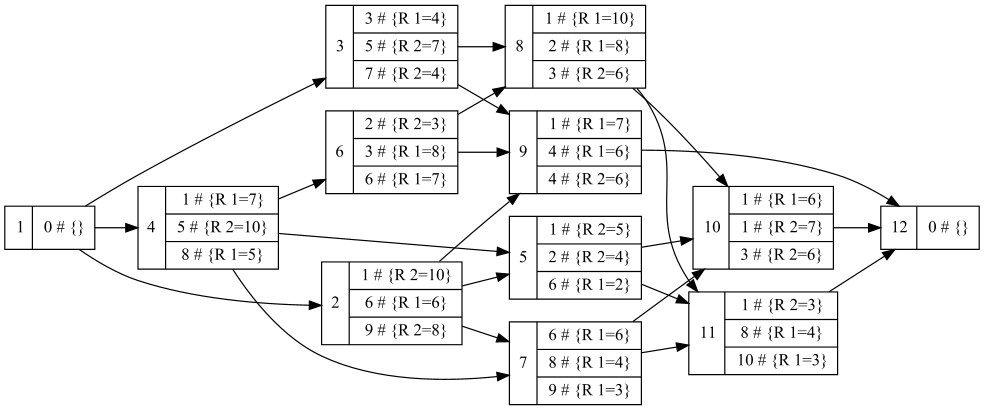
\includegraphics[width=\textwidth]{assets/img/03_Konzept/n01_2.png}
    }
    \caption{Visualisierung des Projektplans der Instanz n01\_2.mm der PSPLIB n0} 
    \label{img:psplib_n0_example}
    \source{Eigene Darstellung}
\end{figure}
\section{Unsicherheitsszenarien} \label{sec:Unsicherheitsszenarien}

Unsicherheiten, wie Aktivitäts- und Ressourcenstörungen müssen zunächst konzipiert und anschließend implementiert werden. Hierfür gilt es die Unsicherheiten in dem existierenden Benchmarkdatensatz aus Abschnitt \ref{sec:Benchmarkdatensatz} zu integrieren. In dieser Masterthesis werden die Aktivitätsstörungen als einzige Unsicherheitsart analysiert. \\

Um Unsicherheitsszenarien zu erzeugen, stehen unterschiedliche Arten für die Umsetzung zur Verfügung. \cite{khemakhem_efficient_2013} verwendet für den Vergleich von Robustheitsmessungen ein Störungsschema mit $\Delta_j = 0.20 \cdot d_j$ \cite[vgl. ][S. 260]{khemakhem_efficient_2013}. Folglich verspätet sich jede Aktivität um 20\%. \\

Durch eine fixe Verspätung über $\Delta_j = 0.2 \cdot d_j$ wäre somit jede Aktivität verspätet. Bei dem reaktiven Ansatz, wird zu einem Verspätungszeitpunkt ein neuer Zeitplan generiert. Dies führt dazu, dass nach jeder Aktivität ein neuer Zeitplan generiert werden muss. Bei einer hohen Anzahl an Aktivitäten kann diese Art von Störungsschema zeitaufwendig sein, da ohnehin das Erzeugen von neuen Zeitplänen bei den reaktiven Methoden sich als zeitintensiv herausgestellt hat (vgl. Abschnitt \ref{subsec:Reaktive_Methoden}). Zudem ist die Annahme, dass jede Aktivität sich um einen konstanten Faktor 20\% verspätet nicht zwingend realitätsnah. \\

Im Bezug auf die Aktivitätsstörungen nutzt \cite{deblaere_reactive_2011} die stetige Gleichverteilung, welche eine zufällige Verspätung zwischen $[1, d_j]$ auswählt \cite[vgl.][S. 72]{deblaere_reactive_2011}. Somit entspricht das Unsicherheitsszenario gemäß \cite{deblaere_reactive_2011} bei $\Delta_j = \mathcal{U}(1, d_j)$. \\

Im Rahmen dieser Masterarbeit sollen Verspätungen ebenfalls gemäß einer Verteilungsfunktion erzeugt werden. Dadurch, dass die Dauer $d_{j,m} \in \mathbb{N}$ einer natürlichen Zahl entspricht, sind diskrete Verteilungsfunktionen erforderlich. Die Binomialverteilung $\mathcal{B}(n, p)$ stellt das diskrete Pardon der Normalverteilung $\mathcal{N}(\mu, \sigma)$ dar, welche sich durch die Parametrisierung über die Versuchsanzahl $n$ und dem Wahrscheinlichkeitswert eines Vorkommens $p$ für das Generieren von Unsicherheitsszenarien eignet. Die Neigung einer Binomialfunktion wird über $p$ bestimmt. Bei $p > 0.5$ ist die Verteilung linksschief, bei $p < 0.5$ rechtsschief, ansonsten mit $p = 0.5$ symmetrisch. \\

Die Parametrisierung der Binomialverteilung $\mathcal{B}(n, p)$ erfolgt über das Berücksich-tigen von Definitionen von Annahmen. Die erste Annahme ist, dass eine Aktivität sich um maximal zwei Zeiteinheiten verspäten darf. Folglich wird $n \in \mathbb{N}$ mit zwei definiert, da neben den zwei Verspätungsfällen auch der Fall von keiner Verspätung über das nullte Element in der Verteilung abgedeckt wird. Zudem wird angenommen, dass ein Großteil der Aktivitäten pünktlich, ein kleinerer Teil mit einer Zeiteinheit und ein noch kleinerer Teil mit zwei Zeiteinheiten Verspätung abgeschlossen werden sollen. Da somit für den Parameter $p \in \mathbb{R}$ unzählige Möglichkeiten zur Verfügung stehen und zudem auch für die Intensität der Unsicherheiten ausschlaggebend ist, werden unterschiedliche Werte für $p$ zur Evaluierung verwendet, welche in Tabelle \ref{tab:binomial_uncertainty} aufgeführt sind. 

\begin{table}[H]
\centering
\begin{tabular}{r|ccc}
     & $p(\mathcal{B}(2, p) = 0)$ & $p(\mathcal{B}(2, p) = 1) $ & $p(\mathcal{B}(2, p) = 2)$ \\ \hline
p = 0\%  & 100\% & 0\% & 0\% \\
p = 5\%  & 90.25\% & 9.5\% & 0.25\%  \\
p = 10\% & 81\% & 18\% & 1\%  \\
p = 20\% & 64\% & 32\% & 4\% 
\end{tabular}
\caption{Wahrscheinlichkeitswerte für Aktivitätsstörungen gemäß der Binomialfunktion $\mathcal{B}(3, p)$}
\source{Eigene Darstellung}
\label{tab:binomial_uncertainty}
\end{table}

Durch das Erzeugen von Unsicherheitsszenarien für Aktivitätsstörungen über die Binomialfunktion $\Delta_j = \mathcal{B}(n, p)$ ist der Zufall ausschlaggebend. Insbesondere bei der Evaluierung der pro-/prä-/reaktiven  Verfahren sollten mehrere Unsicherheitsszenarien für einen zu betrachtenden Zeitplan $S$ durchlaufen werden. Erst durch das Durchlaufen unterschiedlicher Unsicherheitsszenarien können Aussagen über die tatsächlichen Leistungen der Verfahren gemacht werden. Dieses Problem ist bei dem deterministischen Ansatz über $\Delta_j = 0.2 \cdot d_j$ nicht vorzufinden, da im Vornherein alle Aktivitäten die gleiche Verspätung aufweisen. Zunächst ist die Berechnung mehrerer unterschiedlicher Experimente pro Zeitplan $S$ fraglos zeitaufwendiger, können aber heutzutage in der CPU bei entsprechender Anzahl der Kerne parallel ausgeführt werden.

% \[
% \mathcal{B}(n, p) = \binom{n}{k} % \cdot p^k \cdot (1 - p)^{n-k}
% \]

\chapter{Implementierung des MRCPSP-Frameworks} \label{ch:Implementierung}
In diesem Kapitel wird die Implementierung des \ac{mrcpsp}-Frameworks einschließlich der entwickelten Metaheuristiken vorgestellt. Zunächst gilt es die Struktur des Frameworks im Abschnitt \ref{sec:Strukturbeschreibung} basierend auf einem UML-Klassendiagramm aufzuzeigen. Das Thema der Zeitplanerstellung, Heuristiken und die Visualisierung wird im Folgeabschnitt behandelt. Abschnitt \ref{sec:Loesungsansaetze} stellt die unterschiedlich implementierten Lösungsansätze und Metaheuristiken vor. Der Aufbau von Experimenten, wie beispielsweise der Vergleich von den Lösungsansätzen oder die Handhabung von Unsicherheitsszenarien gilt es im Abschnitt \ref{sec:Experimente} zu vertiefen. % Zuletzt wird die Umsetzung von Visualisierungen im Abschnitt \ref{sec:Visualisierung} behandelt. 

\section{Strukturbeschreibung} \label{sec:Strukturbeschreibung}

Wie bereits im Abschnitt \ref{sec:Konzeptüberblick} erläutert wird für die Entwicklung des MRCPSP Framework die objektorientierte Programmiersprache Java einschließlich des Spring genutzt. Über die objektorientierte Programmierung können Teilaspekte der Anwendung über Klassen voneinander getrennt werden. Packages können zudem eingesetzt, um Aspekte voneinander zu trennen, um so den Code übersichtlicher zu halten. Innerhalb des MRCPSP Frameworks sind die Packages nach Kategorien angelegt. Folgende Paketstruktur ist mit entsprechenden Funktionen in der Umsetzung vorgesehen:

\begin{description}
\item[Rootpackage] \lstinline|de.uol.sao.rcpsp_framework| beinhaltet die Mainklasse und somit den Einstiegspunkt der Anwendung. Durch die Verwendung vom Spring Framework werden weitere Einstiegspunkte in der Anwendung über die Komponenten/Services Annotation festgelegt. 
\item[exception] Eigene Exceptions die innerhalb der Anwendung auftreten sind in diesem Package enthalten.
\item[experiment] Einzelne zu untersuchende Aspekte werden über Experimente geregelt.  
\item[heuristic] Klassen zur Generierung von Aktivitäts- und Moduslisten anhand bestimmter Prioritäts- und Modusregeln. 
\item[metric] Unterschiedliche Funktionen für Zeitplan-Metriken, um bestimmte Informationen, wie die Projektdauer oder Robustheit zu berechnen. 
\item[function] Zielfunktionen, die entweder für einen direkten Vergleich zweier Zeitpläne oder für die Fitness-Berechnung eines einzelnen Plans eingesetzt werden. 
\item[representation] Unterschiedliche Representationsformen von Aktivitäts- und Modusselektionen für Zeitpläne die innerhalb des \ac{mrcpsp} Frameworks verwendet werden können.
\item[scheduling] Klassen zum Erstellen von Zeitplänen und deren Informationen. 
\item[service] Mit \lstinline{@Service} annotierte Klassen, welche in der kompletten Anwendung an unterschiedlichen Stellen verwendet werden. 
\item[solver] Beliebige Lösungsverfahren u. a. Metaheuristiken, die in der Anwendung verwendet werden.
\item[helper] Hilfsklassen und deren Methoden, die über die komplette Anwendung genutzt werden und sich nicht in anderen Packages klassifizieren lassen. 

\end{description}

\begin{figure}
    \centering
    \noindent\makebox[\textwidth]{%
    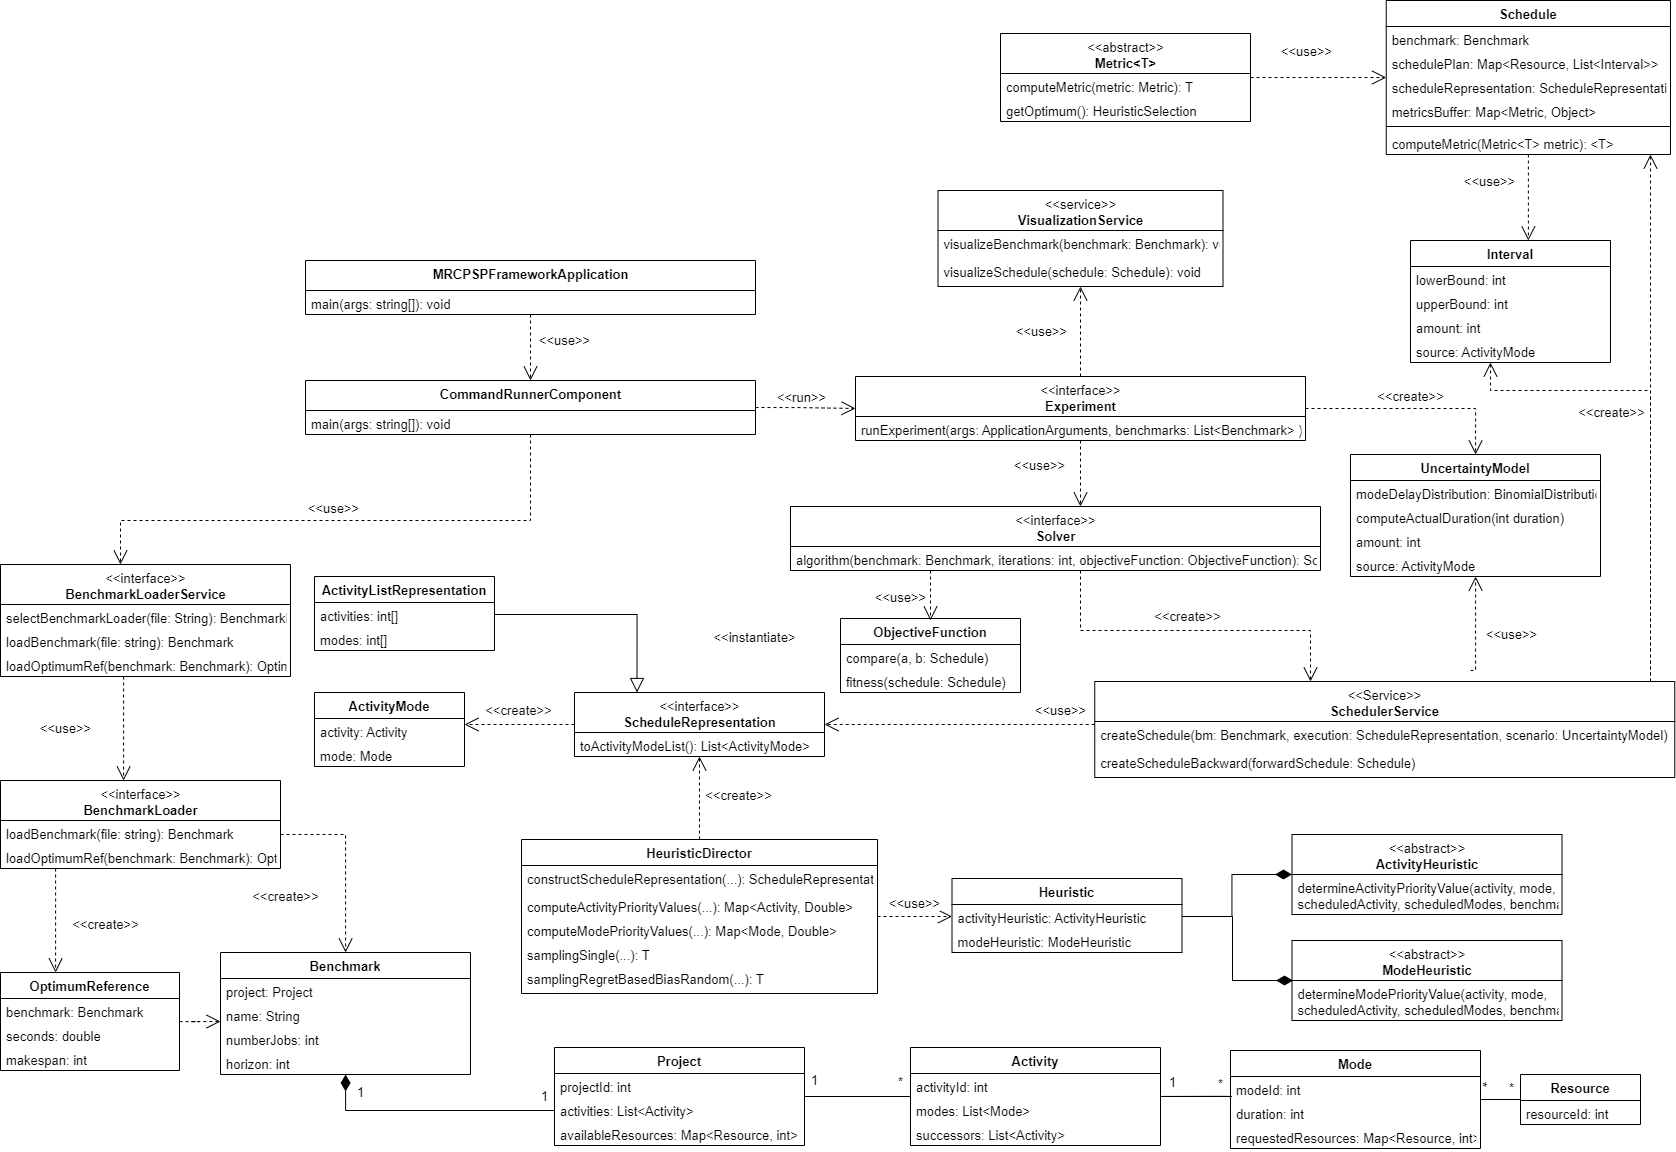
\includegraphics[angle=90,height=0.90\textheight]{assets/img/04_Umsetzung/Klassendiagramm_Minimized.drawio.png}
    }
    \caption{Zusammengefasstes UML-Klassendiagramm des MRCPSP-Framework} 
    \label{img:mrcpsp_framework_klassendiagramm}
    \source{Eigene Darstellung}
\end{figure}

Durch die Implementierung entstand das zusammengefasste UML-Klassendia-gramm aus Abbildung \ref{img:mrcpsp_framework_klassendiagramm}, welches aufgrund der Komplexität keine Generalisierungen von abstrakten Klassen und Interfaces berücksichtigt. Im Verlauf des Kapitels werden einzelne UML-Klassendiagramme zur Erläuterung der Umsetzung eingesetzt und erläutert, welche diese Generalisierungen aufführt. 

\newpage
\section{Zeitplanerstellung und Heuristiken} \label{sec:Heuristiken}

Um Zeitpläne für das \ac{mrcpsp} zu erstellen, gilt es die zugehörigen Constraints aus Abschnitt \ref{sec:MRCPSP} einzuhalten. Hierfür ist im Konzeptüberblick die Komponente \lstinline|Scheduler| vorgesehen. Des Weiteren müssen Lösungsansätze und Verfahren zur Lösung von Unsicherheiten auf eine gemeinsame Datenbasis verglichen werden, um für diese Zeitpläne erstellen zu können. Hierfür sind \lstinline|Benchmark Loader| und \lstinline|Benchmark Instance Sets| aus dem Abschnitt \ref{sec:Konzeptüberblick} vorgesehen. 

\subsection{Benchmarkinstanzen}

Zum Laden der Projektinstanzen von der PSPLIB ist ein \lstinline|BenchmarkLoaderService| implementiert, welcher anhand der Datenendung einen passenden Loader selektiert. Im Falle der PSPLIB für die Multi-Mode Projekterweiterung wird die Datenendung \lstinline|.mm| verwendet \cite[vgl.][S. 213 f.]{kolisch_psplib_1997}. Der vorgesehene \lstinline|BenchmarkPSPLIBMultiModeLoader| lädt aus der PSPLIB die vorgesehenen Struktur das Projekt einschließlich Metadaten, Aktivitäten, Aktivitätsbeziehungen, Modi und die Ressourcenanforderungen aus und überträgt diese innerhalb der im MRCPSP Framework vorgesehenen \acp{POJO}. Die einzelnen \acp{POJO} orientieren sich hierbei an den Subjekten und deren Beziehungen von der \ac{mrcpsp}-Problembeschreibung aus Abschnitt \ref{subsec:MRCPSP_MM}. Abbildung \ref{img:mrcpsp_framework_benchmarkloader} zeigt die Klassen des Benchmark Loaders und die der \acp{POJO} in einem UML-Klassendiagramm auf.

\subsection{Zeitplanerstellung}

Für die Erstellungen von \ac{mrcpsp}-Zeitplänen können unterschiedliche Repräsen-tationsformen verwendet werden. Neben den Aktivitäts- und Moduslisten existiert die Random Key Representation, welche in den Publikationen von \cite{sebt_efficient_2015} und \cite{kolisch_heuristic_1998} verwendet wird. Diese Arbeit beschränkt sich jedoch nur auf die Aktivitäts- und Moduslisten, welche in den Abschnitten \ref{subsec:SGS_Aktivitaeten} und \ref{subsec:SGS_Modi} eingeführt wurden. Hierfür ist eine Klasse \lstinline|ActivityListRepresentation| vorgesehen, die von der Klasse \lstinline|ScheduleRepresentation| erbt und zwei Felder für die Aktivitäten und für die Modi vorsieht. Diese Repräsentationsform wird von den (Meta-)Heuristiken zur Erstellung von Schedules genutzt. Abbildung \ref{img:mrcpsp_framework_schedulerheuristiken} stellt das UML-Klassendiagramm für die Realisierung der Repräsentationsform, aber auch der Zeitplanerstellung und Heuristiken dar. \\

Der \lstinline|SchedulerService| erzeugt mit der Methode \lstinline|createSchedule(...)| Zeitpläne anhand von Aktivitäten- und Modirepräsentationen $I = (\lambda, \mu)$ gemäß des \ac{ssgs}. Hierbei werden die Ressourcenbelegungen über Intervalle (\lstinline|Interval|) festgehalten. Listing \ref{lst:scheduler_forward} zeigt den Algorithmus für das sequenzielle Abarbeiten der Aktivitäten und den zugehörigen Modi (\lstinline|ActivityMode|) auf. Für jeden \lstinline|ActivityMode| wird ein identischer Intervall auf alle zu verwendenden erneuerbaren Ressourcen erzeugt. Intervalle geben an, wie lange eine erneuerbare Ressource mit wie vielen Einheiten belegt ist. Sei $I$ ein Intervall mit $I = [a, b]$, dann ist $a$ die Startzeit und $b$ die Endzeit einer Aktivität mit Bezug auf die ausgewählte Modusdauer. Im Algorithmus wird $a$ mit \lstinline|potentialLowerBound| und $b$ mit \lstinline|potentialUpperBound| gesetzt. Es gilt, dass eine Aktivität erst gestartet werden kann, wenn alle Vorgänger komplett durchlaufen wurden (vgl. Abschnitt \ref{subsec:MRCPSP_RCPSP}). Zudem müssen Aktivitäten ohne Unterbrechungen mit der Menge an benötigten Ressourcen ausgeführt werden (vgl. Abschnitt \ref{subsec:MRCPSP_RCPSP}). \\

Im Algorithmus wird zunächst die initiale Startzeit \lstinline|potentialLowerBound| gemäß der Vorgängerbeziehungen selektiert. Es gilt zu überprüfen, ob für die Aktivität zum Zeitpunkt ausreichend Ressourcen vorliegen. Hierfür wird eine Schleife durchlaufen, die für jede Ressourcenart gemäß der (Modus-)Ressourcenanforderungen überprüft werden, ob diese in benötigter Zahl $r_{j,m,k} \land c_{j,m,l}$ vorliegen (vgl. Listing \ref{lst:scheduler_computeAvailableResourcesOnInterval}). Wenn dies der Fall ist, wird die Schleife mittels \lstinline|solutionFound = true| verlassen und das gefundene Intervall für alle relevanten Ressourcenarten im Zeitplan hinzugefügt. Wenn bei einer erneuerbaren Ressourcenart die benötigte Anzahl nicht vorliegt, wird ein neues Interval erzeugt, indem \lstinline|potentialLowerBound| und \lstinline|potentialUpperBound| um eins inkrementiert werden. Anschließend wird das neue Intervall erneut für alle benötigten Ressourcenarten überprüft. Diese Prozedur wird solange ausgeführt, bis ein geeignetes Intervall gefunden wurde. Sofern die Anzahl an benötigten erneuerbaren Ressourcen die generelle Verfügbarkeit überschreitet oder wenn bereits alle nicht-erneuerbaren Ressourcen verbraucht wurden, handelt es sich um einen ungültigen Plan und somit wird der Algorithmus über das Exception-Handling abgebrochen. Bei Durchlaufen aller Einträge der Aktivitäts- und Moduslisten entsteht somit für die Repräsentation $I = (\lambda, \mu)$ ein minimaler Zeitplan. \\

Über einen Zeitplan können jegliche Metriken berechnet werden. Hierfür ist eine abstrakte Klasse \lstinline|Metric<?>| vorgesehen. Diese wird von den konkreten Metriken geerbt. Die relevanteste Metrik stellt die Makespan dar, welche sich über die höchste Endzeit aller ermittelten Intervalle ableiten lässt. Weitere Metriken können die Robustheitsmessungen darstellen. Diese wiederum nutzen meist den freien Puffer von Aktivitäten, welche sich über das Backward Recursive Procedure berechnen lassen (vgl. Abschnitt \ref{subsec:Praediktive_Methoden}). \\ 

Während beim gewöhnlichen Forward Recursive Procedure die frühstmöglichen Start- und Endzeitpunkte gemäß der Aktivitäts- und Modusliste bestimmt werden, wird beim Backward Recursive Procedure eine Aktivität zum spätestmöglichen Zeitpunkt geschedulded \cite[vgl][S. 181]{al-fawzan_bi-objective_2005}. Somit ist es möglich, die spätesten Start- und Endzeitpunkte von Aktivitäten zu bestimmen, um so den Puffer einer Aktivität berechnen zu können \cite[vgl][S. 181]{al-fawzan_bi-objective_2005}. Dieser Algorithmus wird ebenfalls im \lstinline|SchedulerService| über die Methode \lstinline|createScheduleBackward()| realisiert.

\subsection{Heuristiken}
Eine Möglichkeit Aktivitäts- und Moduslisten $I = (\lambda, \mu)$ zu erzeugen, stellen zunächst die Heuristiken dar. Diese werden innerhalb der Arbeit verwendet, um initiale Zeitpläne für die Metaheuristiken zu erzeugen. Als Heuristiken werden die prioritäts-basierten Regeln für Aktivitäten (gemäß Tabelle \ref{tab:ActivityRules}) und die Selektionsregeln für Modi (gemäß Tabelle \ref{tab:ModeRules}) über den \ac{ssgs} eingesetzt. \\

Die zu implementierenden Prioritätsregeln erben von der Klasse \lstinline|ActivityHeuristic|, die eine abstrakte Methode \lstinline|determineActivityPriorityValue(...)| besitzt. Die konkretisierende Klasse implementiert die Methode anhand der Prioritätsregel und gibt den Prioritätswert für eine Aktivität \lstinline|Activity| zurück. Innerhalb der Abbildung \ref{img:mrcpsp_framework_schedulerheuristiken} lassen sich somit die konkreten Klassen aus Tabelle \ref{tab:ActivityRules} einschließlich einer Zufallsregel erkennen:
\begin{itemize}
    \item \lstinline|GRPWHeuristic|
    \item \lstinline|LFTHeuristic|
    \item \lstinline|LSTHeuristic|
    \item \lstinline|MSLKHeuristic|
    \item \lstinline|MTSHeuristic|
    \item \lstinline|RandomActivityHeuristic|
\end{itemize}
Das Prinzip gilt ebenfalls für die zu implementierenden Selektionsregeln, welche die Klasse \lstinline|ModeHeuristic| vorsieht. Über die Methode  \lstinline|determineModePriorityValue(...)| wird der Selektionswert für eine Aktivität mit einem bestimmten Modus berechnet. Abbildung \ref{img:mrcpsp_framework_schedulerheuristiken} zeigt die konkreten Klassen für die implementierten Selektionsregeln einschließlich einer Zufallsregel auf: 
\begin{itemize}
    \item \lstinline|LPSRDHeuristic|
    \item \lstinline|LRSHeuristic|
    \item \lstinline|LTRUHeuristic|
    \item \lstinline|SMFHeuristic|
    \item \lstinline|RandomModeHeuristic|
\end{itemize}
\lstinline|Heuristic| sieht jeweils eine konkrete \lstinline|ActivityHeuristic| und \lstinline|ModeHeuristic| vor und er-möglicht somit etwaige Kombinationen zwischen den Regeln. Dreh und Angelpunkt für die Erzeugung von heuristischen Lösungen stellt der \lstinline|HeuristicDirector|. Die Methode \lstinline|constructScheduleRepresentation(...)| erzeugt anhand eines Objektes der Klasse \lstinline|Heuristic| und einer Angabe des Sampling-Verfahrens entsprechende Instanzen vom Typ \lstinline|ScheduleRepresentation|, welche konkret die Aktivitäts- und Moduslistenrepräsentation darstellen. Dies geschieht, indem Aktivitäten und Modi gemäß des \ac{ssgs} von Abschnitt \ref{subsec:SGS} sequenziell selektiert werden. Beim Sampling stehen die folgenden Möglichkeiten zur Verfügung:

\begin{description}
\item[Single] Aktivitäten und Modi werden gemäß ihres Prioritäts- bzw. des Selektionswertes selektiert. Zunächst wird in einer Phase $g$ für alle möglichen Aktivitäten $\mathcal{D}_g$ jeweils ein Modus gemäß des besten Selektionswertes $s(j, m) \, \forall j \in \mathcal{D}_g$ ausgewählt. Im Anschluss wird die Aktivität einschließlich des selektierten Modus über den Prioritätswert $v(j)$ selektiert. 
\item[\acf{RBRS}] Aktivitäten und Modi gilt es ebenfalls über den Prioritäts- bzw. Selektionswert auszuwählen, jedoch werden hierfür Wahrscheinlichkeiten vorgesehen, um so abweichend mehrere Lösungen zu erhalten. Das Prinzip von \ac{RBRS} als Multi-Pass Sampling Methode wurde bereits im Abschnitt \ref{subsec:SGS_RBBRS} erläutert. Der Parameter $\epsilon$ wird dem Wert $\epsilon = \max(0.001, \min_{i \in \mathcal{D}_g} v(i))$ zugewiesen, welche die Empfehlung von Drexl (1991) gemäß \cite[][S. 7]{kolisch_heuristic_1998} dahingehend modifiziert, sodass Epsilon nie null ist. Dies verhindert invalide Divisionen. Für den Parameter $\alpha$ wird empirisch der konstante Wert $\alpha = 10$ festgelegt. Insbesondere bei Benchmarks mit hohem nicht-erneuerbarem Ressourcenverbrauch und einer hohen Anzahl an Aktivitäten können mithilfe der Selektionsregel \lstinline|LRSHeuristic| mit hoher Wahrscheinlichkeit zunächst gültige Zeitpläne erstellt werden, da die noch benötigten nicht-erneuerbaren Ressourcen in Relation zu den verfügbaren nicht-erneuerbaren Ressourcen gestellt werden. Es wird der Modus ausgewählt, für welcher in Relation die meisten Ressourcen vorhanden sind. Insbesondere diese Selektionsregel profitiert von einem hohen $\alpha$-Parameter, um so eher stärker an der Regel orientierte Lösungen zu erhalten, aber trotzdem gewisse Abweichungen zu erlauben. 
\end{description}

\subsection{Visualisierung}

Innerhalb der Anwendung werden Konsolenausgaben genutzt, um so den Fortschritt und die Ergebnisse der Experimente auszugeben. Nach Durchlaufen eines Lösungs-ansatzes wird der beste Zeitplan einschließlich der Aktivitäts- und Modusliste, Makespan und ggf. der Robustheitsmetrik ausgegeben. Dadurch können Zeitpläne reproduziert werden. Hierfür wird beim Initialisieren des MRCPSP-Frameworks ein Thread erzeugt, welcher parallel zu den Berechnungen läuft. Dieser wird über den Service \lstinline|CommandLineToolService| implementiert und nimmt den Benchmarknamen, die Aktivitätsliste und die Modusliste einzeln entgegen und erstellt über den Scheduler einen manuellen Zeitplan. Dieser wird sowohl in Textform als auch grafisch visualisiert. \\

Viele Teilbereiche dieser Arbeit werden über Zahlen verdeutlicht. Um jedoch ein Bild von erstellten Zeitplänen machen zu können eignet sich die Möglichkeit der grafischen Visualisierung. Hierfür ist der \lstinline|VisualizationService| vorgesehen, welcher den Projektplan eines Benchmarks, aber auch zugehörige Zeitpläne über die Ressourcenbelegungen grafisch darstellen kann.

\begin{figure}[H]
    \centering
    \noindent\makebox[\textwidth]{%
    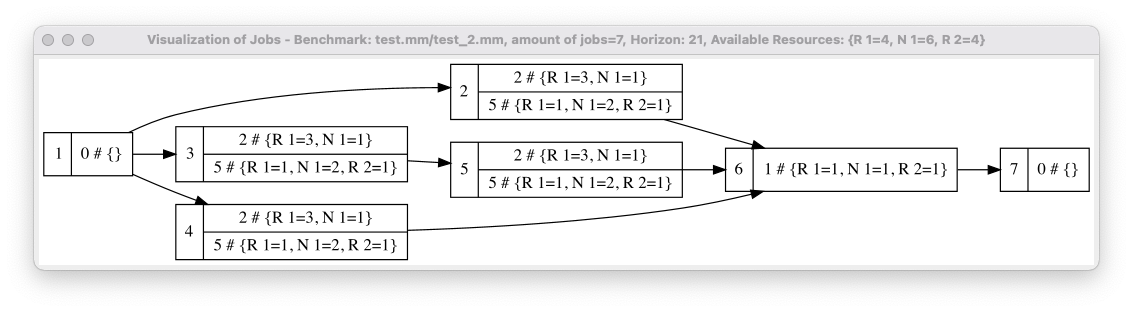
\includegraphics[width=\textwidth]{assets/img/04_Umsetzung/ScreenshotPlan.png}
    }
    \caption{Screenshot einer Projektplan-Visualisierung} 
    \label{img:visualization_projectplan}
    \source{Eigene Darstellung}
\end{figure}

Abbildung \ref{img:visualization_projectplan} stellt einen Screenshot von der Visualisierung eines beispielhaften \ac{mrcpsp}-Projektplans über den \lstinline|VisualizationService| dar. Die Darstellungsweise wurde bereits im Abschnitt \ref{subsec:MRCPSP_MM} erläutert. Für die Generierung von Projektplänen wird die Software Graphviz von \cite{att_graphviz_2021} verwendet. \lstinline|visualizeBenchmark(benchmark)| visualisiert einen Projektplan, indem jede Aktivität einen Knoten repräsentiert und diese gemäß ihrer Nachfolgebeziehungen verbunden werden. Die Positionierung der Knoten erfolgt über Graphviz automatisch.  

\begin{figure}[H]
    \centering
    \subfloat[][]{
        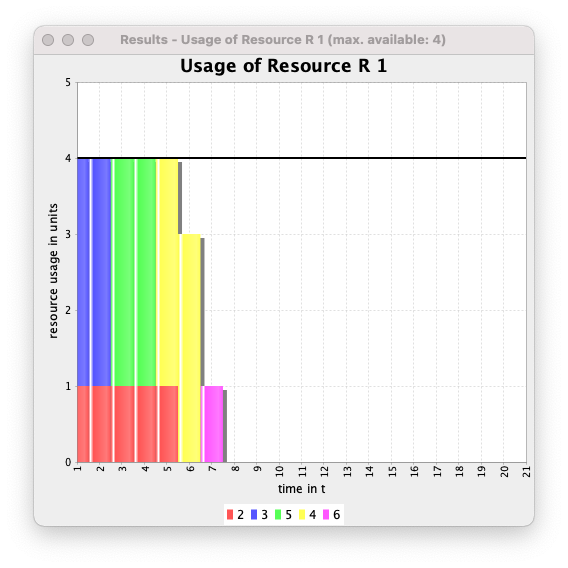
\includegraphics[width=0.51\linewidth]{assets/img/04_Umsetzung/ScreenshotR1.png}
        \label{img:visualization_schedule_a}
    }%
    \subfloat[][]{
        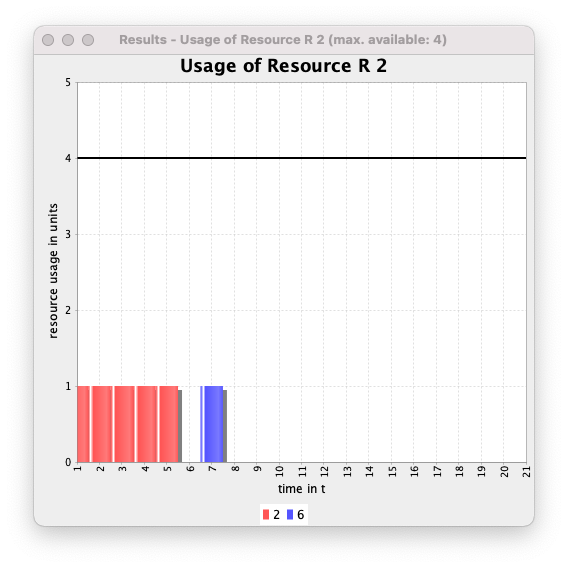
\includegraphics[width=0.51\linewidth]{assets/img/04_Umsetzung/ScreenshotR2.png}
        \label{img:visualization_schedule_b}
    }%
  
    \caption{Screenshots einer Zeitplan-Visualisierung über erneuerbare Ressourcenarten für den Projektplan aus Abbildung \ref{img:visualization_projectplan}} 
    \label{img:visualization_schedule}
    \source{Eigene Darstellung}
\end{figure}
Abbildung \ref{img:visualization_schedule} zeigt Screenshots für die Darstellung von Zeitplänen auf. Hierbei stellen Abb. \ref{img:visualization_schedule_a} und  Abb. \ref{img:visualization_schedule_b} den Ressourcenverbrauch für die erneuerbare Ressourcenart $R_1$ und $R_2$ dar. Die vertikalen Balken stellen den Ressourcenverbrauch von Aktivitäten dar, welche über die Farbe differenziert werden. Das maximale Ressourcenlimit für eine Ressource $R_k$ wird über die horizontale schwarze Linie angegeben. Folglich darf diese gemäß der \ac{mrcpsp}-Beschränkung aus Formel \ref{align:mrcpsp_constraint3} nicht überschritten werden. \\

Für den nicht-erneuerbaren Ressourcenverbrauch wird die gleiche Darstellung wie bei dem erneuerbaren Ressourcenverbrauch verwendet. Jedoch werden die nicht-erneuerbaren Ressourcen bis zum Ende des Zeitplans verwendet. Dies wird in Abbildung \ref{img:visualization_schedule_c} verdeutlicht. \\

Für die Visualisierung von Zeitplänen wird die Methode \lstinline|visualizeSchedule(schedule)| aus der Klasse \lstinline|VisualizationService| verwendet. Hierbei werden die \lstinline|XYPlot| aus der Bibliothek JFreeChart von \cite{gilbert_jfreechart_2021} verwendet, um die vertikalen Balken aufeinander stapeln zu können. 

\begin{figure}[H]
    \centering
    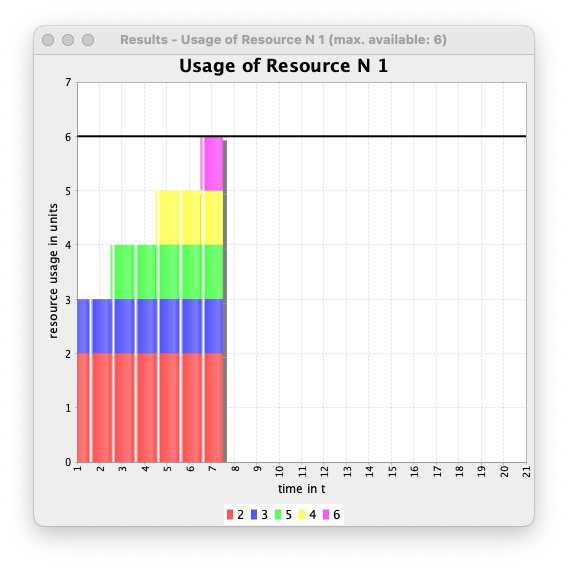
\includegraphics[width=0.47\linewidth]{assets/img/04_Umsetzung/ScreenshotN1.png}
    \caption{Screenshot einer Zeitplan-Visualisierung über nicht-erneuerbare Ressourcenarten für den Projektplan aus Abbildung \ref{img:visualization_projectplan}} 
    \label{img:visualization_schedule_c}
    \source{Eigene Darstellung}
\end{figure}
\section{Lösungsansätze} \label{sec:Loesungsansaetze}

Bereits im Abschnitt \ref{sec:AuswahlMetaheuristischenAlgorithmen}  wurden Metaheuristiken und andere Lösungsansätze selektiert, um Zeitpläne für das \ac{mrcpsp} zu finden. Als abstrakte Anlaufstelle für die Lösungsverfahren dient das Interface \lstinline|Solver|, welches eine Methode \lstinline|algorithm(...)| vorsieht. Dieses wird parametrisiert über ein \lstinline|Benchmark|-Objekt, die Anzahl an Iterationen, eine Robustheitsfunktion und eine feste Anfangsliste von Aktivitäten- und Modi, welche wiederum relevant für die reaktiven Verfahren sind. Aufgerufen wird die Methode über die einzelnen Experimente. Die konkreten Lösungsansätze implementieren diese Methode gemäß des eigentlichen Algorithmus. Für den fairen Vergleich der Algorithmen werden die Iterationen als ein Zähler von erzeugten Aktivitäts- und Moduslisten betrachtet. Das Erzeugen eines Tupels erhöht die durchlaufene Iterationen um eins. Bei einer Nachbarschaft aus fünf Elementen dementsprechend um fünf. \\

Das UML-Klassendiagramm aus Abbildung \ref{img:mrcpsp_framework_solver} zeigt das Zusammenspiel der Lösungsverfahren genauer auf. Alle aus Abschnitt \ref{sec:AuswahlMetaheuristischenAlgorithmen} selektierten Lösungsansätze werden über eine eigene Klasse repräsentiert, welche das Interface \lstinline|Solver| implementieren. Diese erzeugen über die jeweiligen Algorithmen die Aktivitäts- und Moduslisten, um so Zeitpläne über den \lstinline|SchedulerService| zu erzeugen. Insbesondere für die initialen Lösungen nutzen die Metaheuristiken den \lstinline|HeuristicDirector|, um so machbare oder sogar gute Lösungen zunächst heuristisch zu generieren. Insbesondere der \lstinline|GeneticAlgorithm| nutzt für die initiale Population unterschiedliche Prioritäts- und Selektionsregeln. \\

Ebenfalls im Abschnitt \ref{sec:AuswahlMetaheuristischenAlgorithmen} wurde eine gemeinsame Nachbarschaftsfunktion für sowohl Hill Climbing, Tabu Search als auch Simulated Annealing festgelegt. Die Funktionsweise der implementierten Nachbarschaftsfunktion $\Tilde{N}(s)$ ist in Abbildung \ref{img:implementation_neighbourhood} illustriert. Für einen zu betrachtenden Zeitplan $s$ werden stets zwei Zeitpläne in der Nachbarschaft hinzugefügt, welche eine identische Aktivitätsliste zum Basisplan aufweisen. Dennoch wird abweichend zum Basisplan ein Modus innerhalb der Modusliste umgedreht. Alle vom Basisplan aus gültigen Aktivitätsswaps werden ebenfalls einschließlich eines Moduslistenelement-Flip in der Nachbarschaft hinzugefügt. \\

\begin{figure}[H]
    \centering
    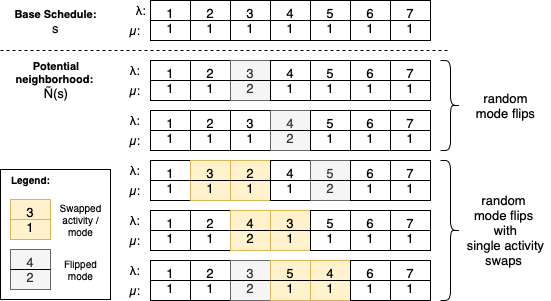
\includegraphics[width=0.84\linewidth]{assets/img/04_Umsetzung/MRCPSPNeighhbourhood.drawio.png}
    \caption{Funktionsweise der implementierten Nachbarschaftsfunktion anhand eines Beispiels für den Projektplan aus Abbildung \ref{img:visualization_projectplan}} 
    \label{img:implementation_neighbourhood}
    \source{Eigene Darstellung}
\end{figure}

In den folgenden Unterabschnitten werden die implementierten Lösungsansätze für das \ac{mrcpsp} erläutert. Zunächst wird im Abschnitt \ref{subsec:Naiv_Random} die Umsetzung der Erstellung von zufälligen Lösungen vorgestellt. Im Folgeabschnitt \ref{subsec:Hill_Climbing} wird der Hill Climbing-Algorithmus behandelt. Die Tabu Suche wird in Ausschnitt \ref{subsec:MetaheuristischeAlgorithmen_TabuSearch} erläutert, den Simulated Annealing-Algorithmus in Abschnitt \ref{subsec:MetaheuristischeAlgorithmen_SimulatedAnnealing}. Zuletzt gilt es den umgesetzten genetischen Algorithmus im Abschnitt \ref{subsec:MetaheuristischeAlgorithmen_EvolutionaereAlgorithmen} vorzustellen.

\subsection{Zufällige Lösungen} \label{subsec:Naiv_Random}

Den einfachsten Lösungsansatz stellt das Generieren von zufälligen Lösungen dar. Der \lstinline|RandomSolver| generiert mit Hilfe des \ac{ssgs} und dem \lstinline|HeuristisDirector| zunächst syntaktisch korrekte Zeitpläne. Hierbei werden als Prioritäts- und Selektionsregeln die Klassen \lstinline|RandomActvitiyHeuristic| und  \lstinline|RandomModeHeuristic| eingesetzt, welche zufällige Zahlen aus dem Intervall $[0, 10000]$ generieren. Innerhalb des Algorithmus wird in jeder Iteration überprüft, ob der gefundene Zeitplan primär die Makespan $C_{max}$ und ggf. sekundär die Robustheitsfunktion $\Omega$ verbessert und legt den besten Zeitplan fest. Dieser Algorithmus wird über eine endliche Zahl an Iterationen durchlaufen. 
\subsection{Hill Climbing} \label{subsec:Hill_Climbing}

Hill Climbing stellt mit der Klasse \lstinline|HillClimbingSolver| die Realisierung des naiven \ac{LS}-Algorithmus aus Abschnitt \ref{sec:Metaheuristiken} dar. \\

Der \ac{LS}-Algorithmus sieht eine initiale Lösung vor, welche heuristisch über zufällige Kombinationen von Prioritäts- und Selektionsregeln erstellt werden kann. Mit einer Wahrscheinlichkeit von 66\% wird beim \lstinline|HeuristicDirector| die Methode \textit{Single Sampling} ausgewählt, andernfalls werden Aktivitäts- und Moduslisten über \textit{Regret Based Biased Random Sampling} erzeugt. Es werden solange verschiedene Konstellationen von Prioritäts, Selektions- und Samplingverfahren ausprobiert, bis ein gültiger, initialer Zeitplan gefunden wurde. Insbesondere die Selektionsregel \lstinline|LRSHeuristic| eignet sich für Projekte mit einer hohen Komplexität seitens der nicht-erneuerbaren Ressourcen. Diese Art der Erstellung von initialen Lösungen wird auch bei der \ac{TS} und \ac{SA} angewandt. \\

Gemäß des erläuterten \ac{LS}-Algorithmus aus Abschnitt \ref{sec:Metaheuristiken} und der definierten Nachbarschafts(teil)funktion aus Abschnitt \ref{sec:Loesungsansaetze} wird somit iterativ die beste Lösung ausgewählt bis das lokale Optimum erreicht wurde.
\subsection{Tabu Search} \label{subsec:MetaheuristischeAlgorithmen_TabuSearch}

Bereits im Abschnitt \ref{subsec:Grundlagen_TabuSearch} wurde die Tabu Suche als eine Erweiterung des naiven \ac{LS}-Algorithmus (bzw. Hill Climbing) eingeführt. Wesentliche Komponenten, wie die generelle Funktionsweise der schrittweisen Verbesserungen, die Nachbarschaftsfunktion oder das Erzeugen der initialen Zeitpläne bleiben gleich. Folglich wurden die Implementierungen der Komponenten für die \ac{TS} aus Abschnitt \ref{subsec:Hill_Climbing} übernommen. Die Implementierung der Tabu Suche wurde in der Klasse \lstinline|TabuSearchSolver| realisiert. \\

Eins der am meist verbreitetsten (Basis-)Konzepte für die Tabu Search stellt die Tabu List dar \cite[vgl.][S. 42]{gendreau_handbook_2019}. Dieses wurde im Rahmen der eigenen Implementation aufgegriffen. Die Größe der Tabu List stellt einen Hyperparameter dar, welcher mit $|TL| = \sqrt{|J| - 2}$ versehen wurde. Des Weiteren werden neue Elemente am Anfang der Liste hinzugefügt. Die restlichen Elemente sind anschließend jeweils um eine Position verschoben, wobei das letzte Element von der Liste entfernt wird, sofern dieses nicht mehr in die Liste passt. Elemente aus der Tabu Liste werden gemäß des Konzepts nicht in der Nachbarschaft in Betracht gezogen \cite[vgl.][S. 42]{gendreau_handbook_2019}. 
\subsection{Simulated Annealing} \label{subsec:MetaheuristischeAlgorithmen_SimulatedAnnealing}
Eine Umsetzung des an der Metallurgie angelehnten \ac{SA}-Algorithmus gilt es in diesem Abschnitt zu erläutern. Die Implementierung des vorgestellten Algorithmus geschieht über die Klasse \lstinline|SimulatedAnnealingSolver|. Die folgenden Hyperparameter wurden mit den hinterlegten Werten umgesetzt, welche sich über kleinere Tests als geeignet erwiesen haben:

$T_0 = 1000$

\begin{description}
\item[Initiale Temperatur $T_0$:] Für die initiale Temperatur $T_0$ wurde ein Wert von $T_0 = 1000$ ausgewählt. 
\item[Abkühlungsrate $\alpha$:] Die Temperatur wird über die Iterationen mit einer Rate von $\alpha = 0.9$ abgekühlt. 
\end{description}

Der implementierte Algorithmus orientiert sich an dem Pseudocode aus Listing \ref{lst:simulatedannealing}. Neben der Auswahl der Hyperparameter gilt es noch die Zielfunktion $f(x)$ zu konkretisieren und die Realisierung der Auswahl der Nachbarschaftsfunktion anzupassen. 

\subsubsection*{Abweichung zur Nachbarschaftsselektion}
Im Pseudocode aus Abschnitt \ref{subsec:Grundlagen_SimulatedAnnealing} wird in einer Iteration eine zufällige Lösung aus der Nachbarschaft selektiert. In der Umsetzung für das \ac{mrcpsp} wird jedoch jedes Element einer Nachbarschaft mit einer Wahrscheinlichkeit von 50\% nicht betrachtet. Bei den restlichen zu betrachtenden Elementen einer Nachbarschaft wird das beste Element gemäß einer Funktion $f(x)$ selektiert. Dadurch wird ein Zufall gewährleistet, welcher aber nicht willkürlich die schlechtesten Lösungen selektiert. 

\subsubsection*{Realisierung der Zielfunktion $f(x)$}
Für den \ac{SA}-Algorithmus ist eine Zielfunktion $f(x)$ vorgesehen. Die Fitnessfunktion $f(x)$ des umgesetzten \ac{GA}-Algorithmus aus Abschnitt \ref{subsec:MetaheuristischeAlgorithmen_EvolutionaereAlgorithmen} wird ebenfalls für den Algorithmus eingesetzt. 
\subsection{Evolutionäre Algorithmen} \label{subsec:MetaheuristischeAlgorithmen_EvolutionaereAlgorithmen}

Einen komplexen Lösungsansatz stellen die genetischen Algorithmen, ein Teilbereich der evolutionären Algorithmen dar. In diesem Abschnitt wird die Implementierung eines genetischen Algorithmus über die Klasse \lstinline|GeneticAlgorithmSolver| erläutert. \\

Ein genetischer Algorithmus kennzeichnet sich durch eine Vielzahl an Hyperparameter. Für den implementierten Algorithmus wurden diese empirisch mit Werten definiert, welche sich innerhalb von kleineren Tests als geeignet dargestellt haben: 

\begin{itemize}
    \item \textbf{Eltern $\mu$: } Für die Anzahl der Eltern und somit auch die Populationsgröße wurde  $\mu = 40$ ausgewählt
    \item \textbf{Nachkommen $\lambda$: } Für die Anzahl der Nachkommen und somit auch die der erzeugten Zeitpläne in einer Generation wird mit $\lambda = 50$ selektiert. 
    \item \textbf{Lebensdauer $\kappa$: } Die maximale Lebensdauer eines Individuums liegt bei $\kappa = 50$ Generationen. 
    \item \textbf{Mutationsrate $\sigma$: } Die Mutationsrate wird zum Start des Algorithmus bei $\sigma = 0.06$ gesetzt und wird über eine Rechenberg Regel im Verlauf des Algorithmus angepasst. Die Rechenberg Regel wird im Verlauf der Vorstellung des Mutation Operator erläutert.
    
\end{itemize}

Bereits im Abschnitt \ref{subsec:Grundlagen_EvolutionäreAlgorithmen} wurden die unterschiedlichen Phasen über einen generischen genetischen Algorithmus aus Listing \ref{lst:ga} vorgestellt. Diese gilt es nun für das konkrete Problem des \ac{mrcpsp} und für den eigenen Algorithmus zum Finden von guten Lösungen umzusetzen.

\subsubsection*{Initiale Population}
Eine initiale Population $P$ mit $\mu = 40$ Individuen wird heuristisch erzeugt, indem verschiedene Aktivitäts- und Selektionsregeln miteinander kombiniert und solange durchlaufen werden, bis die Population vollständig ist. Dies dient dazu, unterschiedliche Lösungen mit den Vorzügen der Heuristiken zu erzeugen. Mit einer Wahrscheinlichkeit von 66\% wird als Sampling-Verfahren die Single Pass-Methode eingesetzt, andernfalls die \ac{RBRS}-Methode. Insbesondere Benchmarks mit einer hohen Komplexität an nicht-erneuerbaren Ressourcen führen dazu, dass das Erzeugen einer Population mehr Iterationen benötigt, wodurch ein Schwellwert eingeführt wird, welcher bei Überschreitung den Selektionsmodus \lstinline|LRSHeuristic| erzwingt. 

\subsubsection*{Umsetzung der Auswahl der Eltern}
Für die Crossover Operation müssen zunächst zwei Eltern $\rho = 2$ ausgewählt werden. Hierfür werden $\rho$ zufällige Einträge aus der Population entnommen. 

\subsubsection*{Umsetzung des Crossover Operator}
Bei dem eingesetzten Crossover Operator handelt es sich um den \textit{Two-Point Crossover}. Hierbei wird ein Tochterelement $D = (\lambda^D, \mu^D)$ erzeugt, wobei $\lambda^D$ und $\mu^D$ die Aktivitäts- und Moduslisten von $D$ darstellen. \\

\cite{hartmann_competitive_1998} bezieht sich in der Quelle zur Definition des Two-Point Crossovers auf das Basisproblem und somit nur auf die Aktivitätslistendarstellung. Die Anwendung auf Moduslisten durch Berücksichtigung der Positionierung ist dennoch möglich. Bei dem Two-Point Crossover werden zwei zufällige Punkte $q_1$ und $q_2$ gemäß $1 \leq q_1 < q_2 \leq J$ ausgewählt. Zudem sei $\rho_1 = (\lambda^{\rho_1}, \mu^{\rho_1})$ das Mutter- und $\rho_2 = (\lambda^{\rho_2}, \mu^{\rho_2})$ das Vaterelement. $i$ soll nun Positionen der Aktivitäts- und Modusliste aufzeigen. Die Aktivitäten und Modi von dem Mutterelement $\rho_1$ sollen zwischen $i = 0 \, ... \, q_1$ auch für das Tochterelement $D$ gelten. Als nächster Schritt wird das Vaterelement $\rho_2$ berücksichtigt. Hierbei werden die Positionen zwischen $i = q1 + 1 \, ... \, q_2$ vom Vater hergeleitet. Das Problem besteht, dass Aktivitäten doppelt auftreten können. Folglich werden Elemente zu $D$ hinzugefügt, für welche ein $k$ existiert, sodass gilt: $\lambda^{\rho_2}_k \notin \{ \lambda^D_1, ..., \lambda^D_{i-1} \}$. Zwischen $i = q_2 + 1 \, ... \, J$ wird das gleiche Prinzip wieder für das Mutterelement $\rho_1$ angewandt. Es werden die restlichen Elemente zu $D$ vom Mutterelement hinzugefügt, für welches ein $k$ existiert, sodass gilt: $\lambda^{\rho_1}_k \notin \{ \lambda^D_1, ..., \lambda^D_{i-1} \}$. Die Anwendung des Two-Point Crossover anhand eines Beispiels lässt sich in Abbildung \ref{img:twopointcrossover} illustrieren. \cite[vgl.][S. 5]{hartmann_competitive_1998}

\begin{figure}[H]
    \centering
    \noindent\makebox[\textwidth]{%
    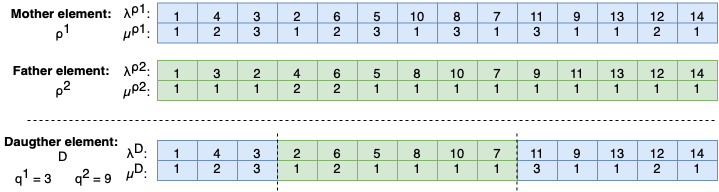
\includegraphics[width=0.93\textwidth]{assets/img/04_Umsetzung/TwoPointCrossover.drawio.png}
    }
    \caption{Beispiel des Two-Point Crossover für das MRCPSP} 
    \label{img:twopointcrossover}
    \source{Eigene Darstellung}
\end{figure}


\subsubsection*{Umsetzung des Mutation Operator}

Der implementierte Mutation Operator soll innerhalb der Aktivitäts- und Moduslisten von Nachfahren $\lambda$ leichte Änderungen realisieren. Tupels von austauschbaren Aktivitäten werden hierbei jeweils mit einer Wahrscheinlichkeit von $p_{mutation} = \sigma$ miteinander vertauscht. Mit der selben Wahrscheinlichkeit $\sigma$ zudem wird für jede Aktivität erneut ein zufälliger Modus selektiert. \\

Die Wahl einer optimalen Mutationsrate $\sigma$ stellt eine Herausforderung dar. Die Rechenberg Regel modifiziert die Mutationsrate $\sigma$ in Abhängigkeit der Erfolgsrate einer Population. Bei einer Erfolgsrate von weniger als 1/5 wird die Rate erhöht, bei 1/5 bleibt die Mutationsrate gleich. Sofern die Erfolgsrate größer als 1/5 ist, wird die Mutationsrate erhöht. \cite[vgl.][S. 24 f.]{kramer_genetic_2017} \\

Eine abgewandelte Form der Rechenberg Regel wird für den umgesetzten Algorithmus verwendet. Für die Implementierung bezieht sich die Erfolgsrate auf die Verbesserung des besten Individuums. Eine Population, die das neue beste Individuum gemäß der Fitness beinhaltet, wird als erfolgreich angesehen. Die Mutationsrate $\sigma$ wird über die folgende Formel geändert:
\begin{align*}
    \sigma = \sigma * \exp^{0.05}(a - \tfrac{1}{5}) && \text{mit }a = \begin{cases}
    0 & \text{mit Erfolgsrate} < 1/5 \\ 
    1 & \text{mit Erfolgsrate} \geq 1/5 \\ 
    \end{cases}
\end{align*}

\subsubsection*{Umsetzung des Selection Operator}
Bei dem implementierten Algorithmus handelt es sich um ein $(\mu+\lambda)-GA$, wobei die Lebensdauer einer Lösung auf $\kappa$ Generationen beschränkt ist. Wenn somit ein Individuum über $\kappa$ Generationen in die kommenden Population ausgewählt wurde, so wird die Lösung nicht mehr in der kommenden Population selektiert werden können. Es gilt das Individuum zu selektieren, für welches der Wert der Fitnessfunktion $f(x)$ am geringsten ist. 

\subsubsection*{Umsetzung der Fitnessfunktion}
Die umgesetzte Fitnessfunktion $f(x)$ orientiert sich an den Definitionen und der Priorisierungen der Zielfunktionen aus Abschnitt \ref{sec:AuswahlMetaheuristischenAlgorithmen}. Dadurch resultiert eine weitaus stärkere Gewichtung der Projektdauer $C_{max}$ im Vergleich zur Robustheit $\Omega$. Die Fitnessfunktion $f(x)$ ist gemäß dieser Gewichtung über die folgende Formel definiert:
\begin{align*}
f(x) = C_{max}(x) - \dfrac{\Omega(x)}{100}
\end{align*}


\input{pages/04_Implementierung/02_PrädiktivReaktiveMethoden}
% \section{Visualisierung der Zeitpläne} \label{sec:Visualisierung}

\chapter{Evaluation} \label{ch:Evaluation}

Das entwickelte \ac{mrcpsp}-Framework stellt mit seinen Metaheuristiken und Verfahren für den Umgang von Verspätungen die Basis zur Beantwortung der Forschungsfrage und ihrer Unterfragen dar. Dieses Kapitel nutzt die implementierten Lösungsverfahren und Methodiken und vergleicht diese auf Benchmark-Instanzen. Der Versuchsaufbau wird zunächst im Abschnitt \ref{sec:Versuchsaufbau} erläutert. Unabhängig der Verspätungsszenarien werden im Abschnitt \ref{sec:BenchmarkErgebnisse_MetaheuristischeVerfahren} die Lösungsverfahren auf unterschiedliche Benchmark-Instanzen verglichen, um so die Güte der Verfahren miteinander vergleichen zu können. Die Ergebnisse der proaktiven Methode aus dem Abschnitt \ref{sec:BenchmarkErgebnisse_NaivMethoden} stellen die Referenz für prädiktive und reaktive Methoden dar. Die Ergebnisse der Robustheitsoptimierung als prädiktive Methode werden im Abschnitt \ref{sec:BenchmarkErgebnisse_PraediktiveMethoden} und die Ergebnisse der Neuerzeugung von Zeitplänen zum Unsicherheitszeitpunkt als reaktive Methode im Abschnitt \ref{sec:BenchmarkErgebnisse_ReaktiveMethoden} aufgeführt. Anschließend werden die unterschiedlichen Methoden im Abschnitt \ref{sec:BenchmarkVergleich} miteinander verglichen. 


\section{Versuchsaufbau} \label{sec:Versuchsaufbau}

Der Versuchsaufbau erstreckt sich über die verschiedenen Experimente, welche bereits in der Umsetzung im Abschnitt \ref{sec:Experimente} erläutert wurden. Die Auswahl der Benchmark-Instanzsets wurde im Abschnitt \ref{sec:Benchmarkdatensatz} getroffen. Für die Evaluierung sind die Instanzsets m1, m2, n0, n1 und exklusiv für den Vergleich der Lösungsverfahren j20 der PSPLIB vorgesehen. \\

Die Ausführung der Experimente wurde auf zwei Computersystemen verteilt ausgeführt. Maßgeblich für die Ausführungsgeschwindigkeit ist die Prozessorleistung. Das erste System stellt ein Desktop-PC mit einem Intel\textsuperscript{\textregistered} Core\texttrademark \, i7-8700K mit 6 Kernen und 12 Threads als Prozessor dar. Das zweite System ist ein virtueller Server, welcher als Prozessor einen Intel\textsuperscript{\textregistered} Xeon\textsuperscript{\textregistered} E5-2680 v3 vorsieht, wobei von den 24 theoretischen Kernen nur 6 zur Verfügung stehen. Für den virtuellen Server lief das Bash-Startskript aus Anhang \ref{ch:Anhang} im Hintergrundmodus. 

Für die Parametrisierung der Experimente sind eine Liste von Iterationen, die Anzahl der Experimente je Solver/Iteration-Kombination und je nachdem eine Robustheitsmessung vorgesehen (vgl. Abschnitt \ref{subsec:VergleichLösungsansätze} und \ref{subsec:VergleichUnsicherheiten}).  \\

In der Literatur werden unterschiedliche Listen von Iterationen je Forschungsgegenstand verwendet. Bei dem Lösungsvariantenvergleich sind in der Literatur von \cite[S. 16]{kolisch_psplib_1997} für das (Basis) \ac{rcpsp} 1 000 und 5 000 Iterationen vorgesehen, bei \cite[S. 148]{jozefowska_simulated_2001} ist die Menge höher, nämlich 100, 500, 1 000, 5 000, 10 000, 20 000, 50 000 und 100 000, wobei in einigen Instanzsets eine Sättigung zwischen 10 000 - 20 000 Iterationen zu erkennen ist. \cite[S. 612]{wuliang_improved_2014} vergleicht die Ergebnisse verschiedener Varianten zwischen 4 000 und 6 000 Iterationen. Im Rahmen dieser Evaluierung ist somit für das Finden der (Basis-)Zeitpläne eine Liste mit 5 00, 1 000, 2 500 und 5 000 Iterationen vorgesehen. \\

Um die Qualität eines Solvers besser bestimmen zu können, werden diese je nach vorgesehener Iteration mehrfach ausgeführt und die Ergebnisse gemittelt. Die mehrfache Ausführung geschieht im Prozessor parallel (vgl. Abschnitt \ref{subsec:VergleichLösungsansätze}). In dieser Arbeit richtet sich die Anzahl der Wiederholungen nach der Menge der Rechenkerne. Hierfür wird das zweite System als Referenz verwendet und somit $n = 6$ festgelegt. Dies führt dazu, dass jeder Solver für jede Iteration sechsmal ausgeführt wird. \\

Eine Robustheitsfunktion $\Omega$ wird für den Vergleich der implementierten Lösungs-verfahren und der prädiktiven Methoden benötigt. Für den Vergleich der implementierten Lösungsverfahren wird nur die Summe der freien Puffer innerhalb eines Zeitplans betrachtet, welche über die Funktion $\Omega^{SF1}$ im Abschnitt \ref{subsec:Praediktive_Methoden} definiert ist. Die Auswahl der Robustheitsfunktion $\Omega$ für den Unsicherheitsvergleich geschieht über ein seperates Experiment, welches im Abschnitt \ref{sec:BenchmarkErgebnisse_PraediktiveMethoden} behandelt wird. \\

Im Anhang \ref{ch:Auswertungen} sind die Ergebnisse festgehalten. Durch die Vielzahl der Instanzsets wird für die Evaluierung der Fokus vermehrt auf das Set n1 festgelegt, welches eine moderate Komplexität gegenüber den anderen Instanzsets (m1, m2 und n0) aufweist. Diese gilt es dennoch in der Evaluierung zu berücksichtigen. 
 
\section{Vergleich der implementierten Lösungsverfahren} \label{sec:BenchmarkErgebnisse_MetaheuristischeVerfahren}

Die implementierten Lösungsverfahren wurden über die vollständigen Instanzsets m1, m2, n0, n1 und j20 miteinander verglichen. Tabelle \ref{tab:evaluation_solver_n1} zeigt die quantitativen Ergebnisse für das Instanzset n1 auf, während im Anhang \ref{sec:WeitereAuswertung_Metaheuristiken} die Ergebnisse der weiteren Instanzsets entnommen werden können. 
% Für den Mittelwertvergleich der abweichenden Makespans zu den Optima und für den Mittelwertvergleich der Robustheitswerte der optimalen Zeitplänen wurden Signifikanztests vollzogen. Als Signifikanztest wurde der Kruskal-Wallis-Test selektiert. Dieser Test ist für mehrere ($> 2$) unabhängige, nicht normalverteilte Gruppierungen vorgesehen. Die fünf Lösungsverfahren mit den je vier durchlaufenden Iterationen folgen keiner Normalverteilung und stellen voneinander unabhängige Gruppen dar. Das Signifikanzniveau zur Ablehnung oder Annahme der Nullhypothese $H_0$ wird auf $\alpha = 0.05$ festgelegt. 

\begin{table}[H]
\centering
\resizebox{0.91\textwidth}{!}\\
Solver & Iteration &          &  &  & \\
\midrule
RandomSolver & 500  &     6.17 & 3.47 &      14.99 & 4.11 &   100.00 &    7.69 \\
                 & 1000 &     5.30 & 3.15 &      15.21 & 5.06 &   100.00 &   10.52 \\
                 & 2500 &     4.40 & 2.76 &      15.55 & 5.34 &   100.00 &   14.91 \\
                 & 5000 &     3.76 & 2.57 &      15.66 & 5.14 &   100.00 &   19.47 \\ \hline
HillClimbing & 500  &     2.61 & 2.97 &      17.96 & 6.02 &   100.00 &   54.63 \\
                 & 1000 &     2.48 & 2.88 &      17.88 & 6.01 &   100.00 &   56.67 \\
                 & 2500 &     2.42 & 2.87 &      17.96 & 5.99 &   100.00 &   55.26 \\
                 & 5000 &     2.41 & 2.78 &      17.73 & 6.05 &   100.00 &   56.67 \\ \hline
TabuSearch & 500  &     1.85 & 2.37 &      18.00 & 6.44 &   100.00 &   64.84 \\
                 & 1000 &     1.37 & 2.00 &      17.75 & 6.64 &   100.00 &   75.35 \\
                 & 2500 &     0.94 & 1.66 &      17.54 & 6.64 &   100.00 &   83.05 \\
                 & 5000 &     0.72 & 1.43 &      17.48 & 6.69 &   100.00 &   87.76 \\ \hline
SimulatedAnnealing & 500  &     2.60 & 2.69 &      17.81 & 6.38 &   100.00 &   50.39 \\
                 & 1000 &     1.65 & 2.05 &      17.81 & 6.56 &   100.00 &   63.42 \\
                 & 2500 &     0.95 & 1.46 &      17.40 & 6.88 &   100.00 &   78.96 \\
                 & 5000 &     0.59 & 1.00 &      17.29 & 6.96 &   100.00 &   87.91 \\ \hline
GeneticAlgorithm & 500  &     2.23 & 2.35 &      17.62 & 6.47 &   100.00 &   48.04 \\
                 & 1000 &     1.03 & 1.39 &      17.09 & 6.69 &   100.00 &   73.63 \\
                 & 2500 &     0.49 & 0.88 &      17.21 & 6.72 &   100.00 &   87.13 \\
                 & 5000 &     0.39 & 0.76 &      17.30 & 6.62 &   100.00 &   91.21 \\
\bottomrule
\end{tabular}
}
\caption{Vergleich der Lösungsverfahren für das Instanzset n1}
\source{Eigene Darstellung}
\label{tab:evaluation_solver_n1}
\end{table}

Beim direkten Vergleich der Lösungsverfahren lässt sich erkennen, dass das zu-fällige Generieren von Zeitplänen die schlechteste der implementierten Varianten darstellt. Für das Instanzset n1 konnten z. B. nur 19,47 \% optimale Lösungen gefunden werden. Dieses Lösungsverfahren eignet sich jedoch für das m1-Instanzset außerordentlich gut, welches mit einer niedrigen Aktivitäts- und Modusanzahl das einfachste Instanzset der Evaluation darstellt und somit auch die geringste Anzahl an Permutationen aufweist. Hierbei konnten die besten Ergebnisse in Bezug auf die gemittelte Abweichung der Makespans, der Robustheit und der Optimum-Rate erreicht werden. Hill Climbing stellt eine Verbesserung zur zufälligen Generierung von Lösungen dar. Dennoch eignet sich das Verfahren im Vergleich auf die implementierten Metaheuristiken weniger, da sowohl die Abweichung zu den besten Makespans als auch die Rate der optimalen Lösungen am geringsten ist. Eine mögliche Begründung liegt darin, dass beim Erreichen von lokalen Optima diese nicht mehr verlassen werden können. Der integrierte Tabu Suche-Algorithmus erreicht schon mit einer geringen Anzahl an Iterationen ($i = 500$) bereits gute Ergebnisse und stellt auch mit höheren Iterationen für sowohl einfachere als auch komplexe Instanzsets solide Ergebnisse. Simulated Annealing liefert über alle Instanzsets hinweg ähnliche Ergebnisse zur Tabu Suche, jedoch mit höheren Abweichungen. Der umgesetzte genetische Algorithmus liefert ab $i = 1 000$ Iterationen in den meisten Instanzsets die besten Ergebnisse in Bezug auf die Makespanabweichung und der Optimumsrate. Abbildung \ref{fig:evaluation_solver_n1_makespan_boxplot} und \ref{fig:evaluation_solver_n1_robust_boxplot} stellen Boxplots dar, welche die weiteren deskriptiven Statistiken der einzelnen Lösungsvarianten grafisch aufführen. 

\begin{figure}[H]

    \begin{subfigure}{0.497\linewidth}
        \centering
        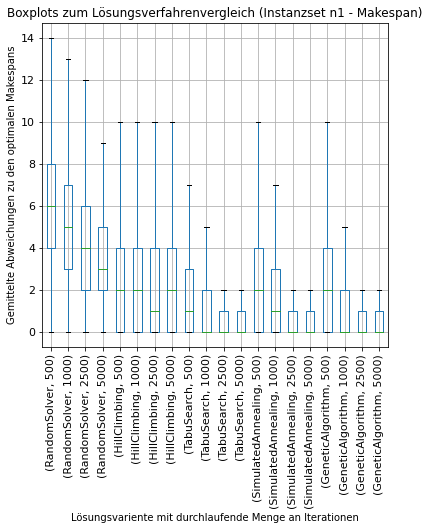
\includegraphics[width=\linewidth]{assets/img/05_Evaluation/Boxplot_n1_Makespan.png}
        \caption{Makespanabweichungen von $C_{max}$}
        \label{fig:evaluation_solver_n1_makespan_boxplot}
    \end{subfigure}
    \hfill
    \begin{subfigure}{0.497\linewidth}
        \centering
        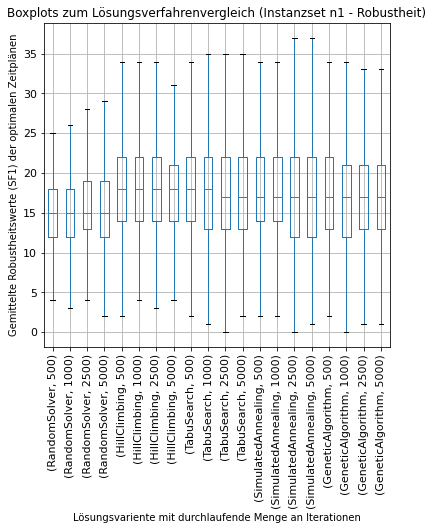
\includegraphics[width=\linewidth]{assets/img/05_Evaluation/Boxplot_n1_Robust.png}
        \caption{Robustheit $\Omega^{SF1}$}
        \label{fig:evaluation_solver_n1_robust_boxplot}
    \end{subfigure}
    
    \caption{Boxplot der implementierten Lösungsverfahren für das Instanzset m1 in Bezug auf die gemittelte a) und b)}
    \source{Eigene Darstellungen}
\end{figure}
 
\section{Benchmark-Ergebnisse der proaktiven Methoden} \label{sec:BenchmarkErgebnisse_NaivMethoden}

Die implementierten Lösungsverfahren wurden mit der jeweiligen ersten Instanz jedes Parameters der Benchmarksets m1, m2, n0 und n1 verglichen. Hierbei werden $n = 50$ zufällig generierte Unsicherheitsszenarien gemäß Abschnitt \ref{sec:Unsicherheitsszenarien} über das \lstinline|UncertaintyProactiveExperiment| durchlaufen und die gemittelten Abweichungen zu den Optima miteinander verglichen. Die selektierte proaktive Methode ignoriert Unsicherheiten. Tabelle \ref{tab:evaluation_proactive_n1} zeigt die Ergebnisse für das Instanzset n1 auf, während im Anhang \ref{sec:WeitereAuswertung_Proaktiv} die weiteren Auswertungen für die anderen Instanzsets enthalten sind. \\

{\footnotesize
\begin{longtable}{ll|rrrr|rrrr}
\toprule
\textbf{Instance set n1}                 & {} & \multicolumn{4}{c|}{Mean $\mu$} & \multicolumn{4}{c}{Std. Dev $\sigma$} \\
                & Uncertainty $p$: & 0\% & 5\% & 10\% & 20\% & 0\% & 5\% & 10\% & 20\% \\
Solver & Iteration &      &      &      &      &      &      &      &      \\
\midrule
RandomSolver & 500  & 6.30 & 7.15 & 7.91 & 9.39 & 3.50 & 3.82 & 4.02 & 4.32 \\
                 & 1000 & 5.51 & 6.40 & 7.18 & 8.69 & 3.11 & 3.47 & 3.72 & 4.11 \\
                 & 2500 & 4.66 & 5.54 & 6.34 & 7.84 & 2.83 & 3.32 & 3.63 & 3.98 \\
                 & 5000 & 3.82 & 4.70 & 5.52 & 7.03 & 2.57 & 2.89 & 3.17 & 3.55 \\ \hline
HillClimbing & 500  & 4.05 & 5.04 & 5.87 & 7.43 & 3.46 & 3.76 & 3.93 & 4.21 \\
                 & 1000 & 4.10 & 5.07 & 5.91 & 7.42 & 3.71 & 3.96 & 4.16 & 4.39 \\
                 & 2500 & 3.90 & 4.84 & 5.69 & 7.22 & 3.57 & 3.82 & 3.99 & 4.22 \\
                 & 5000 & 3.77 & 4.74 & 5.59 & 7.11 & 3.51 & 3.77 & 3.97 & 4.19 \\ \hline
TabuSearch & 500  & 1.80 & 2.77 & 3.60 & 5.13 & 2.29 & 2.72 & 2.92 & 3.27 \\
                 & 1000 & 1.23 & 2.24 & 3.11 & 4.64 & 1.86 & 2.47 & 2.77 & 3.12 \\
                 & 2500 & 0.86 & 1.85 & 2.71 & 4.24 & 1.57 & 2.12 & 2.39 & 2.75 \\
                 & 5000 & 0.56 & 1.54 & 2.39 & 3.92 & 1.14 & 1.66 & 1.95 & 2.35 \\ \hline
SimulatedAnnealing & 500  & 2.89 & 3.78 & 4.59 & 6.12 & 2.50 & 2.80 & 3.04 & 3.39 \\
                 & 1000 & 1.82 & 2.78 & 3.62 & 5.13 & 1.99 & 2.40 & 2.69 & 3.01 \\
                 & 2500 & 0.96 & 1.90 & 2.75 & 4.26 & 1.37 & 1.82 & 2.12 & 2.52 \\
                 & 5000 & 0.69 & 1.71 & 2.58 & 4.13 & 1.05 & 1.76 & 2.09 & 2.53 \\ \hline
GeneticAlgorithm & 500  & 2.28 & 3.15 & 3.94 & 5.47 & 2.30 & 2.58 & 2.81 & 3.14 \\
                 & 1000 & 1.04 & 1.92 & 2.74 & 4.24 & 1.35 & 1.78 & 2.06 & 2.43 \\
                 & 2500 & 0.57 & 1.48 & 2.31 & 3.84 & 0.90 & 1.40 & 1.70 & 2.10 \\
                 & 5000 & 0.46 & 1.40 & 2.24 & 3.79 & 0.81 & 1.45 & 1.80 & 2.22 \\
\bottomrule
\caption{Vergleich der proaktiven Lösungsverfahren auf $m=50$ unterschiedliche Unsicherheitsszenarien für das Instanzset n1. }
\label{tab:evaluation_proactive_n1}
\end{longtable}
}

\vspace*{-25px}
\begin{figure}[H]
\source{Eigene Darstellung}
\end{figure}

Über die Intensität der Unsicherheitsszenarien $p$ lassen sich wesentliche Verspät-ungen erkennen. Über $p = 0$ lassen sich die Ergebnisse der geplanten Zeitpläne ohne Verspätungen ablesen. Erst mit $p > 0$ können Verspätungen entstehen (vgl. Abschnitt \ref{sec:Unsicherheitsszenarien}). Sowohl innerhalb der Tabellen als auch über die Boxplots lassen sich je nach höherer Intensität auch höhere Verspätungen erkennen. 
 
\section{Benchmark-Ergebnisse der prädiktiven Methoden}
\label{sec:BenchmarkErgebnisse_PraediktiveMethoden}

Basierend auf dem gleichen Datensatz und Unsicherheitsszenarien vom vorherigen Abschnitt \ref{sec:BenchmarkErgebnisse_NaivMethoden} werden im Rahmen dieser prädiktiven Methode Zeitpläne gesucht, welche sowohl die Makespan $C_{max}$ minimieren, als auch die Robustheit $\Omega$ maximieren. Bereits im Abschnitt \ref{subsec:Reaktive_Methoden} wurden unterschiedliche Robustheitsmessungsfunktionen vorgestellt, wovon einige in Abschnitt \ref{subsec:ReaktiveZeitplanerstellung} in das MRPCSP-Framework integriert worden sind. \\

Zunächst gilt es die Robustheitsmessungsfunktion $\Omega$ auszuwählen, welche im Mittel die geringste Verspätung für eine Menge an zufälligen Unsicherheitsszenarien ($n = 50$) je Instanz aufweist. Tabelle \ref{tab:evaluation_robustness_n1} zeigt die implementierten Robustheitsmessungsfunktionen $\Omega$ in Kombination der Tabu-Suche auf. Im Anhang \ref{sec:WeitereAuswertung_Robustness} befinden sich für das Instanzset n1 die Resultate für die weiteren Lösungsverfahren. Als Bemessungskriterium werden die gemittelten Verspätungen zu den Basiszeitplänen festgelegt. Es lässt sich erkennen, dass Robustheitsmessungsfunktionen gegenüber keiner Robustheitsoptimierung (No-RM) geringere Projektlaufzeiten aufweisen und somit eine Möglichkeit für den Umgang mit Unsicherheiten darstellt. Insbesondere die Funktionen $\Omega^{SF2}$, $\Omega^{SF2}_{W1}$ und $\Omega^{SF3}$ stellen bessere Strategien zur Messung der Robustheit innerhalb des \ac{mrcpsp} dar. Folglich wird die Robustheitoptimierung über die Funktion $\Omega^{SF2}_{W1}$ als das zu vergleichende prädiktive Verfahren selektiert. \\

{\footnotesize
\begin{longtable}{ll|rrrr|rrrr}
\toprule
\textbf{Instance set n1}                 & {} & \multicolumn{4}{c|}{Mean $\mu$} & \multicolumn{4}{c}{Std. Dev $\sigma$} \\
\textbf{TabuSearch}                 & Uncertainty $p$: & 0\% & 5\% & 10\% & 20\% & 0\% & 5\% & 10\% & 20\% \\
Iteration & $\Omega(x)$ &      &      &      &      &      &      &      &      \\
\midrule
500  & No-RM & 0.00 & 1.01 & 1.87 & 3.46 & 0.00 & 1.45 & 1.81 & 2.28 \\
     & SF1 & 0.00 & 0.90 & 1.71 & 3.21 & 0.00 & 1.31 & 1.67 & 2.21 \\
     & SF1\_W1 & 0.00 & 0.89 & 1.72 & 3.18 & 0.00 & 1.27 & 1.68 & 2.11 \\
     & SF1\_W9 & 0.00 & 0.94 & 1.71 & 3.27 & 0.00 & 1.24 & 1.58 & 2.10 \\
     & SF2 & 0.00 & 0.86 & 1.65 & 3.14 & 0.00 & 1.21 & 1.63 & 2.08 \\
     & SF2\_W1 & 0.00 & 0.86 & 1.63 & 3.10 & 0.00 & 1.22 & 1.55 & 2.01 \\
     & SF2\_W9 & 0.00 & 0.89 & 1.70 & 3.21 & 0.00 & 1.36 & 1.78 & 2.24 \\
     & SF3 & 0.00 & 0.87 & 1.67 & 3.16 & 0.00 & 1.19 & 1.56 & 2.08 \\
     & SF3\_W1 & 0.00 & 0.86 & 1.65 & 3.15 & 0.00 & 1.18 & 1.52 & 1.96 \\
     & SF3\_W9 & 0.00 & 0.88 & 1.72 & 3.24 & 0.00 & 1.31 & 1.77 & 2.28 \\ \hline
1000 & No-RM & 0.00 & 0.98 & 1.84 & 3.35 & 0.00 & 1.38 & 1.75 & 2.23 \\
     & SF1 & 0.00 & 0.93 & 1.74 & 3.26 & 0.00 & 1.28 & 1.68 & 2.13 \\
     & SF1\_W1 & 0.00 & 0.92 & 1.77 & 3.29 & 0.00 & 1.33 & 1.79 & 2.25 \\
     & SF1\_W9 & 0.00 & 0.92 & 1.76 & 3.26 & 0.00 & 1.23 & 1.65 & 2.13 \\
     & SF2 & 0.00 & 0.89 & 1.70 & 3.20 & 0.00 & 1.34 & 1.68 & 2.16 \\
     & SF2\_W1 & 0.00 & 0.86 & 1.64 & 3.10 & 0.00 & 1.22 & 1.54 & 1.99 \\
     & SF2\_W9 & 0.00 & 0.86 & 1.67 & 3.13 & 0.00 & 1.20 & 1.60 & 1.99 \\
     & SF3 & 0.00 & 0.88 & 1.71 & 3.24 & 0.00 & 1.24 & 1.69 & 2.11 \\
     & SF3\_W1 & 0.00 & 0.89 & 1.68 & 3.22 & 0.00 & 1.25 & 1.63 & 2.11 \\
     & SF3\_W9 & 0.00 & 0.89 & 1.71 & 3.20 & 0.00 & 1.27 & 1.70 & 2.10 \\ \hline
2500 & No-RM & 0.00 & 1.02 & 1.91 & 3.46 & 0.00 & 1.38 & 1.79 & 2.26 \\
     & SF1 & 0.00 & 0.97 & 1.81 & 3.32 & 0.00 & 1.35 & 1.77 & 2.20 \\
     & SF1\_W1 & 0.00 & 0.93 & 1.71 & 3.22 & 0.00 & 1.27 & 1.60 & 2.05 \\
     & SF1\_W9 & 0.00 & 0.96 & 1.79 & 3.33 & 0.00 & 1.39 & 1.76 & 2.29 \\
     & SF2 & 0.00 & 0.85 & 1.64 & 3.17 & 0.00 & 1.18 & 1.58 & 2.07 \\
     & SF2\_W1 & 0.00 & 0.85 & 1.64 & 3.16 & 0.00 & 1.13 & 1.53 & 1.96 \\
     & SF2\_W9 & 0.00 & 0.88 & 1.69 & 3.19 & 0.00 & 1.21 & 1.64 & 2.07 \\
     & SF3 & 0.00 & 0.91 & 1.71 & 3.23 & 0.00 & 1.39 & 1.79 & 2.23 \\
     & SF3\_W1 & 0.00 & 0.90 & 1.71 & 3.24 & 0.00 & 1.28 & 1.67 & 2.15 \\
     & SF3\_W9 & 0.00 & 0.94 & 1.76 & 3.29 & 0.00 & 1.40 & 1.75 & 2.24 \\ \hline
5000 & No-RM & 0.00 & 0.99 & 1.86 & 3.39 & 0.00 & 1.20 & 1.54 & 1.94 \\
     & SF1 & 0.00 & 0.95 & 1.78 & 3.29 & 0.00 & 1.31 & 1.67 & 2.13 \\
     & SF1\_W1 & 0.00 & 0.96 & 1.77 & 3.29 & 0.00 & 1.35 & 1.74 & 2.18 \\
     & SF1\_W9 & 0.00 & 0.98 & 1.83 & 3.39 & 0.00 & 1.39 & 1.81 & 2.29 \\
     & SF2 & 0.00 & 0.85 & 1.63 & 3.12 & 0.00 & 1.14 & 1.52 & 2.02 \\
     & SF2\_W1 & 0.00 & 0.86 & 1.64 & 3.14 & 0.00 & 1.15 & 1.50 & 1.97 \\
     & SF2\_W9 & 0.00 & 0.92 & 1.71 & 3.21 & 0.00 & 1.33 & 1.67 & 2.11 \\
     & SF3 & 0.00 & 0.90 & 1.74 & 3.23 & 0.00 & 1.25 & 1.62 & 2.03 \\
     & SF3\_W1 & 0.00 & 0.91 & 1.73 & 3.23 & 0.00 & 1.28 & 1.64 & 2.06 \\
     & SF3\_W9 & 0.00 & 0.97 & 1.81 & 3.32 & 0.00 & 1.44 & 1.85 & 2.25 \\
\bottomrule
\caption{Verspätungswerte der Robustheitfunktionen $\Omega(x)$ angewendet auf die Tabu Suche für das Instanzset n1 mit $n = 50$ Unsicherheitsszenarien. }
\label{tab:evaluation_robustness_n1}
\end{longtable}
}
\vspace*{-25px}
\begin{figure}[H]
\source{Eigene Darstellung}
\end{figure}

Für alle zu untersuchenden Benchmark Sets gilt es die Robustheit über die ausgewählte Robustheitsmessungsfunktion $\Omega^{SF2}_{W1}$ zu maximieren und die Makespan $C_{max}$ zu minimieren. Dies geschieht über den \lstinline|UncertaintyPredictiveExperiment|, welcher zudem nun Basispläne über die Robustheit sekundär auswählt. Tabelle \ref{tab:evaluation_predictive_n1} zeigt die Ergebnisse des prädiktiven Verfahrens für das Instanzset n1 auf. Im Anhang \ref{sec:WeitereAuswertung_Prädiktiv} befinden sich die Ergebnisse für die weiteren Instanzsets. \\

{\footnotesize
\begin{longtable}{ll|rrrr|rrrr}
\toprule
\textbf{Instance set n1}                 & {} & \multicolumn{4}{c|}{Mean $\mu$} & \multicolumn{4}{c}{Std. Dev $\sigma$} \\
                & Uncertainty $p$: & 0\% & 5\% & 10\% & 20\% & 0\% & 5\% & 10\% & 20\% \\
Solver & Iteration &      &      &      &      &      &      &      &      \\
\midrule
RandomSolver & 500  & 6.16 & 6.97 & 7.74 & 9.21 & 3.28 & 3.55 & 3.78 & 4.16 \\
                 & 1000 & 5.43 & 6.27 & 7.04 & 8.56 & 3.16 & 3.53 & 3.78 & 4.17 \\
                 & 2500 & 4.47 & 5.28 & 6.09 & 7.54 & 2.74 & 3.04 & 3.27 & 3.63 \\
                 & 5000 & 3.90 & 4.70 & 5.48 & 6.95 & 2.60 & 2.89 & 3.10 & 3.46 \\ \hline
HillClimbing & 500  & 2.56 & 3.41 & 4.20 & 5.70 & 2.94 & 3.24 & 3.46 & 3.84 \\
                 & 1000 & 2.40 & 3.22 & 4.00 & 5.46 & 2.63 & 2.95 & 3.21 & 3.56 \\
                 & 2500 & 2.41 & 3.25 & 4.03 & 5.52 & 2.76 & 3.04 & 3.22 & 3.56 \\
                 & 5000 & 2.42 & 3.26 & 4.05 & 5.55 & 2.93 & 3.21 & 3.43 & 3.80 \\ \hline
TabuSearch & 500  & 1.60 & 2.47 & 3.27 & 4.76 & 2.17 & 2.52 & 2.79 & 3.10 \\
                 & 1000 & 1.26 & 2.12 & 2.90 & 4.38 & 1.96 & 2.30 & 2.53 & 2.91 \\
                 & 2500 & 0.86 & 1.70 & 2.49 & 4.00 & 1.55 & 1.95 & 2.23 & 2.62 \\
                 & 5000 & 0.61 & 1.46 & 2.26 & 3.75 & 1.33 & 1.71 & 1.97 & 2.34 \\ \hline
SimulatedAnnealing & 500  & 2.51 & 3.38 & 4.20 & 5.71 & 2.65 & 3.08 & 3.36 & 3.79 \\
                 & 1000 & 1.74 & 2.60 & 3.40 & 4.87 & 2.25 & 2.61 & 2.86 & 3.17 \\
                 & 2500 & 0.92 & 1.79 & 2.55 & 4.06 & 1.29 & 1.82 & 2.13 & 2.54 \\
                 & 5000 & 0.62 & 1.48 & 2.28 & 3.78 & 1.01 & 1.60 & 1.90 & 2.32 \\ \hline
GeneticAlgorithm & 500  & 2.17 & 2.99 & 3.77 & 5.25 & 2.15 & 2.42 & 2.61 & 2.94 \\
                 & 1000 & 1.09 & 1.92 & 2.70 & 4.18 & 1.37 & 1.76 & 2.03 & 2.42 \\
                 & 2500 & 0.57 & 1.42 & 2.20 & 3.67 & 0.90 & 1.43 & 1.74 & 2.16 \\
                 & 5000 & 0.43 & 1.27 & 2.05 & 3.54 & 0.80 & 1.35 & 1.69 & 2.10 \\
\bottomrule
\caption{Vergleich der prädiktiven Lösungsverfahren auf $m=50$ unterschiedliche Unsicherheitsszenarien für das Instanzset n1. }
\label{tab:evaluation_predictive_n1}
\end{longtable}
}
\vspace*{-25px}
\begin{figure}[H]
\source{Eigene Darstellung}
\end{figure}
\section{Benchmark-Ergebnisse der reaktiven Methoden} \label{sec:BenchmarkErgebnisse_ReaktiveMethoden}

Auf der identischen Datenbasis zu Abschnitt \ref{sec:BenchmarkErgebnisse_NaivMethoden} und \ref{sec:BenchmarkErgebnisse_PraediktiveMethoden} werden in diesem Abschnitt die Ergebnisse der reaktiven Methode vorgestellt. Hierbei werden zunächst Basiszeitpläne gefunden, welche die Makespan $C_{max}$ minimieren. Bei einem Verspätungszeitpunkt wird anschließend ein Folgezeitplan über eine Tabu Search gesucht, welcher die Kostenfunktion $\mathcal{C}$ aus Abschnitt \ref{subsec:Reaktive_Methoden} minimiert. Der Algorithmus nutzt als initiale Lösung den aktuellen Zeitplan und durchläuft 500 Iterationen. Die Ergebnisse der Methode für das Instanzset n1 sind in der Tabelle \ref{tab:evaluation_reactive_n1} visualisiert. Weitere Ergebnisse sind aus dem Anhang \ref{sec:WeitereAuswertung_ProaktivReaktiv} zu entnehmen. 

{\footnotesize
\begin{longtable}{ll|rrrr|rrrr}
\toprule
\textbf{Instance set n1}                 & {} & \multicolumn{4}{c|}{Mean $\mu$} & \multicolumn{4}{c}{Std. Dev $\sigma$} \\
                & Uncertainty $p$: & 0\% & 5\% & 10\% & 20\% & 0\% & 5\% & 10\% & 20\% \\
Solver & Iteration &      &      &      &      &      &      &      &      \\
\midrule
RandomSolver & 500  & 6.27 & 6.61 & 6.97 & 7.74 & 3.51 & 3.56 & 3.63 & 3.88 \\
                 & 1000 & 5.64 & 6.03 & 6.40 & 7.16 & 3.32 & 3.40 & 3.48 & 3.52 \\
                 & 2500 & 4.69 & 5.08 & 5.52 & 6.37 & 2.95 & 3.00 & 3.08 & 3.22 \\
                 & 5000 & 3.73 & 4.21 & 4.66 & 5.65 & 2.45 & 2.53 & 2.68 & 2.85 \\ \hline
HillClimbing & 500  & 3.82 & 4.39 & 4.93 & 5.98 & 3.51 & 3.47 & 3.44 & 3.41 \\
                 & 1000 & 3.84 & 4.44 & 4.93 & 6.04 & 3.38 & 3.41 & 3.41 & 3.39 \\
                 & 2500 & 3.64 & 4.21 & 4.76 & 5.84 & 3.13 & 3.15 & 3.18 & 3.18 \\
                 & 5000 & 3.94 & 4.54 & 5.10 & 6.05 & 4.06 & 4.09 & 4.11 & 3.96 \\ \hline
TabuSearch & 500  & 1.77 & 2.45 & 3.17 & 4.44 & 2.20 & 2.29 & 2.39 & 2.65 \\
                 & 1000 & 1.21 & 1.96 & 2.68 & 4.00 & 1.81 & 2.01 & 2.17 & 2.28 \\
                 & 2500 & 0.98 & 1.76 & 2.53 & 3.94 & 1.93 & 2.13 & 2.26 & 2.50 \\
                 & 5000 & 0.50 & 1.36 & 2.10 & 3.64 & 0.99 & 1.40 & 1.65 & 2.04 \\ \hline
SimulatedAnnealing & 500  & 2.91 & 3.51 & 4.02 & 5.21 & 2.55 & 2.59 & 2.68 & 2.78 \\
                 & 1000 & 1.81 & 2.52 & 3.17 & 4.42 & 2.14 & 2.33 & 2.44 & 2.70 \\
                 & 2500 & 1.05 & 1.81 & 2.54 & 3.86 & 1.41 & 1.73 & 1.90 & 2.20 \\
                 & 5000 & 0.67 & 1.51 & 2.27 & 3.67 & 1.05 & 1.48 & 1.76 & 2.02 \\ \hline
GeneticAlgorithm & 500  & 2.17 & 2.78 & 3.36 & 4.52 & 2.12 & 2.11 & 2.20 & 2.26 \\
                 & 1000 & 1.15 & 1.85 & 2.50 & 3.90 & 1.42 & 1.58 & 1.71 & 2.06 \\
                 & 2500 & 0.55 & 1.39 & 2.16 & 3.56 & 0.89 & 1.38 & 1.62 & 2.06 \\
                 & 5000 & 0.49 & 1.32 & 2.10 & 3.53 & 0.87 & 1.39 & 1.62 & 2.02 \\
\bottomrule
\caption{Vergleich der reaktiven Lösungsverfahren auf $m=50$ unterschiedliche Unsicherheitsszenarien für das Instanzset n1. }
\label{tab:evaluation_reactive_n1}
\end{longtable}
}
\vspace*{-25px}
\begin{figure}[H]
\source{Eigene Darstellung}
\end{figure}
\section{Vergleich der proaktiven, prädiktiven und reaktiven Methoden} \label{sec:BenchmarkVergleich}

Die unterschiedlichen Verfahren zum Umgang mit Unsicherheiten gilt es in diesem Abschnitt miteinander zu vergleichen. Bereits in den vorherigen Abschnitten wurden Ergebnisse der Verfahren für verschiedene Unsicherheitsszenarien aufgeführt. Für den Vergleich dienen die Ergebnisse der proaktiven Evaluation aus Abschnitt \ref{sec:BenchmarkErgebnisse_NaivMethoden} als Referenz, da Verspätungen ignoriert werden. Im Hinblick auf die Forschungsfrage aus Abschnitt \ref{sec:Ziele} gilt es zu überprüfen, wie sich der prädiktive und reaktive Ansatz für das \ac{mrcpsp} auf Basis von metaheuristischen Algorithmen bei der Erstellung von Zeitplänen in Bezug auf die Projektdauer bei Verspätungen verhält. 

\begin{table}[H]
\centering
\resizebox{0.90\textwidth}{!}{%
\begin{tabular}{ll|rrrr|rrrr|rrrr}
\toprule
                \textbf{Instance set n1} &  & \multicolumn{4}{c|}{Proactive Mean $\mu$} & \multicolumn{4}{c|}{Predictive Mean $\mu$} & \multicolumn{4}{c}{Reactive Mean $\mu$} \\
                 & Uncertainty $p$: &           0.00 & 0.05 & 0.10 & 0.20 &            0.00 & 0.05 & 0.10 & 0.20 &          0.00 & 0.05 & 0.10 & 0.20 \\
Solver & Iteration &                &      &      &      &                 &      &      &      &               &      &      &      \\
\midrule
RandomSolver & 500  &           6.30 & 7.15 & 7.91 & 9.39 &            6.16 & 6.97 & 7.74 & 9.21 &          6.27 & 6.61 & 6.97 & 7.74 \\
                 & 1000 &           5.51 & 6.40 & 7.18 & 8.69 &            5.43 & 6.27 & 7.04 & 8.56 &          5.64 & 6.03 & 6.40 & 7.16 \\
                 & 2500 &           4.66 & 5.54 & 6.34 & 7.84 &            4.47 & 5.28 & 6.09 & 7.54 &          4.69 & 5.08 & 5.52 & 6.37 \\
                 & 5000 &           3.82 & 4.70 & 5.52 & 7.03 &            3.90 & 4.70 & 5.48 & 6.95 &          3.73 & 4.21 & 4.66 & 5.65 \\ \hline
HillClimbing & 500  &           4.05 & 5.04 & 5.87 & 7.43 &            2.56 & 3.41 & 4.20 & 5.70 &          3.82 & 4.39 & 4.93 & 5.98 \\
                 & 1000 &           4.10 & 5.07 & 5.91 & 7.42 &            2.40 & 3.22 & 4.00 & 5.46 &          3.84 & 4.44 & 4.93 & 6.04 \\
                 & 2500 &           3.90 & 4.84 & 5.69 & 7.22 &            2.41 & 3.25 & 4.03 & 5.52 &          3.64 & 4.21 & 4.76 & 5.84 \\
                 & 5000 &           3.77 & 4.74 & 5.59 & 7.11 &            2.42 & 3.26 & 4.05 & 5.55 &          3.94 & 4.54 & 5.10 & 6.05 \\ \hline
TabuSearch & 500  &           1.80 & 2.77 & 3.60 & 5.13 &            1.60 & 2.47 & 3.27 & 4.76 &          1.77 & 2.45 & 3.17 & 4.44 \\
                 & 1000 &           1.23 & 2.24 & 3.11 & 4.64 &            1.26 & 2.12 & 2.90 & 4.38 &          1.21 & 1.96 & 2.68 & 4.00 \\
                 & 2500 &           0.86 & 1.85 & 2.71 & 4.24 &            0.86 & 1.70 & 2.49 & 4.00 &          0.98 & 1.76 & 2.53 & 3.94 \\
                 & 5000 &           0.56 & 1.54 & 2.39 & 3.92 &            0.61 & 1.46 & 2.26 & 3.75 &          0.50 & 1.36 & 2.10 & 3.64 \\ \hline
SimulatedAnnealing & 500  &           2.89 & 3.78 & 4.59 & 6.12 &            2.51 & 3.38 & 4.20 & 5.71 &          2.91 & 3.51 & 4.02 & 5.21 \\
                 & 1000 &           1.82 & 2.78 & 3.62 & 5.13 &            1.74 & 2.60 & 3.40 & 4.87 &          1.81 & 2.52 & 3.17 & 4.42 \\
                 & 2500 &           0.96 & 1.90 & 2.75 & 4.26 &            0.92 & 1.79 & 2.55 & 4.06 &          1.05 & 1.81 & 2.54 & 3.86 \\
                 & 5000 &           0.69 & 1.71 & 2.58 & 4.13 &            0.62 & 1.48 & 2.28 & 3.78 &          0.67 & 1.51 & 2.27 & 3.67 \\ \hline
GeneticAlgorithm & 500  &           2.28 & 3.15 & 3.94 & 5.47 &            2.17 & 2.99 & 3.77 & 5.25 &          2.17 & 2.78 & 3.36 & 4.52 \\
                 & 1000 &           1.04 & 1.92 & 2.74 & 4.24 &            1.09 & 1.92 & 2.70 & 4.18 &          1.15 & 1.85 & 2.50 & 3.90 \\
                 & 2500 &           0.57 & 1.48 & 2.31 & 3.84 &            0.57 & 1.42 & 2.20 & 3.67 &          0.55 & 1.39 & 2.16 & 3.56 \\
                 & 5000 &           0.46 & 1.40 & 2.24 & 3.79 &            0.43 & 1.27 & 2.05 & 3.54 &          0.49 & 1.32 & 2.10 & 3.53 \\
\bottomrule
\end{tabular}
}
\caption{Vergleich der Ergebnisse der pro-, prä- und reaktiven Verfahren für das Instanzset n1}
\source{Eigene Darstellung}
\label{tab:comparision_n1}
\end{table}

Tabelle \ref{tab:comparision_n1} fasst die Mittelwerte der Abweichungen zu den Optima der einzelnen Verfahren aus den vorherigen Abschnitten für das Instanzset n1 zusammen. Im Anhang \ref{sec:WeitereAuswertung_Vergleiche} befinden sich die Tabellen für die weiteren Benchmarks. \\

Diese Mittelwerte gilt es anschließend miteinander prozentual zu vergleichen. In Abbildung \ref{fig:evaluation_n1_heatmaps} werden in einer Heatmap-Darstellung die einzelnen Verfahren miteinander verglichen. Positive Werte stellen prozentuale Zunahmen und negative Werte prozentuale Abnahmen dar. 

\begin{figure}[H]

    \begin{subfigure}{0.497\linewidth}
        \centering
        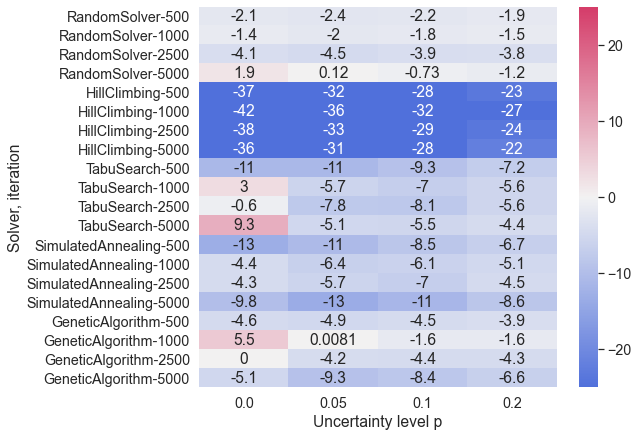
\includegraphics[width=\linewidth]{assets/img/05_Evaluation/Heatmap_n1_1.png}
        \caption{Prädiktive gegenüber proaktive Methode}
        \label{fig:evaluation_solver_n1_heatmap_1}
    \end{subfigure}
    \hfill
    \begin{subfigure}{0.497\linewidth}
        \centering
        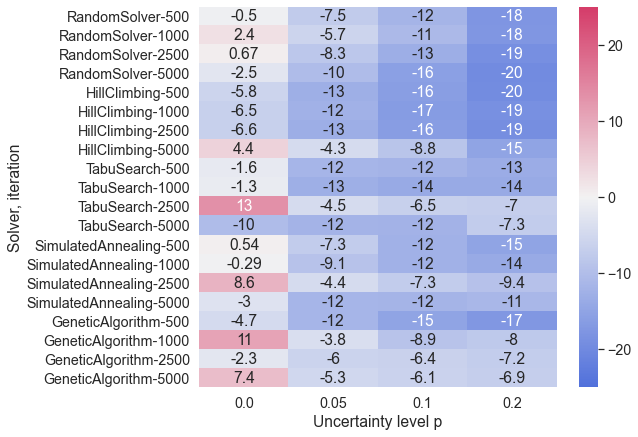
\includegraphics[width=\linewidth]{assets/img/05_Evaluation/Heatmap_n1_2.png}
        \caption{Reaktive gegenüber proaktive Methode}
        \label{fig:evaluation_solver_n1_heatmap_2}
    \end{subfigure}
    \par\bigskip 
    \begin{subfigure}{1\linewidth}
        \centering
        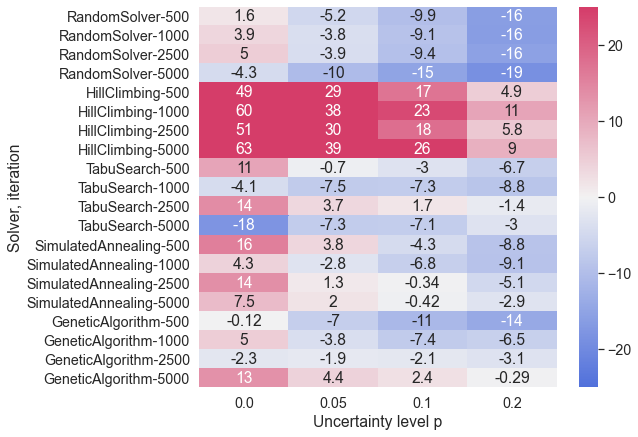
\includegraphics[width=0.5\linewidth]{assets/img/05_Evaluation/Heatmap_n1_3.png}
        \caption{Reaktive gegenüber prädiktive Methode}
        \label{fig:evaluation_solver_n1_heatmap_3}
    \end{subfigure}
    
    \caption{Heatmaps der prozentualen Abweichungen}
    \label{fig:evaluation_n1_heatmaps}
    \source{Eigene Darstellungen}
\end{figure}

Aus den Daten lässt sich erkennen, dass beim Ignorieren von Verspätungen die Abweichungen zu den Optima im Schnitt höher gegenüber der prä- und reaktiven Methode sind. Durch die Anzahl der durchlaufenden Experimente und Unsicherheitsszenarien kann bewiesen werden, dass die selektierten prädiktiven und reaktiven Verfahren einen positiven Einfluss auf die Minimierung der Verspätungen haben. \\

Innerhalb der Heatmaps lassen sich bei den Verfahren Trends über die Steigung der Unsicherheitslevel $p$ erkennen. Beim prädiktiven Ansatz über die Robustheitsoptimierung ist der beste Effekt bei $p = 0.05$ zu erkennen. Über die Erhöhung des Unsicherheitslevels sinken jedoch die prozentualen Unterschiede zum proaktiven Ansatz. Der reaktive Ansatz über das Reparieren der Zeitpläne zum Unsicherheitszeitpunkt hingegen verbessert sich über die Steigung des Unsicherheitslevels $p$, insbesondere bei einer geringen Anzahl an Iterationen bei den Basiszeitplänen. Insbesondere bei einem hohen Unsicherheitslevel ($p = 0.2$) zeigt das Verfahren deutlich höhere Unterschiede gegenüber dem proaktiven Ansatz und moderate Unterschiede gegenüber dem prädiktiven Ansatz auf. Für das \ac{mrcpsp} eignen sich prädiktive Verfahren besser für niedrigere Störungen, während reaktive Verfahren besser für komplexere Störungen geeignet sind. Dies wiederum bestätigt das, was bereits für das Basisproblem \ac{rcpsp} von \cite[vgl.][S. 405 f.]{brcic_resource_2012} über den Vergleich verschiedener Arbeiten herausgearbeitet wurde. \\

Für den direkten Vergleich von prädiktiven Verfahren gegenüber reaktiven Verfahren lassen sich jedoch Probleme feststellen, welche auf die Berechnungsdauer bezogen sind. Während prädiktive Verfahren eine feste Anzahl an Iterationen durchlaufen, werden beim reaktiven Ansatz Zeitpläne zum Unsicherheitszeitpunkt repariert, indem neue Zeitpläne gesucht werden. Hierfür wurde im Rahmen dieser Arbeit eine angepasste \acl{TS} verwendet, welche jeweils 500 Iterationen durchläuft. Dies führt dazu, dass ein weitaus höherer zeitlicher Aufwand für den reaktiven Umgang betrieben wird als gegenüber dem prädiktiven Ansatz. Basiszeitpläne, die mit einer geringen Anzahl an Iterationen gefunden wurden, profitieren von der reparierenden Tabu Suche, sodass bessere Zeitpläne gefunden werden, die bereits die Aktivitätsstörung zum Unsicherheitszeitpunkt in Betracht ziehen. Dies führt dazu, dass mit Steigung des Unsicherheitslevels die prozentualen Abweichungen bei diesen Basiszeitplänen ebenfalls steigen. Ebenfalls lassen sich bei den schwächeren Lösungsverfahren (Random Solver und Hill Climbing) in Tabelle \ref{tab:comparision_n1} deutlich geringere Differenzen zu den Basiszeitplänen feststellen. Diese Effekte gilt es bei der Interpretierung der Ergebnisse zu berücksichtigen und machen den direkten Vergleich schwieriger. \\

Bei den nachbarschaftsbasierten Algorithmen (Hill Climbing, Tabu Search und Simulated Annealing) lässt sich zudem ein weiterer Nebeneffekt innerhalb der Basiszeitpläne beim prädiktiven Ansatz erkennen. Es werden im Schnitt bessere Ergebnisse erzielt, wenn ein Algorithmus die Robustheit $\Omega$ mit berücksichtigt wird. Dies ist insbesondere in den Heatmaps aus den Abbildungen \ref{fig:evaluation_solver_n1_heatmap_1}, \ref{fig:evaluation_solver_m1_heatmap_1}, \ref{fig:evaluation_solver_m2_heatmap_1} zu erkennen. Insbesondere Hill Climbing profitiert von der Robustheitsoptimierung, sodass signifikant bessere Basiszeitpläne erzeugt wurden, welche weiterhin im Vergleich zu den Basiszeitplänen der Tabu Suche schlechter ausfallen. \\ 

Des Weiteren lässt sich in Abbildung \ref{tab:comparision_n1} erkennen, dass die Güte der Metaheuristiken auch nach Anwendung der Unsicherheitsszenarien für alle Verfahren wesentlich für die Ergebnisse sind. Ein direkter Vergleich ist somit schwierig. Im Abschnitt \ref{sec:BenchmarkErgebnisse_MetaheuristischeVerfahren} zeigte sich insbesondere der \ac{GA} als statistisch bestes der implementierten Lösungsverfahren bei der Findung von Basiszeitplänen für eine Vielzahl an Benchmark Sets. Dies und das Muster aller Lösungsvarianten ist auch nach Anwendung der Unsicherheitsszenarien zu erkennen, jedoch etwas abgeschwächter als zwischen den Basiszeitplänen. Die Wahl der Lösungsvarianten und die Anzahl der zu durchlaufenden Iterationen gilt es ebenfalls zu optimieren, um so die bestmöglichen Zeitpläne auch mit Verspätungen zu erhalten. \\

Die Intensität der Verfahren für den Umgang von Unsicherheiten hängt nicht zuletzt vom Benchmark Set ab. Während beim Benchmark Set m1 die prozentualen Abweichungen eher gering sind (vgl. Abbildung \ref{fig:evaluation_m1_heatmaps}), sind diese bei den komplexeren Sets m2 (vgl. Abbildung \ref{fig:evaluation_m2_heatmaps}), n1 (vgl. Abbildung \ref{fig:evaluation_n1_heatmaps}) und n0 (vgl. Abbildung \ref{fig:evaluation_n0_heatmaps}) stärker. 

% Welche Auswirkungenhaben präadiktive und reaktive Ansätze für das MRCPSP auf Basis von metaheuristischen Algorithmen bei der Erstellung von Zeitpläanen in Bezug auf die Projektdauer bei Verspätungen?

%%%% Die Forschungsfrage wird Mithilfe weitere Unterfragen gestützt. Welche prädiktive und reaktive Ansätze können für das MRCPSP in Kombination mit metaheuristischen Algorithmen angewandt werden? Lässt sich ein Vergleich zwischen prädiktiven und reaktiven Ansätzen auf das Ergebnis in Bezug zur Projektdauer ziehen? Welcher Einfluss haben hierbei Metaheuristiken zur Findung von \glqq guten\grqq{} Lösungen? \\ 

\chapter{Zusammenfassung und Ausblick} \label{ch:Zusammenfassung}
Der abschließende Teil dieser Masterarbeit besteht aus einem Fazit und einem Ausblick. Im Abschnitt \ref{sec:Fazit} werden die Kernthemen der Masterarbeit zusammengefasst und die wichtigsten Ergebnisse vorgestellt um die Forschungsfrage und dessen Unterfragen zu beantworten. Eine Eingliederung innerhalb des Forschungsstands wird mit einem Ausblick im Abschnitt \ref{sec:Ausblick} aufgeführt.

\section{Fazit} \label{sec:Fazit}

Das Thema der Masterarbeit basiert auf dem \ac{mrcpsp}, welches als NP-vollständig klassifiziert wurde. In dieser Arbeit wurde für das Problem ein Framework konzipiert und implementiert, welches Zeitpläne anhand von Aktivitäts- und Moduslisten erzeugt. Diese wiederum werden über eine Vielzahl an Lösungsvarianten erzeugt, um so die Zeitpläne mit der kürzesten Projektdauer $C_{max}$ zu finden. Insbesondere die implementierten Metaheuristiken \acl{TS}, \acl{SA} und \acl{GA} dienen dazu, Lösungen zu finden, welche das globale Optimum annähern. Initiale Zeitpläne wurden über das \ac{ssgs} und etabilierte heuristische Aktivitäts- und Selektionsregeln erzeugt. Die im Forschungsfeld anerkannte PSPLIB beinhaltet unterschiedliche Benchmark Sets für das \ac{mrcpsp}, die über das Framework geladen werden können. \\

Unsicherheiten, wie Aktivitätsstörungen führen zu Verspätungen bei den Projektplänen. Unsicherheitsszenarien bestehen aus Mengen von Aktivitätsstörungen, die mit einer Binomialverteilung erzeugt werden konnten. Zur Minimierung der Verspätungen wurden pro-, prä- und reaktive Verfahren konzipiert und implementiert. Um die Forschungsfrage zu beantworten, galt es diese Verfahren auf Benchmark Sets und eine Menge an zufallsgenerierten Unsicherheitsszenarien zu evaluieren. Das proaktive Verfahren und das Ignorieren von Verspätungen, dient hierbei als Referenzverfahren. Bei dem prädiktiven Verfahren wurde bereits im Suchprozess über die Metaheuristiken eine weitere Zielfunktion, nämlich die Robustheit $\Omega$ berücksichtigt, welche es zu maximieren gilt. Hierfür wurden zunächst unterschiedliche etablierte Robustheitsmessungsfunktionen selektiert und implementiert. Diese galt es anschließend auf Benchmark Sets und Unsicherheitsszenarien quantitativ zu vergleichen. Als reaktives Verfahren wurde das Reparieren von Zeitplänen zu den Unsicherheitszeitpunkten ausgewählt. Für die Reparatur wurde eine erweiterte Tabu Suche entwickelt, welche mit einer festen Anzahl an Iterationen zum Zeitpunkt reagiert. Diese minimiert die Kostenfunktion $\mathcal{C}$. Somit galt es zur Laufzeit Zeitpläne zu finden, die sich nah am Basiszeitplan orientieren und trotzdem die Verspätung zur geplanten $C_{max}$ minimiert. \\

Die Forschungsfrage befasste sich mit der Evaluierung der Auswirkungen von prädiktiven und reaktiven Verfahren auf die Projektdauer bei Verspätungen im \ac{mrcpsp}. Mithilfe eines quantitativen Vergleiches zwischen den implementierten Repräsentanten beider Verfahren gilt es die Forschungsfrage zu beantworten. Die Auswertung zeigte auf, dass sich beide Verfahren für die Verminderung der Projektverspätungen eignen. Der Grad des Unsicherheitslevels ist maßgeblich für die konkrete Auswahl des Verfahrens. Bei einem geringen Unsicherheitslevel zeigte im Schnitt das prädiktive Verfahren über die Robustheitsoptimierung eine bessere Wirkung als das reaktive Verfahren. Umgekehrt zeigte das reaktive Verfahren bei einem hohen Unsicherheitslevel eine bessere Wirkung, als das prädiktive Verfahren. Ein direkter Vergleich ist dennoch schwierig, da beim reaktiven Ansatz die Berechnungsdauer signifikant höher als beim prädiktiven Ansatz ist. Zudem eignen sich reaktive Verfahren bei Basiszeitplänen, die mit einer geringen Anzahl an Iterationen gefunden wurden. Hierbei pendeln sich über die Reparaturvorgänge womöglich bessere Zeitpläne ein und profitieren somit stark von der Güte des Reparaturalgorithmus. Reaktive Verfahren können in der Praxis insbesondere für flexible Projekte genutzt werden, während prädiktive Verfahren die Pläne über den Puffer aufrecht erhalten. Unabhängig der prädiktiven und reaktiven Verfahren stellen Metaheuristiken wesentliche Techniken zur Findung von adäquaten Basiszeitplänen dar. Es zeigte sich zudem, dass die Unterschiede zwischen den Lösungsverfahren und durchlaufenden Iterationen sowohl bei den Basiszeitplänen als auch bei den verspäteten Zeitplänen in der Relation betrachtet weiterhin vorhanden sind. 

% Welche Auswirkungen haben prädiktive und reaktive Ansätze für das MRCPSP auf Basis von metaheuristischen Algorithmen bei der Erstellung von Zeitplänen in Bezug auf die Projektdauer bei Verspätungen?

% Die Forschungsfrage wird Mithilfe weitere Unterfragen gestützt. Welche prädiktive und reaktive Ansätze können für das MRCPSP in Kombination mit metaheuristischen Algorithmen angewandt werden? Lässt sich ein Vergleich zwischen prädiktiven und reaktiven Ansätzen auf das Ergebnis in Bezug zur Projektdauer ziehen? Welcher Einfluss haben hierbei Metaheuristiken zur Findung von \glqq guten\grqq{} Lösungen?
 
\section{Ausblick} \label{sec:Ausblick}

Weiterführende Arbeiten können auf den Resultaten dieser Masterthesis aufgebaut werden. Diese Arbeit knüpft an die Erkenntnisse von \cite{brcic_resource_2012} an, in welcher für das Basisproblem \ac{rcpsp} ein Vergleich von prädiktiven und reaktiven Verfahren anhand verschiedener Publikationen vollzogen wurde. Diese Masterthesis betrachtete das \ac{mrcpsp}, eine Generalisierung des \ac{rcpsp}, und verglich quantitativ jeweils ein prädiktives und reaktives Verfahren innerhalb eines eigens implementierten Frameworks mit verschiedenen Metaheuristiken und Iterationen auf verschiedene Benchmark Sets und liefert quantitative Daten und Ergebnisse. \\

Die Erweiterbarkeit des Frameworks war im Mittelpunkt der Konzeption und Implementierung. Über die Interfaces können weitere (Meta-)Heuristiken, Metriken, Experimente oder Benchmark Loader implementiert werden. \\

Als Lösungsverfahren wurden drei Metaheuristiken selektiert, konzipiert und implementiert, nämlich \acl{TS}, \acl{SA} und \acl{GA}. Der aktuelle Trend geht neben der Entwicklung weiterer Metaheuristiken in die Richtung von hybriden Metaheuristiken. Der Einsatz von derartigen Metaheuristiken für das \ac{mrcpsp} innerhalb des Frameworks bietet weiterhin Potenzial und führt möglicherweise zu besseren Ergebnissen. Auch die Nutzung von parallelen oder verteilten Systemen innerhalb der Lösungsverfahren könnte in Zukunft mehr von Relevanz sein. \\

Bei der Robustheitsoptimierung wurde eine Vielzahl an etablierten Robustheitsmessungsfunktionen ausgewählt, implementiert und auf eine Menge von Unsicherheitsszenarien auf bestimmte Benchmark Sets miteinander verglichen. In dieser Thesis wurde somit die Robustheitsmessungsfunktion $\Omega^{SF2}_{W1}$ selektiert, welche den binären Puffer aller Aktivitäten miteinander addiert und mit der Anzahl der Nachfolger gewichtet ist. Weitere Arbeiten könnten sich auf die Selektion und Entwicklung weiterer Robustheitsmessungsfunktionen konzentrieren. \\

Im Rahmen des reaktiven Verfahrens wurden Basiszeitpläne ohne Robustheitsoptimierung zur Hand gezogen. Gemäß \cite[vgl.][S. 404 f.]{brcic_resource_2012} handelt es sich somit bei der umgesetzten Variante um ein proaktiv-reaktives Verfahren. Die Auswirkung von prädiktiv-reaktiven Verfahren, welche die Robustheitsmaximierung innerhalb der Basiszeitpläne vorsieht, kann interessante Ergebnisse liefern, welche in Folgearbeiten evaluiert werden können. \\

Zu jedem Unsicherheitszeitpunkt wurde mithilfe einer erweiterten Tabu Suche mit 500 Iterationen der kaputte Zeitplan über die Minimierung der Kostenfunktion $\mathcal{C}$ repariert. Neben Anpassungen an dem Reperaturalgorithmus können auch weitere Verfahren selektiert oder entworfen werden, um die hohe Berechnungsdauer zum Unsicherheitszeitpunkt zu senken und um das globale Minimum der Kostenfunktion besser anzunähern.

Diese Arbeit befasste sich mit Aktivitätsstörungen als einzige Unsicherheitsquelle. Folgearbeiten könnten sich auf weitere Unsicherheitsquellen, wie beispielsweise (nicht-)erneuerbare Ressourcenstörungen beziehen. \\

Die Forschungsfrage und ihre Unterfragen konnten auf quantitativer Basis beantwortet werden. Mögliche Folgearbeiten könnten den Fokus auf die qualitative Forschung legen. Die erhobenen Daten dieser Arbeit können zur Hand gezogen werden, um festzustellen, wie die Projektdauer sich über die Unsicherheitsszenarien bei Anwendung der Verfahren konkret verändert. Auch die Relevanz der Metadaten zum Projekt, wie die Anzahl der Aktivitäten, Modi, der (nicht)-erneuerbaren Ressourcen, können in einer qualitativen Erhebung genauer betrachtet werden. \\  

Diese Masterthesis bezieht sich mit dem \ac{mrcpsp} auf ein mathematisches Optimierungsproblem, welches in der Praxis, insbesondere bei der Projektplanung, Relevanz findet. Die Transformation zu Projekten in der Praxis und der einhergehenden Evaluierung von prädiktiven und reaktiven Verfahren stellt ebenfalls Forschungsbedarf dar, da sich möglicherweise weitere Anforderungen und Faktoren identifizieren lassen. In Kombination mit einer qualitativen Erhebung können hierbei neue Erkenntnisse entstehen.

% Bei den Lösungsverfahren geht der aktuelle Trend in Richtung hybride Metaheuristiken. Folglich können zukünftige Arbeiten auf die Konzeption und Entwicklung weiterer Metaheuristiken, insbesondere hybride Metaheuristiken für das (M)\ac{rcpsp} setzen. Des Weiteren können weitere Robustheitsmessfunktionen selektiert, entworfen und evaluiert werden. 

% - ! Integrierung weiterer Solver, insbesondere hybride Verfahren
% - ! Integrierung weiterer Verfahren für das reaktive Scheduling
% - ! Vergleich weiterer Robustheitsoptimierungen
% - Weitere Optimierungsprobleme oder Unterarten des RCPSP (M)RCPSP (Stochastic MMRCPSP)
% - ! Weitere prädiktive und reaktive Verfahren
% - ! Hybride Verfahren
% - Qualitative Forschung 
% -> Konkrete Analyse der Funktionsweise für reaktive Verfahren in Bezug auf die Anzahl der Aktivitäten und Modi
% -> Konkrete Analyse der Funktionsweise für die Robustheitsoptimierung in Bezug auf die Puffer 
% - ! Nutzung Parallelität innerhalb der Algorithmen
% - ! Transformation in der Realität und dessen Evaluierung


\cleardoublepage
\phantomsection
\addcontentsline{toc}{chapter}{Literaturverzeichnis} 

\bibliography{references} 

%------------
%---Anhang---
%------------

\appendix 

\chapter{Komponenten des beigefügten Materials}
\label{ch:Anhang}

Neben der vorliegenden textuellen Ausarbeitung befindet sich auf dem beigefügten Medium im Rahmen der Masterarbeit entstandenes Material. Es handelt sich hierbei um ein lokales Git-Repository, welches aus folgenden Komponenten besteht:

\begin{description}
\item[\ac{mrcpsp}-Framework] Der Rootordner entspricht das Jetbrains IntelliJ IDEA Projekt, welches über die Entwicklungsumgebung importierbar ist. Im Ordner befindet sich die \lstinline|pom.xml|, was die Maven Konfigurations-Datei darstellt, welche Metainformationen, Abhängigkeiten und Kompiliereinstellungen des \ac{mrcpsp}-Framework beinhaltet. Zudem liegt ein generierter Maven-Wrapper (mvwn und mvwn.cmd) bei. Der Java-Sourcecode und die verwendeten Benchmark Instanzen sind im Ordner \lstinline|src| vorzufinden. 

\item[Startskript der Evaluation] Im Ordner \lstinline|build| befindet sich das ausführbare Bash-Skript \lstinline|start_evaluation.sh|, welches alle Experimente gemäß Abschnitt \ref{sec:Versuchsaufbau} nacheinander startet. Das gebaute Artefakt \lstinline|mrcpsp_framework-0.0.1-SNAPSHOT.jar| liegt zudem im selben Ordner bei. Das Artefakt benötigt das Verzeichnis \lstinline|resources|, welches die Benchmark-Instanzen beinhaltet und das Verzeichnis \lstinline|results| in welchem die erhobenen CSV-Dateien gespeichert werden. Das Bash-Script kann über das Terminal mit \lstinline|bash ./start_evalution.sh| oder im Hintergrund (z. B. relevant für eine entfernte Serverinstanz) mit \lstinline|screen -S masterthesis -m -d| \lstinline|bash ./start_evalution.sh| gestartet werden.

\item[Erhobene CSV-Daten] Die erhobenen Daten befinden sich kategorisiert im Ordner \lstinline|evaluation/data|. 

\item[Jupyter Notebooks] Im Rahmen der Evaluation wurden für die verwendeten Ergebnisse, Tabellen und Abbildungen Python Skripte erstellt. Die für die Experimente jeweils zuordenbare Skripte befinden sich im Ordner \lstinline|evaluation|. Der erste Codeblock nach den Import-Direktiven definiert die Pfad-Variable der zu analysierenden CSV-Dateien. Bei der Reproduktion gilt es diese anzupassen. 

\item[\LaTeX-Code und PDF-Datei der Thesis] Diese schriftliche Ausarbeitung wurde in \LaTeX{} geschrieben. Der Sourecode und die PDF-Datei der Thesis liegen im Ordner \lstinline|thesis| vor.

\end{description}

\chapter{UML-Klassendiagramme}
% \todo{Anpassungen notwendig}

\begin{figure}[H]
    \centering
    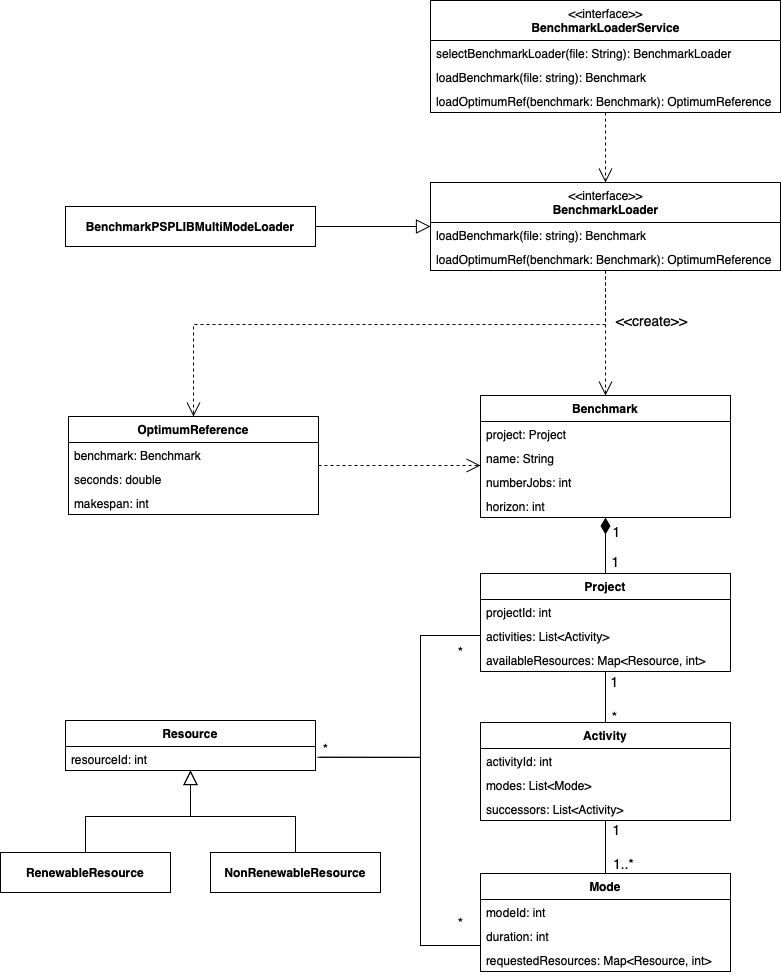
\includegraphics[width=0.85\textwidth]{assets/img/04_Umsetzung/BenchmarkLoaderInstanceSets.png}
    \caption{UML-Klassendiagramm für den Benchmark Loader} 
    \label{img:mrcpsp_framework_benchmarkloader}
    \source{Eigene Darstellung}
\end{figure}


\begin{figure}
    \centering
    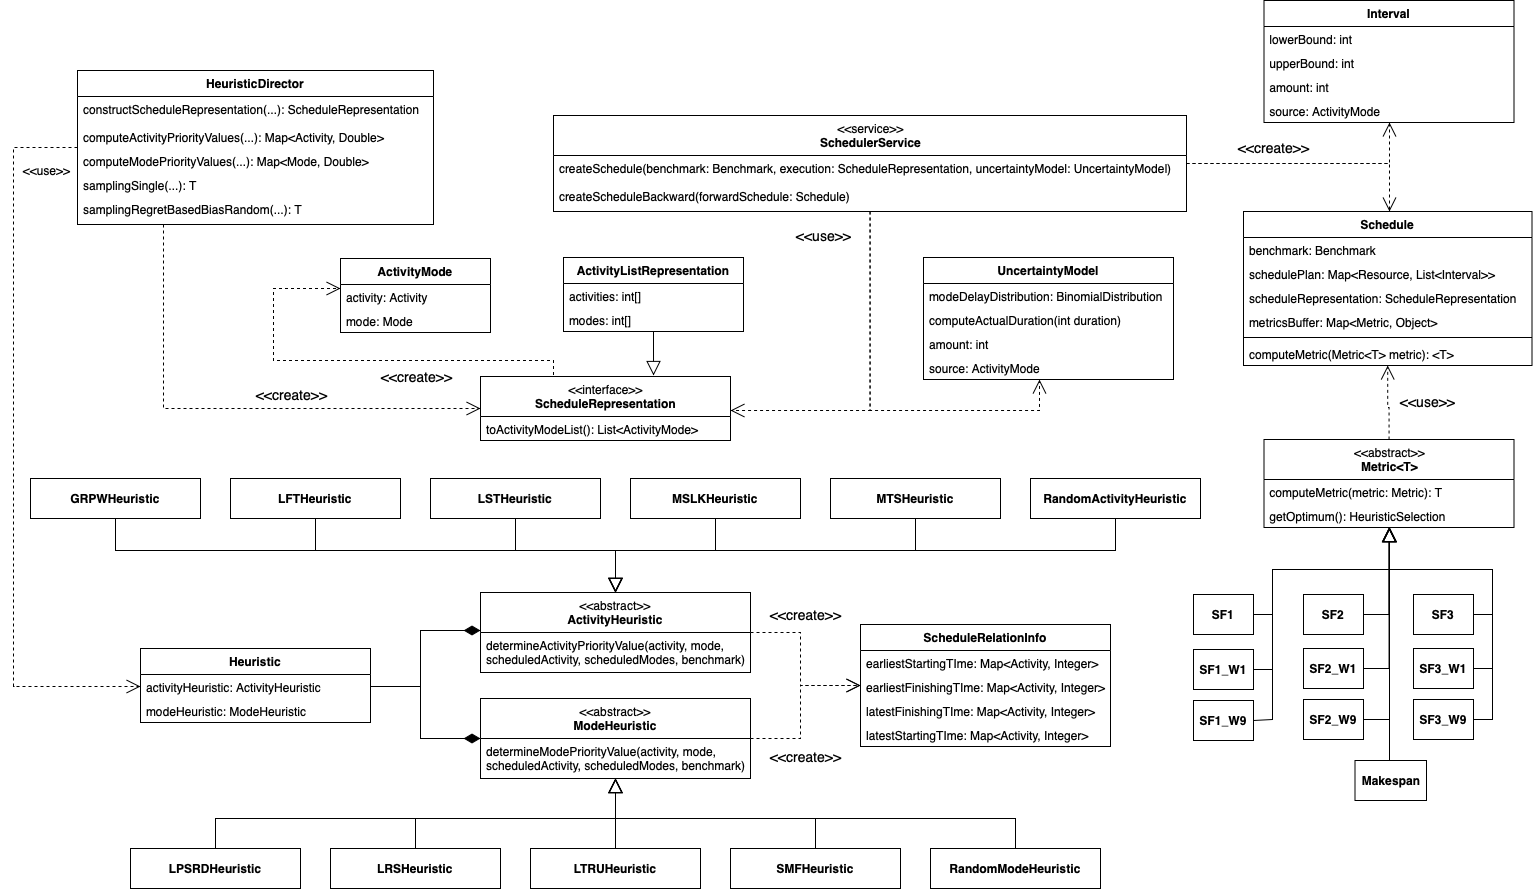
\includegraphics[angle=90,height=0.90\textheight]{assets/img/04_Umsetzung/Klassendiagramm_SchedulerHeuristiken.png}
    \caption{UML-Klassendiagramm für den Scheduler und Heuristiken} 
    \label{img:mrcpsp_framework_schedulerheuristiken}
    \source{Eigene Darstellung}
\end{figure}

\begin{figure}
    \centering
    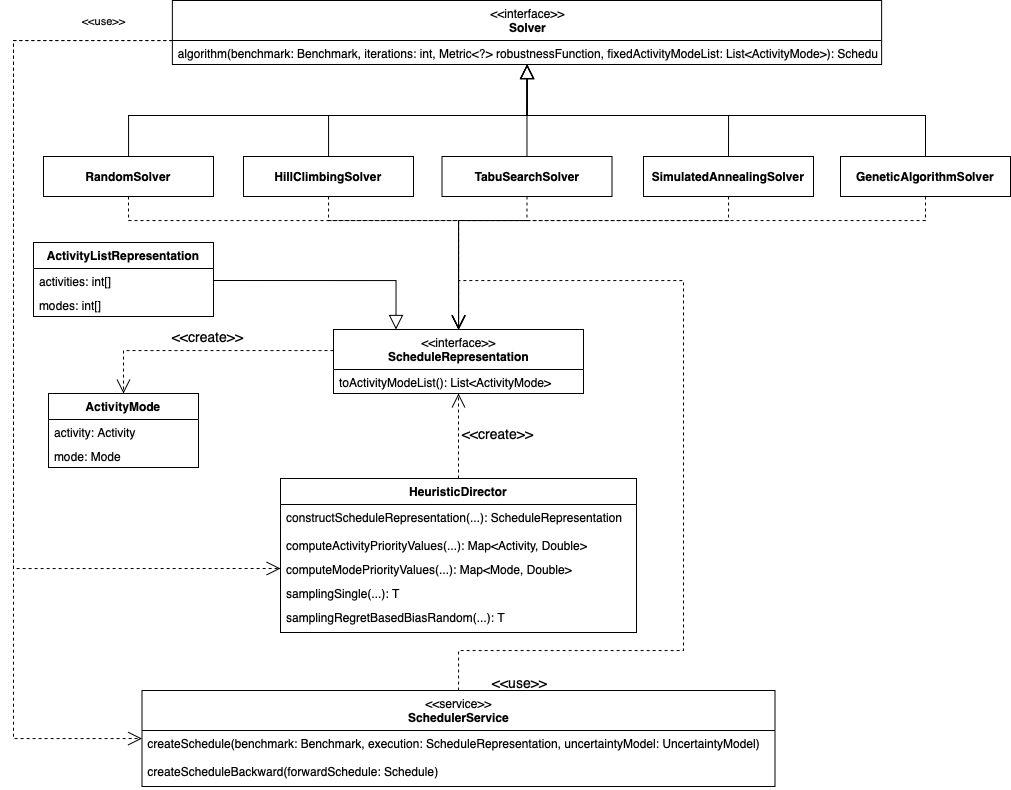
\includegraphics[width=1.06\textwidth]{assets/img/04_Umsetzung/KlassendiagrammSolver.png}
    \caption{UML-Klassendiagramm für die Solver} 
    \label{img:mrcpsp_framework_solver}
    \source{Eigene Darstellung}
\end{figure}

\begin{figure}
    \centering
    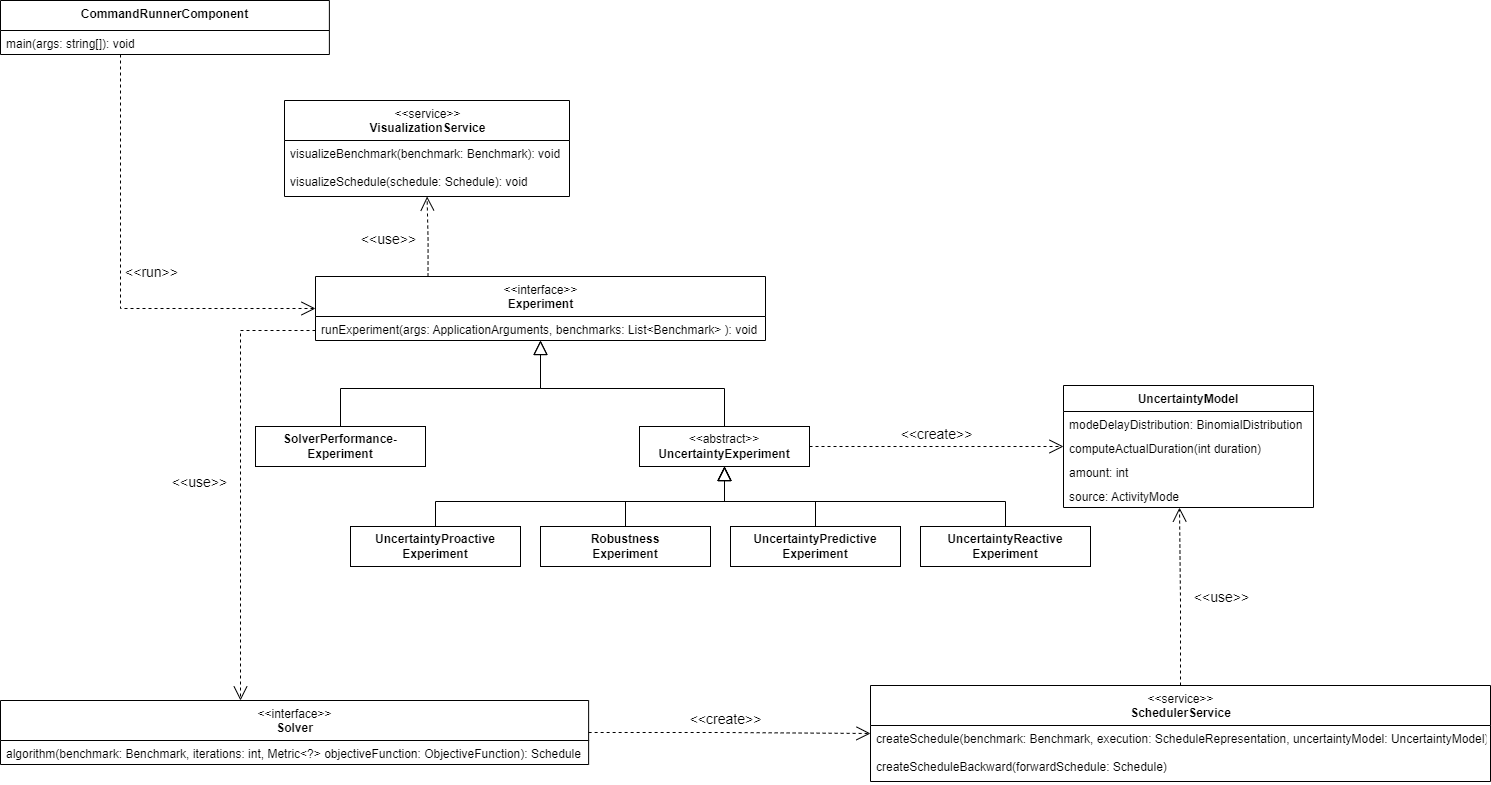
\includegraphics[angle=90,height=0.92\textheight]{assets/img/04_Umsetzung/Klassendiagramm_Experiments.drawio.png}
    \caption{UML-Klassendiagramm für die Experimente} 
    \label{img:mrcpsp_framework_experimente}
    \source{Eigene Darstellung}
\end{figure}

\chapter{Quellcode}

\begin{lstlisting}[caption={Erzeugen von Zeitplänen anhand von Aktivitäts- und Moduslisten}, label=lst:scheduler_forward, mathescape=truexinputencoding={utf8}, extendedchars=false, escapeinside=``, basicstyle=\scriptsize]
for (ActivityMode activityMode : activityModeList) {
  Mode currentMode = activityMode.getMode();
  // Create initial interval
  int potentialLowerBound = earliestStartTime.getOrDefault(activityMode.getActivity(), 0);

  // Construct the solution according the execution
  boolean solutionFound = false;
  while (!solutionFound) {
    solutionFound = true;
    for (Map.Entry<Resource, Integer> entry : currentMode.getRequestedResources().entrySet()) {
      Resource currentModeResource = entry.getKey();
      Integer currentModeAmount = entry.getValue();
      
      int resourceAvailableGeneral = benchmark.getProject().getAvailableResources()
                                .get(currentModeResource);
      int resourceAvailableOnInterval;
      
      if (currentModeResource instanceof RenewableResource) {
        int potentialUpperBound = potentialLowerBound + modeDurations.get(activityMode) - 1;

        // potential new interval that needs to be checked
        Interval potentialInterval = new Interval(potentialLowerBound,
                 potentialUpperBound,
                 currentModeAmount,
                 activityMode);

        resourceAvailableOnInterval = this.computeAvailableResourcesOnInterval(schedulePlan,
            currentModeResource, 
            potentialInterval, 
            resourceAvailableGeneral);
      } else {
        resourceAvailableOnInterval = nonRenewableResourcesLeft.get(currentModeResource);
      }

      if (currentModeAmount > resourceAvailableGeneral) {
        throw new RenewableResourceNotEnoughException();
      } else if (currentModeAmount > resourceAvailableOnInterval &&
              currentModeResource instanceof NonRenewableResource) {
            throw new NoNonRenewableResourcesLeftException(activityMode.getActivity());
      } else if (resourceAvailableOnInterval - currentModeAmount < 0) {
        solutionFound = false;
        potentialLowerBound++;
        break;
      }
    }
  }
  
  this.addInterval(activityMode,
    modeDurations.get(activityMode), 
    schedulePlan, 
    nonRenewableResourcesLeft, 
    earliestStartTime, 
    potentialLowerBound);
}
\end{lstlisting}

\begin{lstlisting}[caption={Algorithmus zur Berechnung von vorhandenen Ressourcen einer Ressourcenart für potentielles Intervall},label=lst:scheduler_computeAvailableResourcesOnInterval, mathescape=truexinputencoding={utf8}, extendedchars=false, escapeinside=``, basicstyle=\scriptsize]
private int computeAvailableResourcesOnInterval(Map<Resource, List<Interval>> scheduledPlan,
                                                Resource currentModeResource,
                                                Interval potentialInterval,
                                                int resourceAvailableGeneral) {
  int resourceAvailableOnInterval = resourceAvailableGeneral;
  List<Interval> conflictingIntervals = new ArrayList<>();

  // determine the actual resource availability on the given interval
  for (Interval intervalToCheck : scheduledPlan.get(currentModeResource)) {
    if (potentialInterval.conflictInterval(intervalToCheck)) {
      conflictingIntervals.add(intervalToCheck);
    }
  }

  // Calculate highest available resource at every timepoint
  for (int i = potentialInterval.getLowerBound(); i <= potentialInterval.getUpperBound(); i++) {
    int finalI = i;
    List<Interval> conflictingIntervalAtTimeslot = conflictingIntervals.stream()
            .filter(interval -> interval.valueInInterval(finalI)).collect(Collectors.toList());
    int availableAtTimeslot = resourceAvailableGeneral - conflictingIntervalAtTimeslot.stream()
            .map(Interval::getAmount).reduce((Integer::sum)).orElse(0);
    resourceAvailableOnInterval = Math.min(resourceAvailableOnInterval, availableAtTimeslot);
  }

  return resourceAvailableOnInterval;
}
\end{lstlisting}

\chapter{Auswertungen}
\label{ch:Auswertungen}

\section{Weitere Auswertung der implementierten Metaheuristiken}
\label{sec:WeitereAuswertung_Metaheuristiken}

\begin{table}[H]
\centering
\resizebox{\textwidth}{!}\\
Solver & Iteration &          &  &  & \\
\midrule
RandomSolver & 500  &     0.06 & 0.29 &      21.87 & 6.61 &   100.00 &   98.90 \\
                 & 1000 &     0.03 & 0.20 &      22.04 & 6.59 &   100.00 &   99.69 \\
                 & 2500 &     0.01 & 0.11 &      22.19 & 6.57 &   100.00 &  100.00 \\
                 & 5000 &     0.00 & 0.07 &      22.33 & 6.53 &   100.00 &   99.84 \\ \hline
HillClimbing & 500  &     1.83 & 2.96 &      21.11 & 6.34 &   100.00 &   63.27 \\
                 & 1000 &     1.85 & 2.98 &      21.16 & 6.38 &   100.00 &   63.42 \\
                 & 2500 &     1.85 & 2.99 &      21.09 & 6.39 &   100.00 &   62.64 \\
                 & 5000 &     1.85 & 2.97 &      21.17 & 6.39 &   100.00 &   62.32 \\ \hline
TabuSearch & 500  &     1.37 & 2.50 &      21.33 & 6.42 &   100.00 &   69.70 \\
                 & 1000 &     1.39 & 2.48 &      21.33 & 6.38 &   100.00 &   69.39 \\
                 & 2500 &     1.37 & 2.48 &      21.36 & 6.39 &   100.00 &   70.33 \\
                 & 5000 &     1.38 & 2.50 &      21.35 & 6.43 &   100.00 &   69.70 \\ \hline
SimulatedAnnealing & 500  &     1.31 & 2.43 &      21.53 & 6.30 &   100.00 &   76.77 \\ 
                 & 1000 &     1.14 & 2.21 &      21.66 & 6.30 &   100.00 &   80.38 \\
                 & 2500 &     0.88 & 1.91 &      21.90 & 6.24 &   100.00 &   84.62 \\
                 & 5000 &     0.70 & 1.71 &      21.96 & 6.28 &   100.00 &   88.70 \\ \hline
GeneticAlgorithm & 500  &     0.16 & 0.67 &      22.10 & 6.43 &   100.00 &   97.80 \\
                 & 1000 &     0.14 & 0.63 &      22.09 & 6.44 &   100.00 &   98.59 \\
                 & 2500 &     0.13 & 0.61 &      22.16 & 6.38 &   100.00 &   98.43 \\
                 & 5000 &     0.14 & 0.65 &      22.23 & 6.41 &   100.00 &   98.27 \\
\bottomrule
\end{tabular}
}
\caption{Vergleich der Lösungsverfahren für das Instanzset m1}
\source{Eigene Darstellung}
\label{tab:evaluation_solver_m1}
\end{table}


\begin{table}[H]
\centering
\resizebox{\textwidth}{!}\\
Solver & Iteration &          &  &  & \\
\midrule
RandomSolver & 500  &     2.76 & 3.43 &      17.57 & 5.87 &    99.79 &   41.04 \\
                 & 1000 &     2.26 & 3.11 &      18.23 & 5.68 &   100.00 &   47.50 \\
                 & 2500 &     1.62 & 2.59 &      18.26 & 5.97 &   100.00 &   59.38 \\
                 & 5000 &     1.30 & 2.17 &      18.45 & 6.27 &   100.00 &   63.96 \\ \hline
HillClimbing & 500  &     2.29 & 2.68 &      20.13 & 6.09 &   100.00 &   56.67 \\
                 & 1000 &     2.29 & 2.79 &      19.97 & 6.25 &   100.00 &   57.92 \\
                 & 2500 &     2.29 & 2.77 &      20.03 & 6.20 &   100.00 &   57.71 \\
                 & 5000 &     2.24 & 2.71 &      20.09 & 6.09 &   100.00 &   59.38 \\ \hline
TabuSearch & 500  &     1.65 & 2.27 &      20.39 & 6.34 &   100.00 &   70.42 \\
                 & 1000 &     1.35 & 2.03 &      20.21 & 6.28 &   100.00 &   78.12 \\
                 & 2500 &     1.05 & 1.80 &      20.20 & 6.39 &   100.00 &   86.04 \\
                 & 5000 &     0.86 & 1.71 &      20.21 & 6.42 &   100.00 &   89.38 \\ \hline
SimulatedAnnealing & 500  &     2.02 & 2.61 &      20.10 & 6.39 &   100.00 &   64.17 \\
                 & 1000 &     1.42 & 2.03 &      20.03 & 6.48 &   100.00 &   73.96 \\
                 & 2500 &     0.87 & 1.53 &      19.96 & 6.52 &   100.00 &   85.62 \\
                 & 5000 &     0.60 & 1.23 &      20.01 & 6.63 &   100.00 &   92.08 \\ \hline
GeneticAlgorithm & 500  &     1.36 & 1.74 &      19.52 & 6.50 &   100.00 &   61.25 \\
                 & 1000 &     0.64 & 1.09 &      19.62 & 6.57 &   100.00 &   82.71 \\
                 & 2500 &     0.40 & 0.84 &      19.87 & 6.48 &   100.00 &   89.17 \\
                 & 5000 &     0.33 & 0.75 &      19.76 & 6.52 &   100.00 &   92.50 \\
\bottomrule
\end{tabular}
}
\caption{Vergleich der Lösungsverfahren für das Instanzset m2}
\source{Eigene Darstellung}
\label{tab:evaluation_solver_m2}
\end{table}


\begin{table}[H]
\centering
\resizebox{\textwidth}{!}\\
Solver & Iteration &          &  &  & \\
\midrule
RandomSolver & 500  &     4.64 & 3.38 &      11.42 & 4.43 &   100.00 &   20.68 \\
                 & 1000 &     3.95 & 3.14 &      11.49 & 4.40 &   100.00 &   26.44 \\
                 & 2500 &     3.17 & 2.83 &      11.78 & 5.21 &   100.00 &   33.48 \\
                 & 5000 &     2.73 & 2.69 &      12.18 & 5.28 &   100.00 &   42.22 \\ \hline
HillClimbing & 500  &     1.30 & 2.16 &      15.94 & 6.66 &   100.00 &   78.46 \\
                 & 1000 &     1.17 & 2.01 &      16.25 & 6.91 &   100.00 &   78.46 \\
                 & 2500 &     1.09 & 1.94 &      16.02 & 6.81 &   100.00 &   80.60 \\
                 & 5000 &     1.10 & 1.96 &      16.13 & 6.81 &   100.00 &   80.60 \\  \hline
TabuSearch & 500  &     0.82 & 1.65 &      15.96 & 7.22 &   100.00 &   83.58 \\
                 & 1000 &     0.56 & 1.30 &      16.29 & 7.26 &   100.00 &   87.63 \\
                 & 2500 &     0.30 & 0.85 &      16.44 & 7.34 &   100.00 &   92.96 \\
                 & 5000 &     0.19 & 0.62 &      16.53 & 7.37 &   100.00 &   95.74 \\  \hline
SimulatedAnnealing & 500  &     1.60 & 2.25 &      15.45 & 6.80 &   100.00 &   72.71 \\
                 & 1000 &     0.83 & 1.50 &      16.01 & 7.21 &   100.00 &   80.38 \\
                 & 2500 &     0.40 & 0.90 &      16.29 & 7.54 &   100.00 &   89.77 \\
                 & 5000 &     0.23 & 0.59 &      16.34 & 7.61 &   100.00 &   92.32 \\ \hline
GeneticAlgorithm & 500  &     0.60 & 1.18 &      15.84 & 6.75 &   100.00 &   80.38 \\
                 & 1000 &     0.36 & 0.83 &      16.17 & 7.13 &   100.00 &   87.21 \\
                 & 2500 &     0.23 & 0.59 &      16.41 & 7.43 &   100.00 &   93.18 \\
                 & 5000 &     0.21 & 0.58 &      16.47 & 7.46 &   100.00 &   93.18 \\
\bottomrule
\end{tabular}
}
\caption{Vergleich der Lösungsverfahren für das Instanzset n0}
\source{Eigene Darstellung}
\label{tab:evaluation_solver_n0}
\end{table}


\begin{table}[H]
\centering
\resizebox{\textwidth}{!}\\
Solver & Iteration &          &  &  & \\
\midrule
RandomSolver & 500  &     7.18 & 9.29 &      16.19 & 4.52 &    99.28 &    2.35 \\
                 & 1000 &     7.05 & 7.17 &      18.62 & 5.42 &    99.28 &    3.25 \\
                 & 2500 &     6.25 & 5.70 &      17.94 & 5.00 &    99.28 &    6.14 \\
                 & 5000 &     5.56 & 5.39 &      18.73 & 4.86 &    99.28 &    7.40 \\ \hline
HillClimbing & 500  &     3.32 & 3.57 &      22.05 & 6.19 &   100.00 &   43.50 \\
                 & 1000 &     3.14 & 3.43 &      22.18 & 6.17 &   100.00 &   42.06 \\
                 & 2500 &     3.10 & 3.37 &      21.77 & 6.21 &   100.00 &   45.49 \\
                 & 5000 &     3.08 & 3.41 &      21.96 & 6.23 &   100.00 &   45.49 \\ \hline
TabuSearch & 500  &     2.75 & 3.13 &      22.12 & 6.57 &   100.00 &   48.92 \\
                 & 1000 &     2.26 & 2.81 &      22.20 & 6.80 &   100.00 &   55.23 \\
                 & 2500 &     1.76 & 2.46 &      22.20 & 6.86 &   100.00 &   62.82 \\
                 & 5000 &     1.40 & 2.08 &      22.12 & 7.12 &   100.00 &   70.22 \\ \hline
SimulatedAnnealing & 500  &     3.67 & 3.60 &      21.63 & 6.18 &   100.00 &   39.71 \\
                 & 1000 &     2.65 & 2.97 &      22.00 & 6.75 &   100.00 &   48.92 \\
                 & 2500 &     1.71 & 2.17 &      22.15 & 7.21 &   100.00 &   59.57 \\
                 & 5000 &     1.19 & 1.70 &      21.70 & 7.49 &   100.00 &   69.86 \\ \hline
GeneticAlgorithm & 500  &     3.43 & 3.69 &      21.25 & 6.05 &   100.00 &   38.81 \\
                 & 1000 &     1.92 & 2.21 &      21.75 & 6.78 &   100.00 &   49.10 \\
                 & 2500 &     0.97 & 1.30 &      21.53 & 7.36 &   100.00 &   66.25 \\
                 & 5000 &     0.72 & 1.09 &      21.38 & 7.48 &   100.00 &   75.99 \\
\bottomrule
\end{tabular}
}
\caption{Vergleich der Lösungsverfahren für das Instanzset j20}
\source{Eigene Darstellung}
\label{tab:evaluation_solver_j20}
\end{table}

\newpage

\section{Weitere Auswertung der proaktiven Verfahren}
\label{sec:WeitereAuswertung_Proaktiv}

{\footnotesize
\begin{longtable}{ll|rrrr|rrrr}
\toprule
\textbf{Instance set m1}                 & {} & \multicolumn{4}{c|}{Mean $\mu$} & \multicolumn{4}{c}{Std. Dev $\sigma$} \\
                & Uncertainty $p$: & 0\% & 5\% & 10\% & 20\% & 0\% & 5\% & 10\% & 20\% \\
Solver & Iteration &      &      &      &      &      &      &      &      \\
\midrule
RandomSolver & 500  & 0.05 & 0.93 & 1.75 & 3.26 & 0.24 & 1.33 & 1.76 & 2.20 \\
                 & 1000 & 0.05 & 0.91 & 1.71 & 3.20 & 0.25 & 1.31 & 1.69 & 2.15 \\
                 & 2500 & 0.03 & 0.92 & 1.73 & 3.26 & 0.16 & 1.42 & 1.80 & 2.25 \\
                 & 5000 & 0.02 & 0.92 & 1.72 & 3.22 & 0.14 & 1.35 & 1.75 & 2.21 \\ \hline
HillClimbing & 500  & 1.78 & 2.56 & 3.33 & 4.78 & 2.46 & 2.73 & 2.96 & 3.28 \\
                 & 1000 & 1.85 & 2.65 & 3.39 & 4.84 & 2.58 & 2.82 & 3.05 & 3.40 \\
                 & 2500 & 1.80 & 2.60 & 3.36 & 4.83 & 2.53 & 2.80 & 3.01 & 3.38 \\
                 & 5000 & 1.84 & 2.62 & 3.38 & 4.85 & 2.56 & 2.81 & 3.00 & 3.37 \\ \hline
TabuSearch & 500  & 1.40 & 2.21 & 2.99 & 4.47 & 2.12 & 2.43 & 2.69 & 3.06 \\
                 & 1000 & 1.34 & 2.17 & 2.94 & 4.42 & 2.07 & 2.42 & 2.67 & 3.04 \\
                 & 2500 & 1.33 & 2.16 & 2.93 & 4.44 & 2.04 & 2.40 & 2.64 & 3.06 \\
                 & 5000 & 1.37 & 2.20 & 2.97 & 4.46 & 2.16 & 2.51 & 2.74 & 3.13 \\ \hline
SimulatedAnnealing & 500  & 1.44 & 2.27 & 3.04 & 4.48 & 2.34 & 2.65 & 2.84 & 3.17 \\
                 & 1000 & 1.24 & 2.03 & 2.78 & 4.24 & 2.06 & 2.35 & 2.56 & 2.89 \\
                 & 2500 & 0.92 & 1.73 & 2.48 & 3.93 & 1.84 & 2.17 & 2.40 & 2.76 \\
                 & 5000 & 0.72 & 1.55 & 2.32 & 3.78 & 1.65 & 2.01 & 2.27 & 2.63 \\ \hline
GeneticAlgorithm & 500  & 0.14 & 1.05 & 1.84 & 3.34 & 0.59 & 1.56 & 1.94 & 2.43 \\
                 & 1000 & 0.08 & 1.01 & 1.85 & 3.36 & 0.36 & 1.61 & 2.08 & 2.58 \\
                 & 2500 & 0.09 & 1.02 & 1.84 & 3.38 & 0.43 & 1.70 & 2.13 & 2.64 \\
                 & 5000 & 0.09 & 0.97 & 1.79 & 3.31 & 0.41 & 1.45 & 1.87 & 2.38 \\
\bottomrule
\caption{Vergleich der proaktiven Lösungsverfahren auf $m=50$ unterschiedliche Unsicherheitsszenarien für das Instanzset m1. }
\label{tab:evaluation_proactive_m1}
\end{longtable}
}
\vspace*{-25px}
\begin{figure}[H]
\source{Eigene Darstellung}
\end{figure}

{\footnotesize
\begin{longtable}{ll|rrrr|rrrr}
\toprule
\textbf{Instance set m2}                 & {} & \multicolumn{4}{c|}{Mean $\mu$} & \multicolumn{4}{c}{Std. Dev $\sigma$} \\
                & Uncertainty $p$: & 0\% & 5\% & 10\% & 20\% & 0\% & 5\% & 10\% & 20\% \\
Solver & Iteration &      &      &      &      &      &      &      &      \\
\midrule
RandomSolver & 500  & 2.96 & 3.83 & 4.61 & 6.11 & 3.17 & 3.55 & 3.80 & 4.18 \\
                 & 1000 & 2.32 & 3.21 & 4.05 & 5.58 & 2.67 & 3.10 & 3.39 & 3.78 \\
                 & 2500 & 1.65 & 2.57 & 3.40 & 4.92 & 2.29 & 2.79 & 3.04 & 3.44 \\
                 & 5000 & 1.29 & 2.21 & 3.03 & 4.57 & 1.86 & 2.42 & 2.77 & 3.20 \\ \hline
HillClimbing & 500  & 2.93 & 3.78 & 4.58 & 6.00 & 3.45 & 3.71 & 3.91 & 4.15 \\
                 & 1000 & 3.04 & 3.90 & 4.67 & 6.10 & 3.50 & 3.78 & 3.95 & 4.20 \\
                 & 2500 & 2.90 & 3.77 & 4.56 & 5.99 & 3.54 & 3.83 & 4.05 & 4.31 \\
                 & 5000 & 2.87 & 3.78 & 4.58 & 6.04 & 3.40 & 3.80 & 4.02 & 4.24 \\ \hline
TabuSearch & 500  & 1.37 & 2.25 & 3.02 & 4.49 & 1.90 & 2.31 & 2.57 & 2.88 \\
                 & 1000 & 1.13 & 1.99 & 2.79 & 4.26 & 1.90 & 2.22 & 2.42 & 2.75 \\
                 & 2500 & 0.77 & 1.65 & 2.46 & 3.93 & 1.45 & 1.88 & 2.17 & 2.51 \\
                 & 5000 & 0.67 & 1.55 & 2.35 & 3.83 & 1.38 & 1.78 & 2.04 & 2.35 \\ \hline
SimulatedAnnealing & 500  & 1.89 & 2.74 & 3.50 & 4.99 & 2.31 & 2.60 & 2.80 & 3.11 \\
                 & 1000 & 1.19 & 2.08 & 2.90 & 4.35 & 1.75 & 2.17 & 2.45 & 2.73 \\
                 & 2500 & 0.74 & 1.60 & 2.38 & 3.83 & 1.25 & 1.70 & 1.93 & 2.30 \\
                 & 5000 & 0.50 & 1.41 & 2.24 & 3.67 & 1.04 & 1.73 & 2.18 & 2.48 \\ \hline
GeneticAlgorithm & 500  & 1.40 & 2.22 & 2.99 & 4.46 & 1.89 & 2.28 & 2.54 & 2.95 \\
                 & 1000 & 0.63 & 1.46 & 2.24 & 3.70 & 1.11 & 1.67 & 2.02 & 2.42 \\
                 & 2500 & 0.36 & 1.19 & 1.98 & 3.45 & 0.74 & 1.40 & 1.76 & 2.16 \\
                 & 5000 & 0.26 & 1.10 & 1.90 & 3.34 & 0.64 & 1.33 & 1.74 & 2.14 \\
\bottomrule
\caption{Vergleich der proaktiven Lösungsverfahren auf $m=50$ unterschiedliche Unsicherheitsszenarien für das Instanzset m2. }
\label{tab:evaluation_proactive_m2}
\end{longtable}
}
\vspace*{-25px}
\begin{figure}[H]
\source{Eigene Darstellung}
\end{figure}


{\footnotesize
\begin{longtable}{ll|rrrr|rrrr}
\toprule
\textbf{Instance set n0}                 & {} & \multicolumn{4}{c|}{Mean $\mu$} & \multicolumn{4}{c}{Std. Dev $\sigma$} \\
                & Uncertainty $p$: & 0\% & 5\% & 10\% & 20\% & 0\% & 5\% & 10\% & 20\% \\
Solver & Iteration &      &      &      &      &      &      &      &      \\
\midrule
RandomSolver & 500  & 4.48 & 5.30 & 6.06 & 7.51 & 3.24 & 3.58 & 3.85 & 4.29 \\
                 & 1000 & 3.82 & 4.63 & 5.40 & 6.78 & 3.07 & 3.48 & 3.80 & 4.17 \\
                 & 2500 & 3.09 & 3.95 & 4.71 & 6.15 & 2.81 & 3.29 & 3.55 & 4.08 \\
                 & 5000 & 2.62 & 3.46 & 4.22 & 5.67 & 2.62 & 2.97 & 3.26 & 3.73 \\ \hline
HillClimbing & 500  & 3.19 & 4.15 & 4.97 & 6.44 & 3.69 & 4.13 & 4.44 & 4.85 \\
                 & 1000 & 3.21 & 4.21 & 5.07 & 6.52 & 3.90 & 4.44 & 4.81 & 5.20 \\
                 & 2500 & 3.31 & 4.28 & 5.11 & 6.69 & 3.84 & 4.38 & 4.63 & 5.14 \\
                 & 5000 & 3.11 & 4.10 & 4.94 & 6.47 & 3.69 & 4.20 & 4.55 & 5.05 \\ \hline
TabuSearch & 500  & 1.01 & 1.94 & 2.71 & 4.22 & 1.85 & 2.48 & 2.80 & 3.38 \\
                 & 1000 & 0.57 & 1.47 & 2.26 & 3.70 & 1.32 & 1.95 & 2.31 & 2.80 \\
                 & 2500 & 0.24 & 1.17 & 1.97 & 3.44 & 0.73 & 1.74 & 2.13 & 2.61 \\
                 & 5000 & 0.12 & 1.07 & 1.88 & 3.33 & 0.45 & 1.54 & 1.93 & 2.38 \\ \hline
SimulatedAnnealing & 500  & 1.97 & 2.88 & 3.67 & 5.13 & 2.60 & 3.08 & 3.40 & 3.80 \\
                 & 1000 & 1.05 & 1.97 & 2.77 & 4.21 & 1.81 & 2.33 & 2.67 & 3.05 \\
                 & 2500 & 0.42 & 1.32 & 2.11 & 3.57 & 1.12 & 1.72 & 2.04 & 2.56 \\
                 & 5000 & 0.24 & 1.17 & 1.98 & 3.48 & 0.70 & 1.47 & 1.85 & 2.31 \\ \hline
GeneticAlgorithm & 500  & 0.57 & 1.38 & 2.14 & 3.54 & 1.19 & 1.72 & 2.07 & 2.54 \\
                 & 1000 & 0.26 & 1.09 & 1.83 & 3.28 & 0.67 & 1.39 & 1.74 & 2.25 \\
                 & 2500 & 0.16 & 0.99 & 1.75 & 3.18 & 0.46 & 1.25 & 1.66 & 2.17 \\
                 & 5000 & 0.13 & 0.97 & 1.70 & 3.15 & 0.44 & 1.24 & 1.58 & 2.10 \\
\bottomrule
\caption{Vergleich der proaktiven Lösungsverfahren auf $m=50$ unterschiedliche Unsicherheitsszenarien für das Instanzset n0. }
\label{tab:evaluation_proactive_n0}
\end{longtable}
}
\vspace*{-25px}
\begin{figure}[H]
\source{Eigene Darstellung}
\end{figure}

\newpage

\section{Weitere Auswertung der prädiktiven Verfahren}
\label{sec:WeitereAuswertung_Prädiktiv}

\subsection{Vergleich der unterschiedlichen Robustheitsmessungen}
\label{sec:WeitereAuswertung_Robustness}

{\fontsize{9.5}{10.5} \selectfont
\begin{longtable}{ll|rrrr|rrrr}
\toprule
\textbf{Instance set n1}                 & {} & \multicolumn{4}{c|}{Mean $\mu$} & \multicolumn{4}{c}{Std. Dev $\sigma$} \\
\textbf{RandomSolver}                 & Uncertainty $p$: & 0\% & 5\% & 10\% & 20\% & 0\% & 5\% & 10\% & 20\% \\
Iteration & $\Omega(x)$ &      &      &      &      &      &      &      &      \\
\midrule
500  & No-RM & 0.00 & 0.82 & 1.62 & 3.09 & 0.00 & 1.16 & 1.62 & 2.07 \\
     & SF1 & 0.00 & 0.85 & 1.65 & 3.12 & 0.00 & 1.26 & 1.72 & 2.23 \\
     & SF1\_W1 & 0.00 & 0.83 & 1.61 & 3.06 & 0.00 & 1.24 & 1.65 & 2.11 \\
     & SF1\_W9 & 0.00 & 0.83 & 1.61 & 3.11 & 0.00 & 1.18 & 1.58 & 2.05 \\
     & SF2 & 0.00 & 0.83 & 1.59 & 3.03 & 0.00 & 1.22 & 1.59 & 2.06 \\
     & SF2\_W1 & 0.00 & 0.82 & 1.56 & 3.05 & 0.00 & 1.27 & 1.65 & 2.12 \\
     & SF2\_W9 & 0.00 & 0.84 & 1.62 & 3.08 & 0.00 & 1.32 & 1.71 & 2.17 \\
     & SF3 & 0.00 & 0.85 & 1.63 & 3.15 & 0.00 & 1.31 & 1.71 & 2.22 \\
     & SF3\_W1 & 0.00 & 0.83 & 1.62 & 3.06 & 0.00 & 1.22 & 1.65 & 2.06 \\
     & SF3\_W9 & 0.00 & 0.80 & 1.58 & 3.04 & 0.00 & 1.07 & 1.46 & 1.90 \\ \hline
1000 & No-RM & 0.00 & 0.88 & 1.69 & 3.22 & 0.00 & 1.32 & 1.73 & 2.22 \\
     & SF1 & 0.00 & 0.81 & 1.60 & 3.09 & 0.00 & 1.18 & 1.63 & 2.13 \\
     & SF1\_W1 & 0.00 & 0.89 & 1.69 & 3.23 & 0.00 & 1.39 & 1.75 & 2.26 \\
     & SF1\_W9 & 0.00 & 0.85 & 1.65 & 3.13 & 0.00 & 1.29 & 1.70 & 2.18 \\
     & SF2 & 0.00 & 0.81 & 1.58 & 3.04 & 0.00 & 1.18 & 1.56 & 2.00 \\
     & SF2\_W1 & 0.00 & 0.79 & 1.54 & 3.02 & 0.00 & 1.06 & 1.45 & 1.95 \\
     & SF2\_W9 & 0.00 & 0.83 & 1.62 & 3.07 & 0.00 & 1.18 & 1.59 & 2.03 \\
     & SF3 & 0.00 & 0.82 & 1.56 & 3.04 & 0.00 & 1.17 & 1.48 & 2.02 \\
     & SF3\_W1 & 0.00 & 0.81 & 1.60 & 3.08 & 0.00 & 1.12 & 1.50 & 1.99 \\
     & SF3\_W9 & 0.00 & 0.81 & 1.61 & 3.08 & 0.00 & 1.16 & 1.60 & 2.06 \\ \hline
2500 & No-RM & 0.00 & 0.86 & 1.67 & 3.19 & 0.00 & 1.24 & 1.64 & 2.18 \\
     & SF1 & 0.00 & 0.82 & 1.61 & 3.07 & 0.00 & 1.19 & 1.57 & 1.98 \\
     & SF1\_W1 & 0.00 & 0.87 & 1.66 & 3.16 & 0.00 & 1.22 & 1.65 & 2.06 \\
     & SF1\_W9 & 0.00 & 0.86 & 1.65 & 3.14 & 0.00 & 1.28 & 1.65 & 2.12 \\
     & SF2 & 0.00 & 0.82 & 1.58 & 3.05 & 0.00 & 1.24 & 1.61 & 2.07 \\
     & SF2\_W1 & 0.00 & 0.81 & 1.59 & 3.09 & 0.00 & 1.14 & 1.55 & 2.02 \\
     & SF2\_W9 & 0.00 & 0.82 & 1.60 & 3.06 & 0.00 & 1.17 & 1.57 & 2.04 \\
     & SF3 & 0.00 & 0.83 & 1.62 & 3.07 & 0.00 & 1.16 & 1.53 & 1.96 \\
     & SF3\_W1 & 0.00 & 0.83 & 1.63 & 3.11 & 0.00 & 1.21 & 1.70 & 2.14 \\
     & SF3\_W9 & 0.00 & 0.87 & 1.67 & 3.16 & 0.00 & 1.19 & 1.58 & 2.02 \\ \hline
5000 & No-RM & 0.00 & 0.89 & 1.70 & 3.18 & 0.00 & 1.27 & 1.63 & 2.09 \\
     & SF1 & 0.00 & 0.86 & 1.67 & 3.17 & 0.00 & 1.21 & 1.64 & 2.04 \\
     & SF1\_W1 & 0.00 & 0.86 & 1.65 & 3.15 & 0.00 & 1.25 & 1.66 & 2.11 \\
     & SF1\_W9 & 0.00 & 0.84 & 1.64 & 3.15 & 0.00 & 1.17 & 1.57 & 2.02 \\
     & SF2 & 0.00 & 0.83 & 1.62 & 3.11 & 0.00 & 1.23 & 1.60 & 2.12 \\
     & SF2\_W1 & 0.00 & 0.83 & 1.61 & 3.09 & 0.00 & 1.14 & 1.53 & 1.98 \\
     & SF2\_W9 & 0.00 & 0.87 & 1.68 & 3.20 & 0.00 & 1.24 & 1.63 & 2.14 \\
     & SF3 & 0.00 & 0.84 & 1.63 & 3.12 & 0.00 & 1.21 & 1.60 & 2.04 \\
     & SF3\_W1 & 0.00 & 0.84 & 1.64 & 3.15 & 0.00 & 1.17 & 1.60 & 2.04 \\
     & SF3\_W9 & 0.00 & 0.91 & 1.72 & 3.23 & 0.00 & 1.41 & 1.82 & 2.29 \\
\bottomrule
\caption{Verspätungswerte der Robustheitfunktionen $\Omega(x)$ angewendet auf den \acs{RS} für das Instanzset n1 mit $n = 50$ Unsicherheitsszenarien. }
\label{tab:evaluation_robustness_n1_ra}
\end{longtable}
}
\vspace*{-25px}
\begin{figure}[H]
\source{Eigene Darstellung}
\end{figure}

\newpage

{\fontsize{10}{11} \selectfont
\begin{longtable}{ll|rrrr|rrrr}
\toprule
\textbf{Instance set n1}                 & {} & \multicolumn{4}{c|}{Mean $\mu$} & \multicolumn{4}{c}{Std. Dev $\sigma$} \\
\textbf{HillClimbing}                 & Uncertainty $p$: & 0\% & 5\% & 10\% & 20\% & 0\% & 5\% & 10\% & 20\% \\
Iteration & $\Omega(x)$ &      &      &      &      &      &      &      &      \\
\midrule
500  & No-RM & 0.00 & 0.97 & 1.81 & 3.33 & 0.00 & 1.27 & 1.62 & 2.03 \\
     & SF1 & 0.00 & 0.92 & 1.72 & 3.26 & 0.00 & 1.41 & 1.78 & 2.28 \\
     & SF1\_W1 & 0.00 & 0.87 & 1.68 & 3.17 & 0.00 & 1.21 & 1.63 & 2.11 \\
     & SF1\_W9 & 0.00 & 0.93 & 1.75 & 3.28 & 0.00 & 1.35 & 1.75 & 2.25 \\
     & SF2 & 0.00 & 0.87 & 1.64 & 3.16 & 0.00 & 1.32 & 1.76 & 2.25 \\
     & SF2\_W1 & 0.00 & 0.85 & 1.61 & 3.13 & 0.00 & 1.26 & 1.66 & 2.17 \\
     & SF2\_W9 & 0.00 & 0.82 & 1.59 & 3.09 & 0.00 & 1.20 & 1.59 & 2.11 \\
     & SF3 & 0.00 & 0.91 & 1.75 & 3.30 & 0.00 & 1.43 & 1.86 & 2.39 \\
     & SF3\_W1 & 0.00 & 0.87 & 1.66 & 3.19 & 0.00 & 1.23 & 1.62 & 2.12 \\
     & SF3\_W9 & 0.00 & 0.89 & 1.68 & 3.21 & 0.00 & 1.28 & 1.65 & 2.20 \\ \hline
1000 & No-RM & 0.00 & 0.96 & 1.80 & 3.34 & 0.00 & 1.16 & 1.52 & 2.02 \\
     & SF1 & 0.00 & 0.94 & 1.78 & 3.31 & 0.00 & 1.39 & 1.79 & 2.29 \\
     & SF1\_W1 & 0.00 & 0.88 & 1.68 & 3.19 & 0.00 & 1.16 & 1.57 & 2.05 \\
     & SF1\_W9 & 0.00 & 0.90 & 1.71 & 3.22 & 0.00 & 1.32 & 1.72 & 2.23 \\
     & SF2 & 0.00 & 0.82 & 1.61 & 3.07 & 0.00 & 1.13 & 1.54 & 2.01 \\
     & SF2\_W1 & 0.00 & 0.83 & 1.59 & 3.13 & 0.00 & 1.16 & 1.52 & 2.10 \\
     & SF2\_W9 & 0.00 & 0.87 & 1.68 & 3.18 & 0.00 & 1.28 & 1.71 & 2.17 \\
     & SF3 & 0.00 & 0.87 & 1.69 & 3.19 & 0.00 & 1.22 & 1.65 & 2.09 \\
     & SF3\_W1 & 0.00 & 0.90 & 1.73 & 3.27 & 0.00 & 1.33 & 1.70 & 2.21 \\
     & SF3\_W9 & 0.00 & 0.89 & 1.72 & 3.24 & 0.00 & 1.30 & 1.70 & 2.18 \\ \hline
2500 & No-RM & 0.00 & 0.96 & 1.80 & 3.35 & 0.00 & 1.22 & 1.63 & 2.16 \\
     & SF1 & 0.00 & 0.95 & 1.75 & 3.29 & 0.00 & 1.43 & 1.79 & 2.28 \\
     & SF1\_W1 & 0.00 & 0.88 & 1.70 & 3.20 & 0.00 & 1.25 & 1.66 & 2.14 \\
     & SF1\_W9 & 0.00 & 0.93 & 1.75 & 3.25 & 0.00 & 1.33 & 1.71 & 2.20 \\
     & SF2 & 0.00 & 0.87 & 1.66 & 3.17 & 0.00 & 1.25 & 1.68 & 2.31 \\
     & SF2\_W1 & 0.00 & 0.85 & 1.62 & 3.13 & 0.00 & 1.25 & 1.61 & 2.13 \\
     & SF2\_W9 & 0.00 & 0.85 & 1.64 & 3.15 & 0.00 & 1.19 & 1.56 & 2.07 \\
     & SF3 & 0.00 & 0.91 & 1.72 & 3.25 & 0.00 & 1.33 & 1.72 & 2.21 \\
     & SF3\_W1 & 0.00 & 0.92 & 1.72 & 3.24 & 0.00 & 1.43 & 1.80 & 2.22 \\
     & SF3\_W9 & 0.00 & 0.87 & 1.69 & 3.19 & 0.00 & 1.28 & 1.64 & 2.11 \\ \hline
5000 & No-RM & 0.00 & 0.99 & 1.87 & 3.40 & 0.00 & 1.35 & 1.72 & 2.14 \\
     & SF1 & 0.00 & 0.88 & 1.68 & 3.17 & 0.00 & 1.21 & 1.59 & 2.08 \\
     & SF1\_W1 & 0.00 & 0.92 & 1.75 & 3.24 & 0.00 & 1.38 & 1.78 & 2.26 \\
     & SF1\_W9 & 0.00 & 0.88 & 1.70 & 3.19 & 0.00 & 1.20 & 1.59 & 2.08 \\
     & SF2 & 0.00 & 0.84 & 1.64 & 3.11 & 0.00 & 1.21 & 1.65 & 2.09 \\
     & SF2\_W1 & 0.00 & 0.83 & 1.61 & 3.09 & 0.00 & 1.24 & 1.59 & 2.05 \\
     & SF2\_W9 & 0.00 & 0.87 & 1.67 & 3.16 & 0.00 & 1.28 & 1.64 & 2.15 \\
     & SF3 & 0.00 & 0.90 & 1.70 & 3.24 & 0.00 & 1.30 & 1.68 & 2.20 \\
     & SF3\_W1 & 0.00 & 0.86 & 1.68 & 3.15 & 0.00 & 1.15 & 1.52 & 1.93 \\
     & SF3\_W9 & 0.00 & 0.89 & 1.71 & 3.22 & 0.00 & 1.37 & 1.73 & 2.24 \\
\bottomrule
\caption{Verspätungswerte der Robustheitfunktionen $\Omega(x)$ angewendet auf HC für das Instanzset n1 mit $n = 50$ Unsicherheitsszenarien. }
\label{tab:evaluation_robustness_n1_hc}
\end{longtable}
}
\vspace*{-25px}
\begin{figure}[H]
\source{Eigene Darstellung}
\end{figure}

\newpage

{\fontsize{10}{11} \selectfont
\begin{longtable}{ll|rrrr|rrrr}
\toprule
\textbf{Instance set n1}                 & {} & \multicolumn{4}{c|}{Mean $\mu$} & \multicolumn{4}{c}{Std. Dev $\sigma$} \\
\textbf{SimulatedAnnealing}                 & Uncertainty $p$: & 0\% & 5\% & 10\% & 20\% & 0\% & 5\% & 10\% & 20\% \\
Iteration & $\Omega(x)$ &      &      &      &      &      &      &      &      \\
\midrule
500  & No-RM & 0.00 & 0.93 & 1.74 & 3.28 & 0.00 & 1.25 & 1.63 & 2.12 \\
     & SF1 & 0.00 & 0.86 & 1.65 & 3.09 & 0.00 & 1.15 & 1.49 & 1.95 \\
     & SF1\_W1 & 0.00 & 0.86 & 1.66 & 3.14 & 0.00 & 1.21 & 1.56 & 2.04 \\
     & SF1\_W9 & 0.00 & 0.90 & 1.69 & 3.18 & 0.00 & 1.26 & 1.64 & 2.15 \\
     & SF2 & 0.00 & 0.82 & 1.61 & 3.09 & 0.00 & 1.16 & 1.58 & 2.06 \\
     & SF2\_W1 & 0.00 & 0.84 & 1.64 & 3.10 & 0.00 & 1.23 & 1.60 & 2.08 \\
     & SF2\_W9 & 0.00 & 0.86 & 1.66 & 3.14 & 0.00 & 1.29 & 1.69 & 2.17 \\
     & SF3 & 0.00 & 0.82 & 1.60 & 3.07 & 0.00 & 1.09 & 1.44 & 1.90 \\
     & SF3\_W1 & 0.00 & 0.85 & 1.66 & 3.14 & 0.00 & 1.17 & 1.56 & 2.07 \\
     & SF3\_W9 & 0.00 & 0.83 & 1.64 & 3.13 & 0.00 & 1.21 & 1.61 & 2.11 \\ \hline
1000 & No-RM & 0.00 & 0.98 & 1.80 & 3.34 & 0.00 & 1.20 & 1.55 & 1.98 \\
     & SF1 & 0.00 & 0.87 & 1.65 & 3.12 & 0.00 & 1.15 & 1.51 & 1.93 \\
     & SF1\_W1 & 0.00 & 0.89 & 1.66 & 3.15 & 0.00 & 1.26 & 1.61 & 2.10 \\
     & SF1\_W9 & 0.00 & 0.88 & 1.69 & 3.14 & 0.00 & 1.20 & 1.58 & 2.00 \\
     & SF2 & 0.00 & 0.85 & 1.62 & 3.10 & 0.00 & 1.21 & 1.58 & 2.06 \\
     & SF2\_W1 & 0.00 & 0.85 & 1.64 & 3.14 & 0.00 & 1.16 & 1.54 & 2.05 \\
     & SF2\_W9 & 0.00 & 0.91 & 1.72 & 3.25 & 0.00 & 1.40 & 1.77 & 2.27 \\
     & SF3 & 0.00 & 0.86 & 1.68 & 3.18 & 0.00 & 1.23 & 1.67 & 2.12 \\
     & SF3\_W1 & 0.00 & 0.87 & 1.67 & 3.16 & 0.00 & 1.11 & 1.52 & 1.92 \\
     & SF3\_W9 & 0.00 & 0.85 & 1.69 & 3.18 & 0.00 & 1.17 & 1.64 & 2.08 \\ \hline
2500 & No-RM & 0.00 & 0.97 & 1.82 & 3.34 & 0.00 & 1.24 & 1.59 & 2.01 \\
     & SF1 & 0.00 & 0.91 & 1.74 & 3.26 & 0.00 & 1.27 & 1.67 & 2.13 \\
     & SF1\_W1 & 0.00 & 0.91 & 1.74 & 3.23 & 0.00 & 1.27 & 1.66 & 2.10 \\
     & SF1\_W9 & 0.00 & 0.93 & 1.74 & 3.28 & 0.00 & 1.32 & 1.68 & 2.13 \\
     & SF2 & 0.00 & 0.83 & 1.61 & 3.10 & 0.00 & 1.10 & 1.48 & 1.90 \\
     & SF2\_W1 & 0.00 & 0.87 & 1.69 & 3.19 & 0.00 & 1.24 & 1.61 & 2.12 \\
     & SF2\_W9 & 0.00 & 0.88 & 1.66 & 3.20 & 0.00 & 1.25 & 1.59 & 2.11 \\
     & SF3 & 0.00 & 0.87 & 1.70 & 3.18 & 0.00 & 1.22 & 1.61 & 2.03 \\
     & SF3\_W1 & 0.00 & 0.89 & 1.70 & 3.21 & 0.00 & 1.22 & 1.61 & 2.07 \\
     & SF3\_W9 & 0.00 & 0.89 & 1.70 & 3.21 & 0.00 & 1.27 & 1.70 & 2.15 \\ \hline
5000 & No-RM & 0.00 & 0.97 & 1.81 & 3.33 & 0.00 & 1.15 & 1.53 & 1.93 \\
     & SF1 & 0.00 & 0.92 & 1.74 & 3.24 & 0.00 & 1.21 & 1.60 & 2.04 \\
     & SF1\_W1 & 0.00 & 0.89 & 1.69 & 3.16 & 0.00 & 1.22 & 1.56 & 2.01 \\
     & SF1\_W9 & 0.00 & 0.91 & 1.73 & 3.21 & 0.00 & 1.20 & 1.55 & 1.99 \\
     & SF2 & 0.00 & 0.84 & 1.64 & 3.16 & 0.00 & 1.11 & 1.48 & 1.93 \\
     & SF2\_W1 & 0.00 & 0.84 & 1.62 & 3.10 & 0.00 & 1.08 & 1.42 & 1.86 \\
     & SF2\_W9 & 0.00 & 0.85 & 1.66 & 3.17 & 0.00 & 1.18 & 1.56 & 2.04 \\
     & SF3 & 0.00 & 0.88 & 1.71 & 3.25 & 0.00 & 1.18 & 1.61 & 2.05 \\
     & SF3\_W1 & 0.00 & 0.87 & 1.69 & 3.19 & 0.00 & 1.20 & 1.63 & 2.07 \\
     & SF3\_W9 & 0.00 & 0.89 & 1.67 & 3.21 & 0.00 & 1.22 & 1.58 & 2.04 \\
\bottomrule
\caption{Verspätungswerte der Robustheitfunktionen $\Omega(x)$ angewendet auf \acs{SA} für das Instanzset n1 mit $n = 50$ Unsicherheitsszenarien. }
\label{tab:evaluation_robustness_n1_sa}
\end{longtable}
}
\vspace*{-25px}
\begin{figure}[H]
\source{Eigene Darstellung}
\end{figure}

\newpage

{\fontsize{10}{11} \selectfont
\begin{longtable}{ll|rrrr|rrrr}
\toprule
\textbf{Instance set n1}                 & {} & \multicolumn{4}{c|}{Mean $\mu$} & \multicolumn{4}{c}{Std. Dev $\sigma$} \\
\textbf{GeneticAlgorithm}                 & Uncertainty $p$: & 0\% & 5\% & 10\% & 20\% & 0\% & 5\% & 10\% & 20\% \\
Iteration & $\Omega(x)$ &      &      &      &      &      &      &      &      \\
\midrule
500  & No-RM & 0.00 & 0.86 & 1.66 & 3.18 & 0.00 & 1.06 & 1.40 & 1.90 \\
     & SF1 & 0.00 & 0.84 & 1.60 & 3.11 & 0.00 & 1.05 & 1.40 & 1.87 \\
     & SF1\_W1 & 0.00 & 0.83 & 1.61 & 3.08 & 0.00 & 1.08 & 1.45 & 1.86 \\
     & SF1\_W9 & 0.00 & 0.84 & 1.62 & 3.11 & 0.00 & 1.10 & 1.51 & 1.92 \\
     & SF2 & 0.00 & 0.85 & 1.65 & 3.16 & 0.00 & 1.16 & 1.56 & 2.02 \\
     & SF2\_W1 & 0.00 & 0.80 & 1.57 & 3.04 & 0.00 & 0.98 & 1.34 & 1.83 \\
     & SF2\_W9 & 0.00 & 0.81 & 1.59 & 3.05 & 0.00 & 1.06 & 1.42 & 1.82 \\
     & SF3 & 0.00 & 0.80 & 1.56 & 3.03 & 0.00 & 1.00 & 1.33 & 1.77 \\
     & SF3\_W1 & 0.00 & 0.81 & 1.58 & 3.06 & 0.00 & 1.01 & 1.41 & 1.82 \\
     & SF3\_W9 & 0.00 & 0.82 & 1.60 & 3.09 & 0.00 & 1.05 & 1.42 & 1.87 \\ \hline
1000 & No-RM & 0.00 & 0.92 & 1.75 & 3.24 & 0.00 & 1.18 & 1.59 & 1.98 \\
     & SF1 & 0.00 & 0.88 & 1.69 & 3.17 & 0.00 & 1.18 & 1.53 & 1.98 \\
     & SF1\_W1 & 0.00 & 0.86 & 1.64 & 3.13 & 0.00 & 1.05 & 1.39 & 1.81 \\
     & SF1\_W9 & 0.00 & 0.88 & 1.68 & 3.15 & 0.00 & 1.10 & 1.46 & 1.89 \\
     & SF2 & 0.00 & 0.84 & 1.61 & 3.07 & 0.00 & 1.07 & 1.40 & 1.80 \\
     & SF2\_W1 & 0.00 & 0.82 & 1.61 & 3.09 & 0.00 & 1.07 & 1.42 & 1.85 \\
     & SF2\_W9 & 0.00 & 0.85 & 1.64 & 3.12 & 0.00 & 1.09 & 1.45 & 1.85 \\
     & SF3 & 0.00 & 0.85 & 1.65 & 3.15 & 0.00 & 1.08 & 1.43 & 1.86 \\
     & SF3\_W1 & 0.00 & 0.86 & 1.66 & 3.15 & 0.00 & 1.12 & 1.47 & 1.93 \\
     & SF3\_W9 & 0.00 & 0.86 & 1.68 & 3.18 & 0.00 & 1.19 & 1.63 & 2.03 \\ \hline
2500 & No-RM & 0.00 & 0.91 & 1.72 & 3.23 & 0.00 & 1.06 & 1.41 & 1.82 \\
     & SF1 & 0.00 & 0.90 & 1.71 & 3.19 & 0.00 & 1.17 & 1.49 & 1.91 \\
     & SF1\_W1 & 0.00 & 0.89 & 1.70 & 3.20 & 0.00 & 1.15 & 1.49 & 1.96 \\
     & SF1\_W9 & 0.00 & 0.89 & 1.70 & 3.20 & 0.00 & 1.11 & 1.45 & 1.90 \\
     & SF2 & 0.00 & 0.82 & 1.61 & 3.06 & 0.00 & 1.07 & 1.42 & 1.81 \\
     & SF2\_W1 & 0.00 & 0.87 & 1.65 & 3.17 & 0.00 & 1.14 & 1.46 & 1.90 \\
     & SF2\_W9 & 0.00 & 0.86 & 1.66 & 3.14 & 0.00 & 1.09 & 1.47 & 1.91 \\
     & SF3 & 0.00 & 0.87 & 1.67 & 3.17 & 0.00 & 1.12 & 1.47 & 1.91 \\
     & SF3\_W1 & 0.00 & 0.83 & 1.63 & 3.07 & 0.00 & 1.01 & 1.35 & 1.72 \\
     & SF3\_W9 & 0.00 & 0.84 & 1.64 & 3.14 & 0.00 & 1.03 & 1.40 & 1.81 \\ \hline
5000 & No-RM & 0.00 & 0.94 & 1.78 & 3.29 & 0.00 & 1.18 & 1.54 & 1.90 \\
     & SF1 & 0.00 & 0.93 & 1.77 & 3.30 & 0.00 & 1.17 & 1.55 & 2.02 \\
     & SF1\_W1 & 0.00 & 0.87 & 1.68 & 3.17 & 0.00 & 1.01 & 1.38 & 1.81 \\
     & SF1\_W9 & 0.00 & 0.92 & 1.74 & 3.24 & 0.00 & 1.20 & 1.62 & 2.00 \\
     & SF2 & 0.00 & 0.87 & 1.64 & 3.16 & 0.00 & 1.08 & 1.40 & 1.84 \\
     & SF2\_W1 & 0.00 & 0.85 & 1.64 & 3.14 & 0.00 & 1.08 & 1.44 & 1.88 \\
     & SF2\_W9 & 0.00 & 0.86 & 1.66 & 3.14 & 0.00 & 1.18 & 1.54 & 1.89 \\
     & SF3 & 0.00 & 0.89 & 1.70 & 3.22 & 0.00 & 1.22 & 1.61 & 2.03 \\
     & SF3\_W1 & 0.00 & 0.87 & 1.67 & 3.16 & 0.00 & 1.15 & 1.49 & 1.95 \\
     & SF3\_W9 & 0.00 & 0.86 & 1.66 & 3.14 & 0.00 & 1.08 & 1.43 & 1.83 \\
\bottomrule
\caption{Verspätungswerte der Robustheitfunktionen $\Omega(x)$ angewendet auf den \ac{GA} für das Instanzset n1 mit $n = 50$ Unsicherheitsszenarien. }
\label{tab:evaluation_robustness_n1_ga}
\end{longtable}
}
\vspace*{-25px}
\begin{figure}[H]
\source{Eigene Darstellung}
\end{figure}

\subsection{Vergleich der prädiktiven Verfahren über eine konkrete Robustheitsmessung}

{\footnotesize
\begin{longtable}{ll|rrrr|rrrr}
\toprule
\textbf{Instance set m1}                 & {} & \multicolumn{4}{c|}{Mean $\mu$} & \multicolumn{4}{c}{Std. Dev $\sigma$} \\
                & Uncertainty $p$: & 0\% & 5\% & 10\% & 20\% & 0\% & 5\% & 10\% & 20\% \\
Solver & Iteration &      &      &      &      &      &      &      &      \\
\midrule
RandomSolver & 500  & 0.08 & 0.99 & 1.82 & 3.33 & 0.33 & 1.50 & 1.94 & 2.41 \\
                 & 1000 & 0.05 & 0.91 & 1.69 & 3.23 & 0.24 & 1.35 & 1.70 & 2.32 \\
                 & 2500 & 0.03 & 0.91 & 1.71 & 3.25 & 0.16 & 1.37 & 1.81 & 2.30 \\
                 & 5000 & 0.02 & 0.93 & 1.78 & 3.32 & 0.13 & 1.49 & 2.01 & 2.50 \\ \hline
HillClimbing & 500  & 1.80 & 2.57 & 3.33 & 4.79 & 2.51 & 2.77 & 2.98 & 3.32 \\
                 & 1000 & 1.81 & 2.58 & 3.31 & 4.78 & 2.54 & 2.79 & 2.98 & 3.31 \\
                 & 2500 & 1.76 & 2.54 & 3.30 & 4.74 & 2.50 & 2.77 & 2.97 & 3.29 \\
                 & 5000 & 1.83 & 2.59 & 3.36 & 4.77 & 2.59 & 2.82 & 3.03 & 3.37 \\ \hline
TabuSearch & 500  & 1.28 & 2.11 & 2.89 & 4.37 & 2.06 & 2.39 & 2.62 & 2.99 \\
                 & 1000 & 1.38 & 2.18 & 2.93 & 4.40 & 2.14 & 2.43 & 2.65 & 3.00 \\
                 & 2500 & 1.33 & 2.17 & 2.94 & 4.38 & 2.04 & 2.39 & 2.61 & 2.98 \\
                 & 5000 & 1.40 & 2.23 & 2.99 & 4.46 & 2.13 & 2.46 & 2.67 & 3.00 \\ \hline
SimulatedAnnealing & 500  & 1.33 & 2.12 & 2.87 & 4.33 & 2.10 & 2.41 & 2.61 & 2.95 \\
                 & 1000 & 1.16 & 1.95 & 2.70 & 4.18 & 2.08 & 2.37 & 2.57 & 2.93 \\
                 & 2500 & 0.79 & 1.59 & 2.33 & 3.80 & 1.68 & 2.05 & 2.28 & 2.66 \\
                 & 5000 & 0.65 & 1.48 & 2.24 & 3.71 & 1.57 & 1.96 & 2.20 & 2.58 \\ \hline
GeneticAlgorithm & 500  & 0.14 & 1.05 & 1.85 & 3.37 & 0.56 & 1.67 & 2.02 & 2.54 \\
                 & 1000 & 0.09 & 1.01 & 1.84 & 3.34 & 0.38 & 1.60 & 2.03 & 2.53 \\
                 & 2500 & 0.10 & 1.01 & 1.85 & 3.35 & 0.42 & 1.60 & 2.10 & 2.58 \\
                 & 5000 & 0.10 & 1.01 & 1.80 & 3.31 & 0.44 & 1.60 & 1.95 & 2.53 \\
\bottomrule
\caption{Vergleich der prädiktiven Lösungsverfahren auf $m=50$ unterschiedliche Unsicherheitsszenarien für das Instanzset m1. }
\label{tab:evaluation_predictive_m1}
\end{longtable}
}
\vspace*{-20px}
\begin{figure}[H]
\source{Eigene Darstellung}
\end{figure}

{\footnotesize
\begin{longtable}{ll|rrrr|rrrr}
\toprule
\textbf{Instance set m2}                 & {} & \multicolumn{4}{c|}{Mean $\mu$} & \multicolumn{4}{c}{Std. Dev $\sigma$} \\
                & Uncertainty $p$: & 0\% & 5\% & 10\% & 20\% & 0\% & 5\% & 10\% & 20\% \\
Solver & Iteration &      &      &      &      &      &      &      &      \\
\midrule
RandomSolver & 500  & 2.74 & 3.59 & 4.34 & 5.84 & 2.81 & 3.19 & 3.42 & 3.77 \\
                 & 1000 & 2.26 & 3.10 & 3.88 & 5.36 & 2.45 & 2.84 & 3.11 & 3.48 \\
                 & 2500 & 1.65 & 2.52 & 3.33 & 4.83 & 2.09 & 2.57 & 2.89 & 3.25 \\
                 & 5000 & 1.34 & 2.19 & 2.99 & 4.50 & 1.90 & 2.42 & 2.75 & 3.14 \\ \hline
HillClimbing & 500  & 2.14 & 2.91 & 3.63 & 5.05 & 2.56 & 2.86 & 3.08 & 3.43 \\
                 & 1000 & 2.34 & 3.12 & 3.83 & 5.27 & 2.77 & 3.05 & 3.23 & 3.56 \\
                 & 2500 & 2.39 & 3.21 & 3.95 & 5.39 & 3.19 & 3.53 & 3.78 & 4.11 \\
                 & 5000 & 2.30 & 3.09 & 3.84 & 5.24 & 2.85 & 3.13 & 3.38 & 3.66 \\ \hline
TabuSearch & 500  & 1.24 & 2.08 & 2.83 & 4.27 & 1.83 & 2.26 & 2.50 & 2.82 \\
                 & 1000 & 1.02 & 1.81 & 2.59 & 4.02 & 1.57 & 1.98 & 2.24 & 2.58 \\
                 & 2500 & 0.72 & 1.58 & 2.39 & 3.83 & 1.35 & 1.92 & 2.27 & 2.59 \\
                 & 5000 & 0.56 & 1.47 & 2.27 & 3.76 & 1.28 & 1.96 & 2.26 & 2.64 \\ \hline
SimulatedAnnealing & 500  & 1.72 & 2.49 & 3.23 & 4.67 & 2.24 & 2.51 & 2.72 & 3.00 \\
                 & 1000 & 1.16 & 1.94 & 2.68 & 4.11 & 1.73 & 2.05 & 2.29 & 2.60 \\
                 & 2500 & 0.81 & 1.63 & 2.38 & 3.85 & 1.38 & 1.88 & 2.11 & 2.50 \\
                 & 5000 & 0.48 & 1.36 & 2.16 & 3.63 & 1.08 & 1.74 & 2.06 & 2.46 \\ \hline
GeneticAlgorithm & 500  & 1.33 & 2.11 & 2.85 & 4.28 & 1.82 & 2.19 & 2.46 & 2.81 \\
                 & 1000 & 0.64 & 1.46 & 2.22 & 3.67 & 1.12 & 1.71 & 2.07 & 2.53 \\
                 & 2500 & 0.29 & 1.13 & 1.88 & 3.34 & 0.64 & 1.47 & 1.79 & 2.31 \\
                 & 5000 & 0.24 & 1.09 & 1.89 & 3.34 & 0.61 & 1.51 & 1.94 & 2.39 \\
\bottomrule
\caption{Vergleich der prädiktiven Lösungsverfahren auf $m=50$ unterschiedliche Unsicherheitsszenarien für das Instanzset m2. }
\label{tab:evaluation_predictive_m2}
\end{longtable}
}
\vspace*{-25px}
\begin{figure}[H]
\source{Eigene Darstellung}
\end{figure}


{\footnotesize
\begin{longtable}{ll|rrrr|rrrr}
\toprule
\textbf{Instance set n0}                 & {} & \multicolumn{4}{c|}{Mean $\mu$} & \multicolumn{4}{c}{Std. Dev $\sigma$} \\
                & Uncertainty $p$: & 0\% & 5\% & 10\% & 20\% & 0\% & 5\% & 10\% & 20\% \\
Solver & Iteration &      &      &      &      &      &      &      &      \\
\midrule
RandomSolver & 500  & 4.48 & 5.26 & 5.99 & 7.37 & 3.38 & 3.74 & 3.99 & 4.39 \\
                 & 1000 & 3.89 & 4.62 & 5.33 & 6.73 & 3.15 & 3.45 & 3.69 & 4.11 \\
                 & 2500 & 3.10 & 3.89 & 4.62 & 5.99 & 2.94 & 3.25 & 3.49 & 3.91 \\
                 & 5000 & 2.59 & 3.42 & 4.15 & 5.62 & 2.52 & 2.97 & 3.31 & 3.86 \\ \hline
HillClimbing & 500  & 1.34 & 2.15 & 2.89 & 4.37 & 2.31 & 2.91 & 3.29 & 3.90 \\
                 & 1000 & 1.47 & 2.28 & 3.01 & 4.48 & 2.52 & 3.10 & 3.41 & 3.95 \\
                 & 2500 & 1.25 & 2.01 & 2.75 & 4.20 & 2.33 & 2.82 & 3.11 & 3.71 \\
                 & 5000 & 1.12 & 1.90 & 2.66 & 4.07 & 2.09 & 2.54 & 2.87 & 3.34 \\ \hline
TabuSearch & 500  & 0.72 & 1.55 & 2.29 & 3.72 & 1.63 & 2.30 & 2.64 & 3.10 \\
                 & 1000 & 0.39 & 1.22 & 1.98 & 3.44 & 1.01 & 1.79 & 2.17 & 2.73 \\
                 & 2500 & 0.28 & 1.06 & 1.80 & 3.20 & 0.82 & 1.50 & 1.89 & 2.37 \\
                 & 5000 & 0.10 & 0.93 & 1.66 & 3.11 & 0.44 & 1.45 & 1.84 & 2.40 \\ \hline
SimulatedAnnealing & 500  & 1.67 & 2.45 & 3.18 & 4.56 & 2.39 & 2.81 & 3.04 & 3.48 \\
                 & 1000 & 0.78 & 1.56 & 2.31 & 3.66 & 1.50 & 2.11 & 2.51 & 2.88 \\
                 & 2500 & 0.36 & 1.16 & 1.92 & 3.36 & 0.92 & 1.64 & 2.09 & 2.65 \\
                 & 5000 & 0.17 & 0.91 & 1.68 & 3.07 & 0.58 & 1.25 & 1.67 & 2.14 \\ \hline
GeneticAlgorithm & 500  & 0.57 & 1.35 & 2.12 & 3.52 & 1.17 & 1.89 & 2.24 & 2.80 \\
                 & 1000 & 0.24 & 0.97 & 1.71 & 3.08 & 0.63 & 1.31 & 1.70 & 2.23 \\
                 & 2500 & 0.19 & 0.96 & 1.72 & 3.12 & 0.52 & 1.32 & 1.72 & 2.22 \\
                 & 5000 & 0.12 & 0.90 & 1.61 & 3.01 & 0.40 & 1.21 & 1.58 & 2.08 \\
\bottomrule
\caption{Vergleich der prädiktiven Lösungsverfahren auf $m=50$ unterschiedliche Unsicherheitsszenarien für das Instanzset n0. }
\label{tab:evaluation_predictive_n0}
\end{longtable}
}
\vspace*{-25px}
\begin{figure}[H]
\source{Eigene Darstellung}
\end{figure}

\newpage
\section{Weitere Auswertung der reaktiven Verfahren}
\label{sec:WeitereAuswertung_ProaktivReaktiv}

{\footnotesize
\begin{longtable}{ll|rrrr|rrrr}
\toprule
\textbf{Instance set m1}                 & {} & \multicolumn{4}{c|}{Mean $\mu$} & \multicolumn{4}{c}{Std. Dev $\sigma$} \\
                & Uncertainty $p$: & 0\% & 5\% & 10\% & 20\% & 0\% & 5\% & 10\% & 20\% \\
Solver & Iteration &      &      &      &      &      &      &      &      \\
\midrule
RandomSolver & 500  & 0.08 & 0.93 & 1.69 & 3.15 & 0.32 & 1.40 & 1.61 & 2.07 \\
                 & 1000 & 0.05 & 0.91 & 1.66 & 3.03 & 0.29 & 1.32 & 1.57 & 1.89 \\
                 & 2500 & 0.02 & 0.87 & 1.64 & 3.11 & 0.12 & 1.22 & 1.55 & 2.13 \\
                 & 5000 & 0.02 & 0.82 & 1.57 & 3.08 & 0.12 & 1.08 & 1.44 & 2.03 \\ \hline
HillClimbing & 500  & 1.88 & 2.63 & 3.34 & 4.67 & 2.53 & 2.72 & 2.96 & 3.15 \\
                 & 1000 & 1.82 & 2.48 & 3.27 & 4.70 & 2.60 & 2.74 & 2.95 & 3.16 \\
                 & 2500 & 2.09 & 2.83 & 3.48 & 4.92 & 2.77 & 2.94 & 3.13 & 3.45 \\
                 & 5000 & 2.04 & 2.78 & 3.50 & 4.83 & 2.72 & 2.92 & 3.11 & 3.37 \\ \hline
TabuSearch & 500  & 1.41 & 2.23 & 2.85 & 4.28 & 2.22 & 2.48 & 2.62 & 2.92 \\
                 & 1000 & 1.37 & 2.14 & 2.82 & 4.27 & 2.14 & 2.40 & 2.56 & 2.90 \\
                 & 2500 & 1.53 & 2.32 & 3.04 & 4.37 & 2.46 & 2.71 & 2.93 & 3.13 \\
                 & 5000 & 1.37 & 2.14 & 2.87 & 4.25 & 2.10 & 2.33 & 2.52 & 2.81 \\ \hline
SimulatedAnnealing & 500  & 1.55 & 2.35 & 3.04 & 4.48 & 2.36 & 2.58 & 2.72 & 3.04 \\
                 & 1000 & 1.28 & 2.03 & 2.80 & 4.09 & 2.11 & 2.34 & 2.55 & 2.79 \\
                 & 2500 & 0.97 & 1.78 & 2.51 & 3.88 & 1.85 & 2.20 & 2.40 & 2.72 \\
                 & 5000 & 0.69 & 1.43 & 2.17 & 3.61 & 1.55 & 1.83 & 2.07 & 2.39 \\ \hline
GeneticAlgorithm & 500  & 0.13 & 0.99 & 1.81 & 3.31 & 0.51 & 1.53 & 1.95 & 2.41 \\
                 & 1000 & 0.10 & 0.87 & 1.73 & 3.17 & 0.39 & 1.19 & 1.83 & 2.14 \\
                 & 2500 & 0.07 & 0.85 & 1.65 & 3.16 & 0.34 & 1.27 & 1.68 & 2.18 \\
                 & 5000 & 0.08 & 0.88 & 1.63 & 3.06 & 0.37 & 1.14 & 1.59 & 2.03 \\
\bottomrule
\caption{Vergleich der reaktiven Lösungsverfahren auf $m=50$ unterschiedliche Unsicherheitsszenarien für das Instanzset m1. }
\label{tab:evaluation_reactive_m1}
\end{longtable}
}
\vspace*{-25px}
\begin{figure}[H]
\source{Eigene Darstellung}
\end{figure}

{\footnotesize
\begin{longtable}{ll|rrrr|rrrr}
\toprule
\textbf{Instance set m2}                 & {} & \multicolumn{4}{c|}{Mean $\mu$} & \multicolumn{4}{c}{Std. Dev $\sigma$} \\
                & Uncertainty $p$: & 0\% & 5\% & 10\% & 20\% & 0\% & 5\% & 10\% & 20\% \\
Solver & Iteration &      &      &      &      &      &      &      &      \\
\midrule
RandomSolver & 500  & 2.80 & 3.36 & 3.92 & 5.00 & 3.07 & 3.15 & 3.37 & 3.65 \\
                 & 1000 & 2.22 & 2.81 & 3.35 & 4.56 & 2.60 & 2.77 & 2.82 & 2.99 \\
                 & 2500 & 1.94 & 2.52 & 3.16 & 4.34 & 2.43 & 2.58 & 2.69 & 2.70 \\
                 & 5000 & 1.26 & 1.98 & 2.62 & 3.92 & 1.73 & 2.00 & 2.15 & 2.53 \\ \hline
HillClimbing & 500  & 2.87 & 3.48 & 4.09 & 5.21 & 3.38 & 3.42 & 3.60 & 3.53 \\
                 & 1000 & 3.07 & 3.71 & 4.23 & 5.34 & 3.56 & 3.57 & 3.50 & 3.51 \\
                 & 2500 & 2.99 & 3.67 & 4.20 & 5.32 & 3.48 & 3.54 & 3.60 & 3.56 \\
                 & 5000 & 2.73 & 3.36 & 3.93 & 4.99 & 3.21 & 3.27 & 3.28 & 3.23 \\ \hline
TabuSearch & 500  & 1.22 & 1.94 & 2.68 & 3.92 & 1.68 & 1.92 & 2.14 & 2.36 \\
                 & 1000 & 0.93 & 1.72 & 2.44 & 3.84 & 1.56 & 1.94 & 2.04 & 2.42 \\
                 & 2500 & 0.84 & 1.63 & 2.38 & 3.74 & 1.55 & 1.98 & 2.15 & 2.38 \\
                 & 5000 & 0.51 & 1.31 & 2.02 & 3.45 & 1.21 & 1.66 & 1.79 & 2.18 \\ \hline
SimulatedAnnealing & 500  & 1.76 & 2.51 & 3.10 & 4.32 & 2.14 & 2.35 & 2.43 & 2.57 \\
                 & 1000 & 1.18 & 1.94 & 2.61 & 3.86 & 1.78 & 2.06 & 2.17 & 2.55 \\
                 & 2500 & 0.72 & 1.55 & 2.16 & 3.56 & 1.31 & 1.67 & 1.80 & 2.24 \\
                 & 5000 & 0.47 & 1.24 & 2.00 & 3.32 & 1.05 & 1.59 & 1.70 & 2.19 \\ \hline
GeneticAlgorithm & 500  & 1.33 & 1.99 & 2.58 & 3.99 & 1.74 & 1.98 & 2.09 & 2.47 \\
                 & 1000 & 0.61 & 1.34 & 2.06 & 3.36 & 1.14 & 1.45 & 1.77 & 2.04 \\
                 & 2500 & 0.31 & 1.05 & 1.78 & 3.14 & 0.72 & 1.18 & 1.52 & 1.79 \\
                 & 5000 & 0.39 & 1.18 & 1.89 & 3.23 & 0.95 & 1.47 & 1.61 & 1.89 \\
\bottomrule
\caption{Vergleich der reaktiven Lösungsverfahren auf $m=50$ unterschiedliche Unsicherheitsszenarien für das Instanzset m2. }
\label{tab:evaluation_reactive_m2}
\end{longtable}
}
\vspace*{-25px}
\begin{figure}[H]
\source{Eigene Darstellung}
\end{figure}


{\footnotesize
\begin{longtable}{ll|rrrr|rrrr}
\toprule
\textbf{Instance set n0}                 & {} & \multicolumn{4}{c|}{Mean $\mu$} & \multicolumn{4}{c}{Std. Dev $\sigma$} \\
                & Uncertainty $p$: & 0\% & 5\% & 10\% & 20\% & 0\% & 5\% & 10\% & 20\% \\
Solver & Iteration &      &      &      &      &      &      &      &      \\
\midrule
RandomSolver & 500  & 4.58 & 4.94 & 5.33 & 6.15 & 3.31 & 3.40 & 3.44 & 3.61 \\
                 & 1000 & 3.95 & 4.27 & 4.66 & 5.48 & 3.03 & 3.03 & 3.16 & 3.26 \\
                 & 2500 & 3.02 & 3.43 & 3.92 & 4.78 & 2.63 & 2.72 & 2.81 & 3.11 \\
                 & 5000 & 2.74 & 3.19 & 3.63 & 4.58 & 2.77 & 2.98 & 2.98 & 3.09 \\ \hline
HillClimbing & 500  & 3.05 & 3.64 & 4.12 & 5.22 & 3.92 & 4.06 & 4.02 & 4.09 \\
                 & 1000 & 3.35 & 3.97 & 4.43 & 5.51 & 4.09 & 4.26 & 4.17 & 4.34 \\
                 & 2500 & 3.33 & 3.85 & 4.41 & 5.44 & 4.27 & 4.30 & 4.28 & 4.37 \\
                 & 5000 & 2.85 & 3.46 & 4.01 & 5.04 & 3.72 & 3.78 & 3.80 & 3.80 \\ \hline
TabuSearch & 500  & 0.94 & 1.60 & 2.24 & 3.52 & 1.69 & 1.92 & 2.13 & 2.54 \\
                 & 1000 & 0.67 & 1.40 & 2.10 & 3.33 & 1.57 & 1.90 & 2.01 & 2.41 \\
                 & 2500 & 0.21 & 1.05 & 1.70 & 3.03 & 0.56 & 1.26 & 1.57 & 2.01 \\
                 & 5000 & 0.17 & 0.95 & 1.65 & 2.95 & 0.66 & 1.25 & 1.63 & 1.92 \\ \hline
SimulatedAnnealing & 500  & 2.14 & 2.76 & 3.26 & 4.35 & 2.80 & 3.06 & 2.95 & 3.15 \\
                 & 1000 & 1.06 & 1.78 & 2.34 & 3.50 & 1.73 & 2.10 & 2.26 & 2.68 \\
                 & 2500 & 0.48 & 1.19 & 1.86 & 3.18 & 1.13 & 1.47 & 1.73 & 2.11 \\
                 & 5000 & 0.33 & 1.06 & 1.75 & 3.04 & 0.77 & 1.23 & 1.45 & 1.99 \\ \hline
GeneticAlgorithm & 500  & 0.45 & 1.10 & 1.77 & 3.05 & 1.02 & 1.31 & 1.68 & 2.11 \\
                 & 1000 & 0.30 & 1.01 & 1.77 & 3.10 & 0.80 & 1.41 & 1.64 & 2.18 \\
                 & 2500 & 0.13 & 0.83 & 1.47 & 2.80 & 0.44 & 1.00 & 1.28 & 1.82 \\
                 & 5000 & 0.15 & 0.91 & 1.63 & 2.83 & 0.44 & 1.21 & 1.48 & 1.85 \\
\bottomrule
\caption{Vergleich der reaktiven Lösungsverfahren auf $m=50$ unterschiedliche Unsicherheitsszenarien für das Instanzset n0. }
\label{tab:evaluation_reactive_n0}
\end{longtable}
}
\vspace*{-25px}
\begin{figure}[H]
\source{Eigene Darstellung}
\end{figure}

\newpage
\section{Weitere Vergleiche}
\label{sec:WeitereAuswertung_Vergleiche}

\begin{table}[H]
\centering
\resizebox{0.9\textwidth}{!}{%
\begin{tabular}{ll|rrrr|rrrr|rrrr}
\toprule
                \textbf{Instance set m1} &  & \multicolumn{4}{c|}{Proactive Mean $\mu$} & \multicolumn{4}{c|}{Predictive Mean $\mu$} & \multicolumn{4}{c}{Reactive Mean $\mu$} \\
                 & Uncertainty $p$: &           0.00 & 0.05 & 0.10 & 0.20 &            0.00 & 0.05 & 0.10 & 0.20 &          0.00 & 0.05 & 0.10 & 0.20 \\
Solver & Iteration &                &      &      &      &                 &      &      &      &               &      &      &      \\
\midrule
RandomSolver & 500  &           0.05 & 0.93 & 1.75 & 3.26 &            0.08 & 0.99 & 1.82 & 3.33 &          0.08 & 0.93 & 1.69 & 3.15 \\
                 & 1000 &           0.05 & 0.91 & 1.71 & 3.20 &            0.05 & 0.91 & 1.69 & 3.23 &          0.05 & 0.91 & 1.66 & 3.03 \\
                 & 2500 &           0.03 & 0.92 & 1.73 & 3.26 &            0.03 & 0.91 & 1.71 & 3.25 &          0.02 & 0.87 & 1.64 & 3.11 \\
                 & 5000 &           0.02 & 0.92 & 1.72 & 3.22 &            0.02 & 0.93 & 1.78 & 3.32 &          0.02 & 0.82 & 1.57 & 3.08 \\ \hline
HillClimbing & 500  &           1.78 & 2.56 & 3.33 & 4.78 &            1.80 & 2.57 & 3.33 & 4.79 &          1.88 & 2.63 & 3.34 & 4.67 \\
                 & 1000 &           1.85 & 2.65 & 3.39 & 4.84 &            1.81 & 2.58 & 3.31 & 4.78 &          1.82 & 2.48 & 3.27 & 4.70 \\
                 & 2500 &           1.80 & 2.60 & 3.36 & 4.83 &            1.76 & 2.54 & 3.30 & 4.74 &          2.09 & 2.83 & 3.48 & 4.92 \\
                 & 5000 &           1.84 & 2.62 & 3.38 & 4.85 &            1.83 & 2.59 & 3.36 & 4.77 &          2.04 & 2.78 & 3.50 & 4.83 \\ \hline
TabuSearch & 500  &           1.40 & 2.21 & 2.99 & 4.47 &            1.28 & 2.11 & 2.89 & 4.37 &          1.41 & 2.23 & 2.85 & 4.28 \\
                 & 1000 &           1.34 & 2.17 & 2.94 & 4.42 &            1.38 & 2.18 & 2.93 & 4.40 &          1.37 & 2.14 & 2.82 & 4.27 \\
                 & 2500 &           1.33 & 2.16 & 2.93 & 4.44 &            1.33 & 2.17 & 2.94 & 4.38 &          1.53 & 2.32 & 3.04 & 4.37 \\
                 & 5000 &           1.37 & 2.20 & 2.97 & 4.46 &            1.40 & 2.23 & 2.99 & 4.46 &          1.37 & 2.14 & 2.87 & 4.25 \\ \hline
SimulatedAnnealing & 500  &           1.44 & 2.27 & 3.04 & 4.48 &            1.33 & 2.12 & 2.87 & 4.33 &          1.55 & 2.35 & 3.04 & 4.48 \\
                 & 1000 &           1.24 & 2.03 & 2.78 & 4.24 &            1.16 & 1.95 & 2.70 & 4.18 &          1.28 & 2.03 & 2.80 & 4.09 \\
                 & 2500 &           0.92 & 1.73 & 2.48 & 3.93 &            0.79 & 1.59 & 2.33 & 3.80 &          0.97 & 1.78 & 2.51 & 3.88 \\
                 & 5000 &           0.72 & 1.55 & 2.32 & 3.78 &            0.65 & 1.48 & 2.24 & 3.71 &          0.69 & 1.43 & 2.17 & 3.61 \\ \hline
GeneticAlgorithm & 500  &           0.14 & 1.05 & 1.84 & 3.34 &            0.14 & 1.05 & 1.85 & 3.37 &          0.13 & 0.99 & 1.81 & 3.31 \\
                 & 1000 &           0.08 & 1.01 & 1.85 & 3.36 &            0.09 & 1.01 & 1.84 & 3.34 &          0.10 & 0.87 & 1.73 & 3.17 \\
                 & 2500 &           0.09 & 1.02 & 1.84 & 3.38 &            0.10 & 1.01 & 1.85 & 3.35 &          0.07 & 0.85 & 1.65 & 3.16 \\
                 & 5000 &           0.09 & 0.97 & 1.79 & 3.31 &            0.10 & 1.01 & 1.80 & 3.31 &          0.08 & 0.88 & 1.63 & 3.06 \\
\bottomrule
\end{tabular}
}
\caption{Vergleich der Ergebnisse der pro-, prä- und reaktiven Verfahren für das Instanzset m1}
\source{Eigene Darstellung}
\label{tab:comparision_m1}
\end{table}


\begin{table}[H]
\centering
\resizebox{0.9\textwidth}{!}{%
\begin{tabular}{ll|rrrr|rrrr|rrrr}
\toprule
                \textbf{Instance set m2} &  & \multicolumn{4}{c|}{Proactive Mean $\mu$} & \multicolumn{4}{c|}{Predictive Mean $\mu$} & \multicolumn{4}{c}{Reactive Mean $\mu$} \\
                 & Uncertainty $p$: &           0.00 & 0.05 & 0.10 & 0.20 &            0.00 & 0.05 & 0.10 & 0.20 &          0.00 & 0.05 & 0.10 & 0.20 \\
Solver & Iteration &                &      &      &      &                 &      &      &      &               &      &      &      \\
\midrule
RandomSolver & 500  &           2.96 & 3.83 & 4.61 & 6.11 &            2.74 & 3.59 & 4.34 & 5.84 &          2.80 & 3.36 & 3.92 & 5.00 \\
                 & 1000 &           2.32 & 3.21 & 4.05 & 5.58 &            2.26 & 3.10 & 3.88 & 5.36 &          2.22 & 2.81 & 3.35 & 4.56 \\
                 & 2500 &           1.65 & 2.57 & 3.40 & 4.92 &            1.65 & 2.52 & 3.33 & 4.83 &          1.94 & 2.52 & 3.16 & 4.34 \\
                 & 5000 &           1.29 & 2.21 & 3.03 & 4.57 &            1.34 & 2.19 & 2.99 & 4.50 &          1.26 & 1.98 & 2.62 & 3.92 \\ \hline
HillClimbing & 500  &           2.93 & 3.78 & 4.58 & 6.00 &            2.14 & 2.91 & 3.63 & 5.05 &          2.87 & 3.48 & 4.09 & 5.21 \\
                 & 1000 &           3.04 & 3.90 & 4.67 & 6.10 &            2.34 & 3.12 & 3.83 & 5.27 &          3.07 & 3.71 & 4.23 & 5.34 \\
                 & 2500 &           2.90 & 3.77 & 4.56 & 5.99 &            2.39 & 3.21 & 3.95 & 5.39 &          2.99 & 3.67 & 4.20 & 5.32 \\
                 & 5000 &           2.87 & 3.78 & 4.58 & 6.04 &            2.30 & 3.09 & 3.84 & 5.24 &          2.73 & 3.36 & 3.93 & 4.99 \\ \hline
TabuSearch & 500  &           1.37 & 2.25 & 3.02 & 4.49 &            1.24 & 2.08 & 2.83 & 4.27 &          1.22 & 1.94 & 2.68 & 3.92 \\
                 & 1000 &           1.13 & 1.99 & 2.79 & 4.26 &            1.02 & 1.81 & 2.59 & 4.02 &          0.93 & 1.72 & 2.44 & 3.84 \\
                 & 2500 &           0.77 & 1.65 & 2.46 & 3.93 &            0.72 & 1.58 & 2.39 & 3.83 &          0.84 & 1.63 & 2.38 & 3.74 \\
                 & 5000 &           0.67 & 1.55 & 2.35 & 3.83 &            0.56 & 1.47 & 2.27 & 3.76 &          0.51 & 1.31 & 2.02 & 3.45 \\ \hline
SimulatedAnnealing & 500  &           1.89 & 2.74 & 3.50 & 4.99 &            1.72 & 2.49 & 3.23 & 4.67 &          1.76 & 2.51 & 3.10 & 4.32 \\
                 & 1000 &           1.19 & 2.08 & 2.90 & 4.35 &            1.16 & 1.94 & 2.68 & 4.11 &          1.18 & 1.94 & 2.61 & 3.86 \\
                 & 2500 &           0.74 & 1.60 & 2.38 & 3.83 &            0.81 & 1.63 & 2.38 & 3.85 &          0.72 & 1.55 & 2.16 & 3.56 \\
                 & 5000 &           0.50 & 1.41 & 2.24 & 3.67 &            0.48 & 1.36 & 2.16 & 3.63 &          0.47 & 1.24 & 2.00 & 3.32 \\ \hline
GeneticAlgorithm & 500  &           1.40 & 2.22 & 2.99 & 4.46 &            1.33 & 2.11 & 2.85 & 4.28 &          1.33 & 1.99 & 2.58 & 3.99 \\
                 & 1000 &           0.63 & 1.46 & 2.24 & 3.70 &            0.64 & 1.46 & 2.22 & 3.67 &          0.61 & 1.34 & 2.06 & 3.36 \\
                 & 2500 &           0.36 & 1.19 & 1.98 & 3.45 &            0.29 & 1.13 & 1.88 & 3.34 &          0.31 & 1.05 & 1.78 & 3.14 \\
                 & 5000 &           0.26 & 1.10 & 1.90 & 3.34 &            0.24 & 1.09 & 1.89 & 3.34 &          0.39 & 1.18 & 1.89 & 3.23 \\
\bottomrule
\end{tabular}
}
\caption{Vergleich der Ergebnisse der pro-, prä- und reaktiven Verfahren für das Instanzset m2}
\source{Eigene Darstellung}
\label{tab:comparision_m2}
\end{table}


\begin{table}[H]
\centering
\resizebox{0.9\textwidth}{!}{%
\begin{tabular}{ll|rrrr|rrrr|rrrr}
\toprule
                \textbf{Instance set n0} &  & \multicolumn{4}{c|}{Proactive Mean $\mu$} & \multicolumn{4}{c|}{Predictive Mean $\mu$} & \multicolumn{4}{c}{Reactive Mean $\mu$} \\
                 & Uncertainty $p$: &           0.00 & 0.05 & 0.10 & 0.20 &            0.00 & 0.05 & 0.10 & 0.20 &          0.00 & 0.05 & 0.10 & 0.20 \\
Solver & Iteration &                &      &      &      &                 &      &      &      &               &      &      &      \\
\midrule
RandomSolver & 500  &           4.48 & 5.30 & 6.06 & 7.51 &            4.48 & 5.26 & 5.99 & 7.37 &          4.58 & 4.94 & 5.33 & 6.15 \\
                 & 1000 &           3.82 & 4.63 & 5.40 & 6.78 &            3.89 & 4.62 & 5.33 & 6.73 &          3.95 & 4.27 & 4.66 & 5.48 \\
                 & 2500 &           3.09 & 3.95 & 4.71 & 6.15 &            3.10 & 3.89 & 4.62 & 5.99 &          3.02 & 3.43 & 3.92 & 4.78 \\
                 & 5000 &           2.62 & 3.46 & 4.22 & 5.67 &            2.59 & 3.42 & 4.15 & 5.62 &          2.74 & 3.19 & 3.63 & 4.58 \\ \hline
HillClimbing & 500  &           3.19 & 4.15 & 4.97 & 6.44 &            1.34 & 2.15 & 2.89 & 4.37 &          3.05 & 3.64 & 4.12 & 5.22 \\
                 & 1000 &           3.21 & 4.21 & 5.07 & 6.52 &            1.47 & 2.28 & 3.01 & 4.48 &          3.35 & 3.97 & 4.43 & 5.51 \\
                 & 2500 &           3.31 & 4.28 & 5.11 & 6.69 &            1.25 & 2.01 & 2.75 & 4.20 &          3.33 & 3.85 & 4.41 & 5.44 \\
                 & 5000 &           3.11 & 4.10 & 4.94 & 6.47 &            1.12 & 1.90 & 2.66 & 4.07 &          2.85 & 3.46 & 4.01 & 5.04 \\ \hline
TabuSearch & 500  &           1.01 & 1.94 & 2.71 & 4.22 &            0.72 & 1.55 & 2.29 & 3.72 &          0.94 & 1.60 & 2.24 & 3.52 \\
                 & 1000 &           0.57 & 1.47 & 2.26 & 3.70 &            0.39 & 1.22 & 1.98 & 3.44 &          0.67 & 1.40 & 2.10 & 3.33 \\
                 & 2500 &           0.24 & 1.17 & 1.97 & 3.44 &            0.28 & 1.06 & 1.80 & 3.20 &          0.21 & 1.05 & 1.70 & 3.03 \\
                 & 5000 &           0.12 & 1.07 & 1.88 & 3.33 &            0.10 & 0.93 & 1.66 & 3.11 &          0.17 & 0.95 & 1.65 & 2.95 \\ \hline
SimulatedAnnealing & 500  &           1.97 & 2.88 & 3.67 & 5.13 &            1.67 & 2.45 & 3.18 & 4.56 &          2.14 & 2.76 & 3.26 & 4.35 \\
                 & 1000 &           1.05 & 1.97 & 2.77 & 4.21 &            0.78 & 1.56 & 2.31 & 3.66 &          1.06 & 1.78 & 2.34 & 3.50 \\
                 & 2500 &           0.42 & 1.32 & 2.11 & 3.57 &            0.36 & 1.16 & 1.92 & 3.36 &          0.48 & 1.19 & 1.86 & 3.18 \\
                 & 5000 &           0.24 & 1.17 & 1.98 & 3.48 &            0.17 & 0.91 & 1.68 & 3.07 &          0.33 & 1.06 & 1.75 & 3.04 \\ \hline
GeneticAlgorithm & 500  &           0.57 & 1.38 & 2.14 & 3.54 &            0.57 & 1.35 & 2.12 & 3.52 &          0.45 & 1.10 & 1.77 & 3.05 \\
                 & 1000 &           0.26 & 1.09 & 1.83 & 3.28 &            0.24 & 0.97 & 1.71 & 3.08 &          0.30 & 1.01 & 1.77 & 3.10 \\
                 & 2500 &           0.16 & 0.99 & 1.75 & 3.18 &            0.19 & 0.96 & 1.72 & 3.12 &          0.13 & 0.83 & 1.47 & 2.80 \\
                 & 5000 &           0.13 & 0.97 & 1.70 & 3.15 &            0.12 & 0.90 & 1.61 & 3.01 &          0.15 & 0.91 & 1.63 & 2.83 \\
\bottomrule
\end{tabular}
}
\caption{Vergleich der Ergebnisse der pro-, prä- und reaktiven Verfahren für das Instanzset n0}
\source{Eigene Darstellung}
\label{tab:comparision_n0}
\end{table}

\begin{figure}[H]

    \begin{subfigure}{0.497\linewidth}
        \centering
        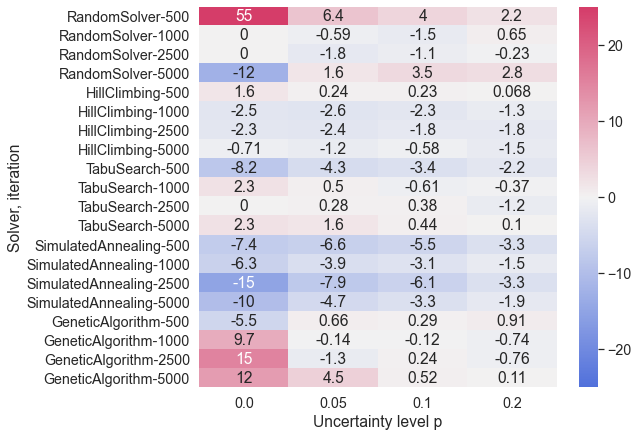
\includegraphics[width=\linewidth]{assets/img/05_Evaluation/heatmap_m1_1.png}
        \caption{Prädiktive gegenüber proaktive Methode}
        \label{fig:evaluation_solver_m1_heatmap_1}
    \end{subfigure}
    \hfill
    \begin{subfigure}{0.497\linewidth}
        \centering
        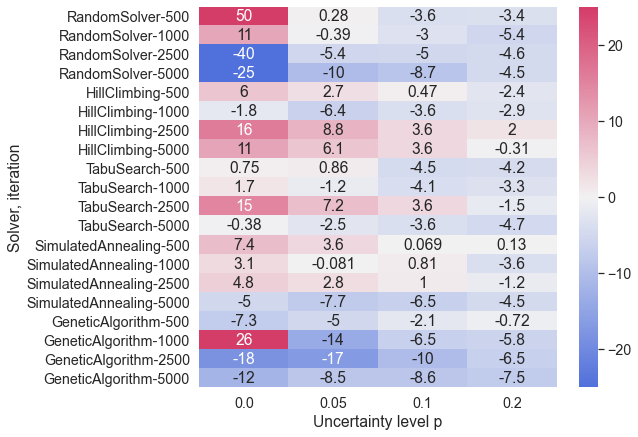
\includegraphics[width=\linewidth]{assets/img/05_Evaluation/heatmap_m1_2.png}
        \caption{Reaktive gegenüber proaktive Methode}
        \label{fig:evaluation_solver_m1_heatmap_2}
    \end{subfigure}
    \par\bigskip 
    \begin{subfigure}{1\linewidth}
        \centering
        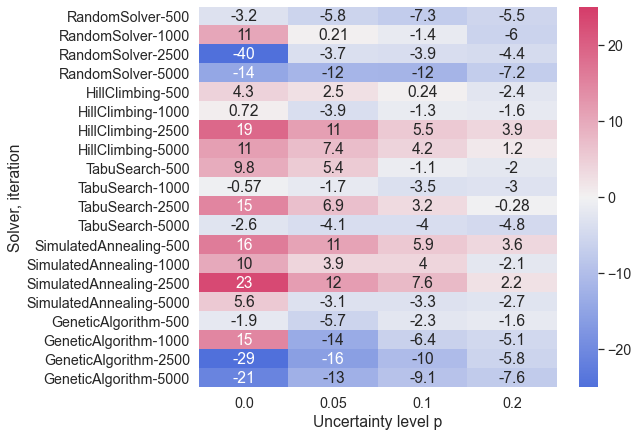
\includegraphics[width=0.5\linewidth]{assets/img/05_Evaluation/heatmap_m1_3.png}
        \caption{Reaktive gegenüber prädiktive Methode}
        \label{fig:evaluation_solver_m1_heatmap_3}
    \end{subfigure}
    
    \caption{Heatmaps der prozentualen Abweichungen für das Instanzset m1}
    \label{fig:evaluation_m1_heatmaps}
    \source{Eigene Darstellungen}
\end{figure}


\begin{figure}[H]

    \begin{subfigure}{0.497\linewidth}
        \centering
        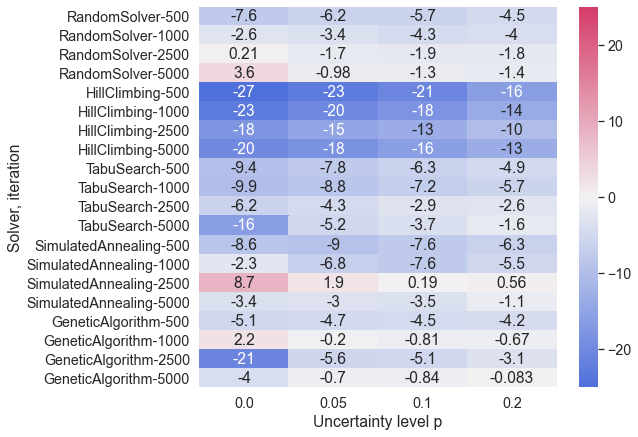
\includegraphics[width=\linewidth]{assets/img/05_Evaluation/heatmap_m2_1.png}
        \caption{Prädiktive gegenüber proaktive Methode}
        \label{fig:evaluation_solver_m2_heatmap_1}
    \end{subfigure}
    \hfill
    \begin{subfigure}{0.497\linewidth}
        \centering
        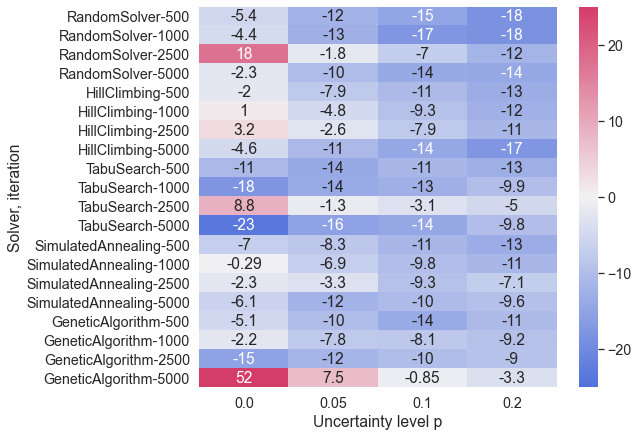
\includegraphics[width=\linewidth]{assets/img/05_Evaluation/heatmap_m2_2.png}
        \caption{Reaktive gegenüber proaktive Methode}
        \label{fig:evaluation_solver_m2_heatmap_2}
    \end{subfigure}
    \par\bigskip 
    \begin{subfigure}{1\linewidth}
        \centering
        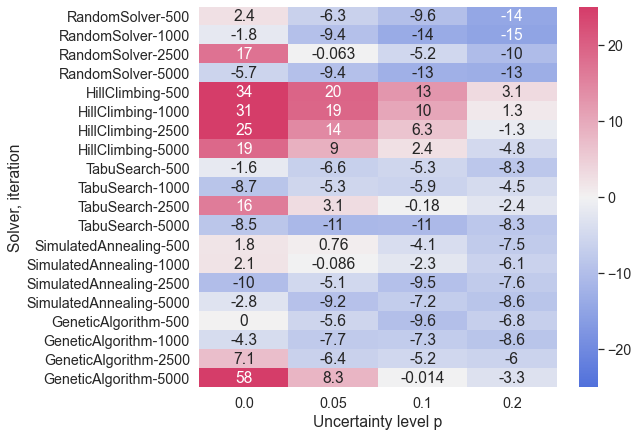
\includegraphics[width=0.5\linewidth]{assets/img/05_Evaluation/heatmap_m2_3.png}
        \caption{Reaktive gegenüber prädiktive Methode}
        \label{fig:evaluation_solver_m2_heatmap_3}
    \end{subfigure}
    
    \caption{Heatmaps der prozentualen Abweichungen für das Instanzset m2}
    \label{fig:evaluation_m2_heatmaps}
    \source{Eigene Darstellungen}
\end{figure}


\begin{figure}[H]

    \begin{subfigure}{0.497\linewidth}
        \centering
        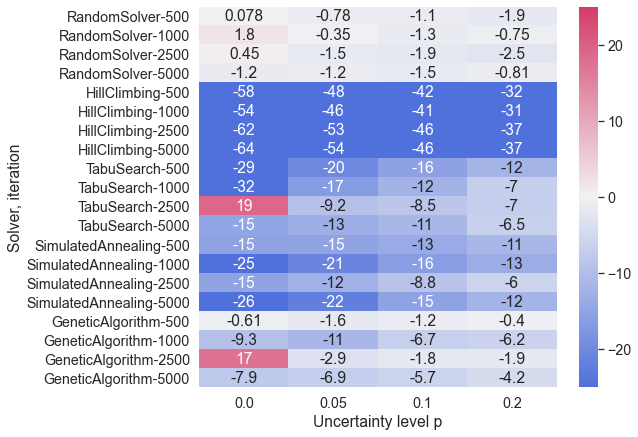
\includegraphics[width=\linewidth]{assets/img/05_Evaluation/heatmap_n0_1.png}
        \caption{Prädiktive gegenüber proaktive Methode}
        \label{fig:evaluation_solver_n0_heatmap_1}
    \end{subfigure}
    \hfill
    \begin{subfigure}{0.497\linewidth}
        \centering
        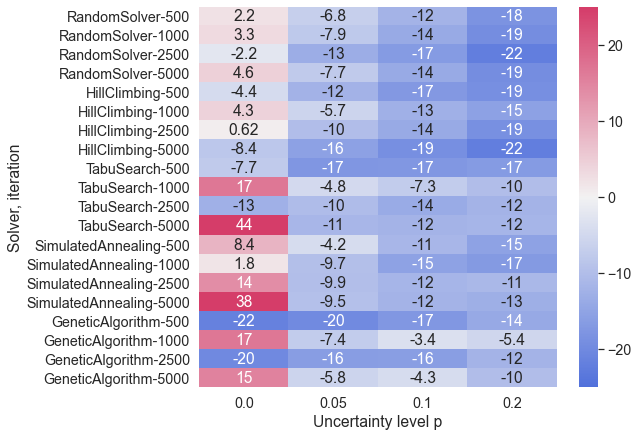
\includegraphics[width=\linewidth]{assets/img/05_Evaluation/heatmap_n0_2.png}
        \caption{Reaktive gegenüber proaktive Methode}
        \label{fig:evaluation_solver_n0_heatmap_2}
    \end{subfigure}
    \par\bigskip 
    \begin{subfigure}{1\linewidth}
        \centering
        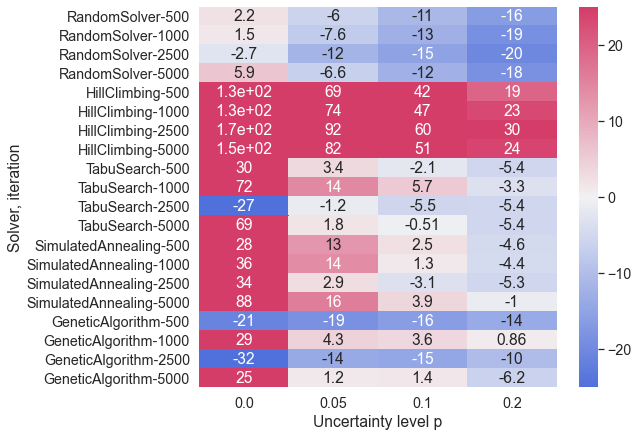
\includegraphics[width=0.5\linewidth]{assets/img/05_Evaluation/heatmap_n0_3.png}
        \caption{Reaktive gegenüber prädiktive Methode}
        \label{fig:evaluation_solver_n0_heatmap_3}
    \end{subfigure}
    
    \caption{Heatmaps der prozentualen Abweichungen für das Instanzset n0}
    \label{fig:evaluation_n0_heatmaps}
    \source{Eigene Darstellungen}
\end{figure}


%-------------
%---Schluss---
%-------------

\backmatter 

\chapter*{Eidesstattliche Erklärung}

Hiermit versichere ich an Eides statt, dass ich diese Arbeit selbstständig verfasst und keine anderen als die angegebenen Quellen und Hilfsmittel benutzt habe. Außerdem versichere ich, dass ich die allgemeinen Prinzipien wissenschaftlicher Arbeit und Veröffentlichung, wie sie in den Leitlinien guter wissenschaftlicher Praxis der Carl von Ossietzky Universität Oldenburg festgelegt sind, befolgt habe.
\vspace{2cm}

\hspace{1cm} \includegraphics[width=0.3\textwidth]{assets/img/UnterschriftOrtDatum.png}  \hfill \includegraphics[width=0.25\textwidth]{assets/img/Unterschrift.png} 
 \hspace{1.3cm}

\hspace{2cm} Ort, Datum \hfill Unterschrift \hspace{2cm} 

\end{document}